% =====================================================================
%  TP Integrador — Filtros analógicos activos
%  Síntesis de Redes Activas — Grupo 3 (LP y BS, Chebyshev I / Elíptica)
% =====================================================================
\documentclass[11pt,a4paper]{article}

% ---------- Idioma y tipografía ----------
\usepackage[utf8]{inputenc}
\usepackage[T1]{fontenc}
\usepackage{lmodern}
% provide=*: usa spanish.ldf si existe (Overleaf/TeX Live completo) o el locale .ini si no.
\usepackage[english,spanish,provide=*]{babel}
\ifdefined\spanishdeactivate\spanishdeactivate{<>.}\fi   % sin atajos < > ni punto decimal especial (equivale a es-nodecimaldot)
\addto\captionsspanish{\renewcommand{\tablename}{Tabla}\renewcommand{\listtablename}{Índice de tablas}}   % equivale a es-tabla
\usepackage{microtype}

% ---------- Página ----------
\usepackage[margin=2.5cm]{geometry}
\usepackage{fancyhdr}
\pagestyle{fancy}
\fancyhf{}
\lhead{\small Filtros analógicos activos — TP integrador}
\rhead{\small Grupo 3}
\cfoot{\thepage}
\setlength{\headheight}{14pt}

% ---------- Matemática, unidades, tablas, figuras ----------
\usepackage{amsmath,amssymb,mathtools}
\usepackage[output-decimal-marker={,},group-separator={.},per-mode=symbol]{siunitx}
\sisetup{group-minimum-digits=5}
\usepackage{booktabs,array,tabularx,multirow}
\usepackage{graphicx}
\usepackage{float}
\usepackage{caption,subcaption}
\captionsetup{font=small,labelfont=bf}
\usepackage[dvipsnames]{xcolor}
\usepackage{enumitem}
\usepackage{fancyvrb}
\setlist{nosep,leftmargin=*}

% ---------- Rutas: funciona compilando desde informe/ o desde la raíz ----------
\graphicspath{{../figuras/}{figuras/}}
\IfFileExists{../resultados/tab_orden.tex}{\newcommand{\resdir}{../resultados}}{\newcommand{\resdir}{resultados}}
\newcommand{\tabres}[1]{\input{\resdir/#1}}
\input{\resdir/valores_nb02}   % valores numéricos generados por el notebook 02
\input{\resdir/valores_nb03}   % valores numéricos generados por el notebook 03
\IfFileExists{\resdir/valores_nb04.tex}{\input{\resdir/valores_nb04}}{}   % mediciones (notebook 04), cuando existan
\IfFileExists{\resdir/valores_nb05.tex}{\input{\resdir/valores_nb05}}{}   % Monte Carlo (notebook 05, Nivel II)
\IfFileExists{\resdir/valores_nb06.tex}{\input{\resdir/valores_nb06}}{}   % ecualizador (notebook 06, Nivel III)
\IfFileExists{../ltspice/filtro_TL072_ac.cir}{\newcommand{\ltsdir}{../ltspice}}{\newcommand{\ltsdir}{ltspice}}

% ---------- Referencias cruzadas y bibliografía ----------
\usepackage[hidelinks]{hyperref}
\usepackage[nameinlink,noabbrev]{cleveref}
\crefname{figure}{figura}{figuras}\Crefname{figure}{Figura}{Figuras}
\crefname{table}{tabla}{tablas}\Crefname{table}{Tabla}{Tablas}
\crefname{equation}{ecuación}{ecuaciones}\Crefname{equation}{Ecuación}{Ecuaciones}
\crefname{section}{sección}{secciones}\Crefname{section}{Sección}{Secciones}
\crefname{subsection}{sección}{secciones}\Crefname{subsection}{Sección}{Secciones}
\crefname{subsubsection}{sección}{secciones}\Crefname{subsubsection}{Sección}{Secciones}
\newcommand{\crefpairconjunction}{ y }\newcommand{\crefmiddleconjunction}{, }\newcommand{\creflastconjunction}{ y }
\newcommand{\crefrangeconjunction}{ a }\newcommand{\crefpairgroupconjunction}{ y }\newcommand{\crefmiddlegroupconjunction}{, }
\newcommand{\creflastgroupconjunction}{ y }
\usepackage[fixlanguage]{babelbib}
\selectbiblanguage{spanish}

% ---------- Macros ----------
\newcommand{\dB}{\,\mathrm{dB}}
\newcommand{\Ap}{A_p}
\newcommand{\As}{A_s}
\newcommand{\jw}{j\omega}
\newcommand{\nr}[2]{\num[round-mode=places,round-precision=#1]{#2}}          % número redondeado
\newcommand{\qr}[3]{\qty[round-mode=places,round-precision=#1]{#2}{#3}}      % magnitud redondeada
\newcommand{\pendiente}[1]{\par\noindent\textcolor{gray}{\emph{[Pendiente: #1]}}\par}

% ---------- Portada (provisoria) ----------
\title{\textbf{Diseño, simulación e implementación de filtros analógicos activos}\\[4pt]
\large Trabajo Práctico Integrador — Síntesis de Redes Activas\\
Grupo 3: pasabajos y rechazabanda, aproximaciones de Chebyshev I y elíptica}
\author{Grupo 3}
\date{\today}

\begin{document}
\maketitle
\thispagestyle{empty}

\begin{abstract}
\noindent
Este informe documenta el diseño, la síntesis, la simulación y la implementación de un filtro analógico activo a partir de
especificaciones de atenuación. Se estudian matemáticamente dos tipos de filtro (pasabajos y rechazabanda) con dos aproximaciones
(Chebyshev~I y elíptica): se obtiene, en cada caso, el orden mínimo, los polos, los ceros, la ganancia y la descomposición en
secciones de primer y segundo orden, y se verifica el cumplimiento de las especificaciones en toda la banda de paso y de rechazo.
La comparación de magnitud, fase, retardo de grupo y respuesta al escalón fundamenta la elección del filtro a implementar:
un pasabajos Chebyshev~I de orden~3 ($f_p = \qty{1}{\kilo\hertz}$, $A_p = \qty{1}{\decibel}$), que cumple con \qty{17.9}{\decibel}
de margen sobre la atenuación exigida a \qty{4}{\kilo\hertz} y se realiza en cascada con una sección de primer orden y una
bicuadrática. Como esa función tiene exactamente \qty{1}{\decibel} de rizado, un Monte Carlo sobre el circuito muestra que solo el
\qty{\vRendSinMargen}{\percent} de los filtros construidos cumpliría la plantilla; por eso se sintetiza una función de diseño Chebyshev~I de orden~3
con \qty{\vApD}{\decibel} de rizado y borde en \qty{\vFpD}{\hertz}, que eleva el rendimiento estimado a más del \qty{98}{\percent}. La realización
usa una red RC con seguidor y un Sallen--Key de ganancia unitaria (TL072CP), cuya transferencia se deriva simbólicamente con SymPy, con los
capacitores disponibles en el laboratorio y resistencias E24 al \qty{1}{\percent}. El prototipo medido cumple la plantilla, con
\IfFileExists{\resdir/valores_nb04.tex}{\qr{2}{\mApMaxMed}{\decibel} de atenuación máxima en la banda de paso y \qr{1}{\mAcuatrokMed}{\decibel} a
\qty{4}{\kilo\hertz}}{}. En el Nivel~II, un Monte Carlo de \nNRun{} corridas por escenario en LTspice, contrastado con Python y con la predicción
por sensibilidades, estima que con los componentes usados cumple la plantilla el \qty{\nRendLtDos}{\percent} de los filtros, y el
\qty{100}{\percent} con capacitores de \qty{\pm 5}{\percent}. En el Nivel~III, un ecualizador pasatodo de 2.º orden con un solo AO, diseñado para
el prototipo y sintonizado a partir de su medición\IfFileExists{\resdir/valores_nb06.tex}{, reduce \num{\eMMejora} veces la variación del retardo
de grupo en la banda de paso (de \qr{3}{\eMJFil}{\milli\second} a \qr{4}{\eMJCas}{\milli\second})}{}. El trabajo es reproducible a partir de los notebooks de Python,
los archivos de LTspice y los datos del repositorio del grupo.
\end{abstract}


\tableofcontents
\clearpage

\section{Introducción y objetivos}
\label{sec:introduccion}

El objetivo del trabajo es recorrer el ciclo completo de diseño de un filtro analógico activo: desde la función de transferencia
ideal que satisface una plantilla de atenuación hasta un prototipo medido en el laboratorio, contrastando en cada paso el modelo
matemático, el modelo circuital y el comportamiento real~\cite{guia2026}. Al grupo~3 le corresponden los tipos \emph{pasabajos}
(LP) y \emph{rechazabanda} (BS), estudiados con las aproximaciones de \emph{Chebyshev~I} y \emph{elíptica} (Cauer).

El alcance se organiza en tres niveles:
\begin{itemize}
  \item \textbf{Nivel~I (obligatorio).} Cuatro diseños matemáticos (2~tipos $\times$ 2~aproximaciones) con su comparación;
        elección, síntesis y análisis simbólico de un único filtro; selección de componentes y del amplificador operacional (AO);
        sensibilidades; validación en LTspice; construcción y medición del prototipo.
  \item \textbf{Nivel~II (optativo).} Análisis estadístico de tolerancias (Monte Carlo) del filtro construido y comparación
        con la predicción lineal basada en sensibilidades.
  \item \textbf{Nivel~III (optativo).} Diseño, simulación, construcción y medición de un ecualizador de fase (pasatodo) que
        reduzca la variación del retardo de grupo del filtro elegido.
\end{itemize}

La metodología de síntesis sigue la de la cátedra~\cite{apuntes2026}, basada en Daryanani~\cite{daryanani1976}:
aproximación, descomposición en cascada de secciones de primer y segundo orden, realización con topologías de un solo AO
mediante igualación de coeficientes y escaleo de impedancia y frecuencia, y evaluación de sensibilidades.

\section{Especificaciones}
\label{sec:especificaciones}

Para ambos tipos se exige una atenuación máxima en la banda de paso $A_p = \qty{1}{\decibel}$ y una atenuación mínima en la banda de
rechazo $A_s = \qty{24}{\decibel}$, con los bordes de la \cref{tab:especificaciones}.

\begin{table}[H]
  \centering
  \caption{Plantilla de atenuación asignada al grupo~3.}
  \label{tab:especificaciones}
  \begin{tabular}{@{}lccc@{}}
    \toprule
    Tipo & Banda(s) de paso & Banda de rechazo & $A_p$ / $A_s$ \\
    \midrule
    Pasabajos (LP)     & $f \le \qty{1000}{\hertz}$ & $f \ge \qty{4000}{\hertz}$ & \qty{1}{\decibel} / \qty{24}{\decibel} \\
    Rechazabanda (BS)  & $f \le \qty{500}{\hertz}$ \;o\; $f \ge \qty{5500}{\hertz}$ & $\qty{1200}{\hertz} \le f \le \qty{2400}{\hertz}$ & \qty{1}{\decibel} / \qty{24}{\decibel} \\
    \bottomrule
  \end{tabular}
\end{table}

\paragraph{Convenciones.} La atenuación se define como
\begin{equation}
  A(\omega) = -20\log_{10}\lvert H(\jw)\rvert \quad [\mathrm{dB}],
  \label{eq:atenuacion}
\end{equation}
referida al máximo de $\lvert H(\jw)\rvert$; es decir, las funciones se normalizan con $\max_\omega \lvert H(\jw)\rvert = 1$ (convención
de \texttt{scipy.signal}~\cite{virtanen2020}). Las frecuencias se especifican en hertz y se convierten a rad/s con $\omega = 2\pi f$ para
todo el cálculo. Una función \emph{cumple} la plantilla si $A(\omega) \le A_p$ en \emph{toda} la banda de paso y $A(\omega) \ge A_s$ en
\emph{toda} la banda de rechazo, no solo en los bordes.

\section{Metodología y herramientas}
\label{sec:metodologia}

\paragraph{Cadena de validación.} Cada etapa se contrasta con la anterior, de modo que toda discrepancia pueda atribuirse a una causa
concreta:
\begin{enumerate}
  \item \textbf{Función objetivo} $H_t(s)$: aproximación obtenida con \texttt{scipy.signal} en forma ceros--polos--ganancia (zpk),
        validada contra las expresiones analíticas de cada aproximación.
  \item \textbf{Función del circuito} $H_c(s)$: análisis nodal simbólico con SymPy~\cite{meurer2017} y AO ideal; se identifica
        $\omega_0$, $Q$ y ganancia de cada sección y se compara con $H_t(s)$.
  \item \textbf{Componentes comerciales}: recálculo de $H_c(s)$ con valores normalizados (series E) y estudio de sensibilidades.
  \item \textbf{LTspice}~\cite{ltspice}: circuito con AO ideal y con el modelo del fabricante; análisis AC y transitorio.
  \item \textbf{Prototipo}: medición de amplitud y fase en las bandas de paso, de transición y de rechazo.
\end{enumerate}

\paragraph{Herramientas.} Python con NumPy~\cite{harris2020}, SciPy~\cite{virtanen2020}, SymPy~\cite{meurer2017},
Matplotlib~\cite{hunter2007} y pandas (notebooks ejecutables en Google Colab), LTspice para la simulación circuital, \LaTeX{} para el
informe y un repositorio Git con las fuentes, los datos y un \texttt{README} con instrucciones de reproducción y versiones de las
bibliotecas. Las figuras y tablas numéricas de este informe se generan directamente desde los notebooks (carpetas
\texttt{figuras/} y \texttt{resultados/}), de modo que tablas, figuras y valores citados en el texto salen de los mismos cálculos y no de transcripciones manuales.

\paragraph{Criterios numéricos.} Se trabaja en forma zpk y en secciones de segundo orden en lugar de coeficientes polinomiales, que
están mal condicionados para órdenes altos. El retardo de grupo se calcula analíticamente a partir de polos y ceros
(\cref{eq:retardo}), con $\omega$ en rad/s, y se contrasta con la derivada numérica de la fase desenrollada.

\section{Diseño matemático}
\label{sec:diseno}

\subsection{Aproximaciones utilizadas}

\subsubsection{Chebyshev~I}
La aproximación de Chebyshev~I distribuye el error en forma equirrizada en la banda de paso y es monótona en la banda de rechazo.
Sobre el prototipo pasabajos normalizado ($\Omega = \omega/\omega_p$):
\begin{equation}
  \lvert H(j\Omega)\rvert^2 = \frac{1}{1+\varepsilon^2 C_N^2(\Omega)}, \qquad
  C_N(\Omega) =
  \begin{cases}
    \cos\!\left(N\arccos\Omega\right), & \lvert\Omega\rvert \le 1,\\
    \cosh\!\left(N\,\mathrm{arccosh}\,\Omega\right), & \lvert\Omega\rvert > 1,
  \end{cases}
  \label{eq:cheby}
\end{equation}
con $\varepsilon^2 = 10^{A_p/10}-1$ ($\varepsilon = \num{0.5088}$ para $A_p = \qty{1}{\decibel}$). Exigir $A(\Omega_s) \ge A_s$ conduce al orden mínimo
\begin{equation}
  N \ge \frac{\mathrm{arccosh}\sqrt{D}}{\mathrm{arccosh}\,\Omega_s}, \qquad D = \frac{10^{A_s/10}-1}{10^{A_p/10}-1},
  \label{eq:orden_cheby}
\end{equation}
con $\sqrt{D} = \num{31.085}$. Los polos se ubican sobre una elipse:
\begin{equation}
  \begin{gathered}
  p_k = \omega_p\left[-\sinh a\,\sin\theta_k + j\cosh a\,\cos\theta_k\right],\qquad k = 1,\dots,N,\\
  a = \frac{1}{N}\,\mathrm{arcsinh}\frac{1}{\varepsilon},\qquad \theta_k = \frac{(2k-1)\pi}{2N}.
  \end{gathered}
  \label{eq:polos_cheby}
\end{equation}
Como $C_N(0) = 0$ para $N$ impar y $\lvert C_N(0)\rvert = 1$ para $N$ par, la ganancia en continua es \qty{0}{\decibel} en el primer caso y $-A_p$ en el segundo.

\subsubsection{Elíptica (Cauer)}
La aproximación elíptica es equirrizada en ambas bandas:
\begin{equation}
  \lvert H(j\Omega)\rvert^2 = \frac{1}{1+\varepsilon^2 R_N^2(\Omega)},
  \label{eq:elip}
\end{equation}
donde $R_N$ es la función racional de Chebyshev (o elíptica), que oscila entre $\pm1$ para $\lvert\Omega\rvert\le1$ y cumple
$\lvert R_N\rvert \ge \sqrt{D}$ para $\lvert\Omega\rvert \ge \Omega_s$. Sus polos sobre el eje imaginario son \emph{ceros de transmisión}
de $H$, lo que produce la transición más abrupta posible para un orden dado. El orden mínimo surge de la ecuación de grado
\begin{equation}
  N \ge \frac{K(k)\,K\!\left(\sqrt{1-k_1^2}\right)}{K\!\left(\sqrt{1-k^2}\right)K(k_1)},\qquad k = \frac{1}{\Omega_s},\qquad k_1 = \frac{1}{\sqrt{D}},
  \label{eq:orden_elip}
\end{equation}
donde $K(\cdot)$ es la integral elíptica completa de primera especie. Para $N$ par, $\lvert H(0)\rvert$ vale $-A_p$ y
$\lvert H(j\infty)\rvert$ vale $-A_s$: la atenuación en alta frecuencia no crece indefinidamente.

\subsubsection{Transformación pasabajos--rechazabanda}
El rechazabanda se obtiene del prototipo pasabajos mediante
\begin{equation}
  s_{LP} = \frac{B\,s}{s^2+\omega_0^2},\qquad \omega_0^2 = \omega_{p1}\,\omega_{p2},\qquad B = \omega_{p2}-\omega_{p1},
  \label{eq:transf_bs}
\end{equation}
que en el eje $\jw$ da $\Omega(\omega) = B\omega/(\omega_0^2-\omega^2)$: los bordes de paso van a $\Omega = 1$ y cada borde de rechazo a
$\Omega(\omega_{s,i})$. El prototipo debe cumplir el peor caso, $\Omega_s = \min_i \lvert\Omega(\omega_{s,i})\rvert$. Cada polo del prototipo
genera un par de polos (el orden se duplica), los ceros en infinito del prototipo se transforman en ceros sobre $\pm j\omega_0$ y cada cero
finito $\pm j\Omega_z$ genera dos pares de ceros con simetría geométrica respecto de $\omega_0$.

\paragraph{Asimetría de la plantilla BS.} La plantilla no es geométricamente simétrica:
$500\times5500 = \qty{2.75e6}{\hertz\squared}$, mientras que $1200\times2400 = \qty{2.88e6}{\hertz\squared}$. Con los bordes de paso
especificados, el borde de rechazo de \qty{2400}{\hertz} resulta el peor caso ($\Omega_s = \num{3.987}$) y Chebyshev~I requiere
$N = \num{2.005} \to 3$, es decir, un rechazabanda de orden~6. Sin embargo, la especificación solo exige banda de paso \emph{hasta}
\qty{500}{\hertz}: ensanchar el borde inferior a
\begin{equation}
  f_{p1}' = \frac{f_{s1} f_{s2}}{f_{p2}} = \frac{1200\times2400}{5500} = \qty{523.6}{\hertz} \;\ge\; \qty{500}{\hertz}
\end{equation}
es más exigente que la plantilla (la contiene) y vuelve simétrico el problema, con $\Omega_s = \num{4.147}$ y $N = \num{1.966} \to 2$
(orden total~4). La alternativa de mover el borde superior ($f_{p2}' = 2{,}88\times10^6/500 = \qty{5760}{\hertz}$) no es válida porque
\emph{estrecharía} la banda de paso. Se ahorra así una sección bicuadrática completa sin violar ninguna especificación; es el mismo criterio
que aplican \texttt{cheb1ord} y \texttt{ellipord} para filtros de banda. La \cref{tab:orden} resume el cálculo analítico, que coincide
con SciPy en los cuatro casos.

\begin{table}[H]
  \centering\small
  \caption{Orden mínimo según las \cref{eq:orden_cheby,eq:orden_elip}. Para el BS, $N$ es el orden del prototipo (orden total $2N$).}
  \label{tab:orden}
  \tabres{tab_orden}
\end{table}

\subsection{Resultados de los cuatro diseños}

Los diseños se obtuvieron con \texttt{cheb1ord}/\texttt{ellipord} (orden y frecuencia de diseño) y \texttt{cheby1}/\texttt{ellip} con
\texttt{analog=True} y \texttt{output='zpk'}. Para Chebyshev~I y la elíptica la frecuencia de diseño es el borde de la banda de rizado:
$f_p = \qty{1000}{\hertz}$ (LP) y $f_{p1}' = \qty{523.64}{\hertz}$, $f_{p2} = \qty{5500}{\hertz}$ (BS). Todos los polos tienen parte real
negativa (diseños estables). Cada par de polos complejos $p,\bar p$ define una sección $s^2 + (\omega_0/Q)s + \omega_0^2$ con
\begin{equation}
  \omega_0 = \lvert p\rvert, \qquad Q = \frac{\lvert p\rvert}{-2\,\mathrm{Re}\,p},
  \label{eq:w0Q}
\end{equation}
y cada polo real $-\sigma$ una sección $s+\sigma$. Los ceros sobre el eje $\jw$ se aparean con el par de polos de $\omega_0$ más cercano.
La \cref{tab:secciones} resume las secciones y la \cref{fig:polos_ceros} muestra los diagramas de polos y ceros.

\begin{table}[H]
  \centering\small
  \caption{Descomposición de los cuatro diseños en secciones de primer y segundo orden.}
  \label{tab:secciones}
  \tabres{tab_secciones}
\end{table}

\begin{figure}[H]
  \centering
  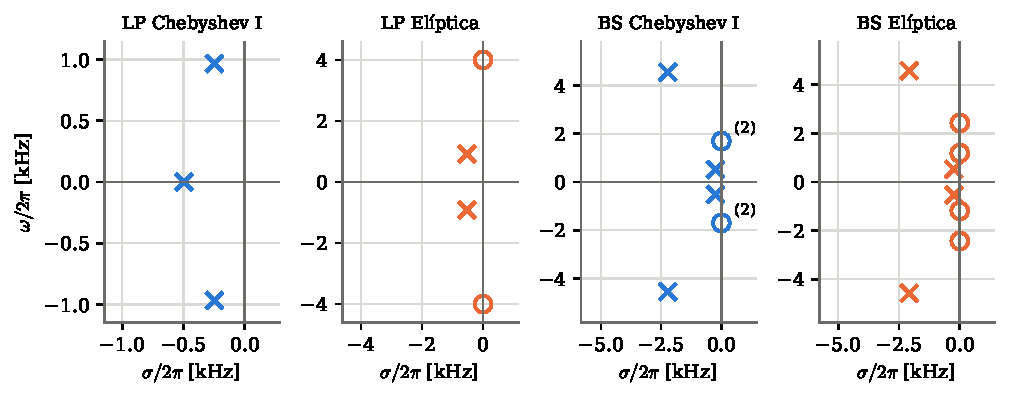
\includegraphics[width=\linewidth]{fig_polos_ceros}
  \caption{Polos ($\times$) y ceros ($\circ$) de los cuatro diseños, en el plano $s/2\pi$ [kHz]. El número entre paréntesis indica
  multiplicidad: el BS Chebyshev~I tiene ceros dobles en $\pm j\,2\pi\cdot\qty{1697.1}{\hertz}$.}
  \label{fig:polos_ceros}
\end{figure}

\paragraph{LP Chebyshev~I (orden~3).}
\begin{equation}
  H(s) = \frac{\num{1.2187e11}}{s^3 + \num{6209.9}\,s^2 + \num{4.8890e7}\,s + \num{1.2187e11}}
       = \underbrace{\frac{\omega_r}{s+\omega_r}}_{T_1(s)}\;
         \underbrace{\frac{\omega_0^2}{s^2 + \frac{\omega_0}{Q}s + \omega_0^2}}_{T_2(s)},
  \label{eq:H_LP_cheb}
\end{equation}
con $\omega_r = \qty{3105.0}{\radian\per\second}$ ($f_r = \qty{494.2}{\hertz}$), $\omega_0 = \qty{6265.0}{\radian\per\second}$
($f_0 = \qty{997.1}{\hertz}$) y $Q = \num{2.018}$; $H(0) = 1$ (\qty{0}{\decibel}). Los polos de la \cref{eq:polos_cheby} coinciden con los
de SciPy con error relativo $\num{4e-16}$. Para $N = 3$ se verifica además que $\omega_0/Q = \omega_r$, pues $\sin\theta_2 = 1$ y
$\sin\theta_1 = 1/2$ en la \cref{eq:polos_cheby}.

\paragraph{LP elíptico (orden~2).}
\begin{equation}
  H(s) = \num{0.063096}\,\frac{s^2 + \omega_z^2}{s^2 + \frac{\omega_0}{Q}s + \omega_0^2},
  \label{eq:H_LP_elip}
\end{equation}
con $\omega_z = \qty{25166}{\radian\per\second}$ ($f_z = \qty{4005.3}{\hertz}$), $\omega_0 = \qty{6696.0}{\radian\per\second}$
($f_0 = \qty{1065.7}{\hertz}$) y $Q = \num{1.009}$. Resulta $H(0) = \num{0.8913}$ (\qty{-1}{\decibel}) y $H(j\infty) = \num{0.0631}$
(\qty{-24}{\decibel}).

\paragraph{BS Chebyshev~I (orden~4).}
\begin{equation}
  H(s) = H_0 \prod_{i=1}^{2} \frac{\omega_{0i}^2}{\omega_z^2}\,\frac{s^2+\omega_z^2}{s^2 + \frac{\omega_{0i}}{Q_i}s + \omega_{0i}^2},
  \qquad H_0 = \num{0.8913},
  \label{eq:H_BS}
\end{equation}
con ceros dobles en $\omega_z = \qty{10663}{\radian\per\second}$ ($f_z = \qty{1697.1}{\hertz} = \sqrt{1200\times2400}$\,Hz) y secciones
$f_{01} = \qty{568.4}{\hertz}$, $f_{02} = \qty{5066.8}{\hertz}$, ambas con $Q = \num{1.137}$. Los dos pares de polos son geométricamente
simétricos: $\omega_{01}\omega_{02} = \omega_z^2$.

\paragraph{BS elíptico (orden~4).} Misma forma que la \cref{eq:H_BS}, pero cada sección tiene su propio cero:
$f_{z1} = \qty{1186.0}{\hertz}$ (sección $f_{01} = \qty{572.9}{\hertz}$, $Q = \num{1.210}$) y $f_{z2} = \qty{2428.4}{\hertz}$ (sección
$f_{02} = \qty{5026.9}{\hertz}$, $Q = \num{1.210}$). La primera es una sección \emph{notch} pasabajos ($f_z > f_0$) y la segunda una
\emph{notch} pasaaltos ($f_z < f_0$); $f_{z1}f_{z2} = f_{01}f_{02} = \qty{2.88e6}{\hertz\squared}$.

\subsection{Verificación de especificaciones}

La atenuación se evaluó en una grilla logarítmica densa (\num{3000} puntos por banda, incluidos los bordes exactos) sobre toda la banda de
paso (desde \qty{1}{\hertz}) y toda la banda de rechazo (hasta \qty{1}{\mega\hertz}). La \cref{tab:verificacion} muestra que los cuatro
diseños cumplen y que ninguno cumple con un orden de prototipo menor, lo que confirma que el orden es mínimo.

\begin{table}[H]
  \centering
  \caption{Verificación de la plantilla. Margen: $A_{s,\min} - A_s$.}
  \label{tab:verificacion}
  \footnotesize
  \tabres{tab_verificacion}
\end{table}

Dos observaciones. Primero, el LP Chebyshev~I de orden~3 cumple con \qty{17.9}{\decibel} de margen a \qty{4}{\kilo\hertz}, porque el orden~2
falla por muy poco ($N = \num{2.001}$ en la \cref{tab:orden}) y el salto a orden~3 sobredimensiona la selectividad. Segundo, los diseños
elípticos tienen margen nulo en la banda de rechazo por construcción: SciPy fija el rizado de rechazo exactamente en $A_s$ y aprovecha
el orden sobrante para adelantar la transición (el LP elíptico alcanza \qty{24}{\decibel} a \qty{2877}{\hertz}, no a \qty{4000}{\hertz}).
La frecuencia de \qty{-3}{\decibel} es \qty{1094.9}{\hertz} para el Chebyshev~I y \qty{1199.7}{\hertz} para el elíptico.

\subsection{Comparación}

\subsubsection{Magnitud}

\begin{figure}[H]
  \centering
  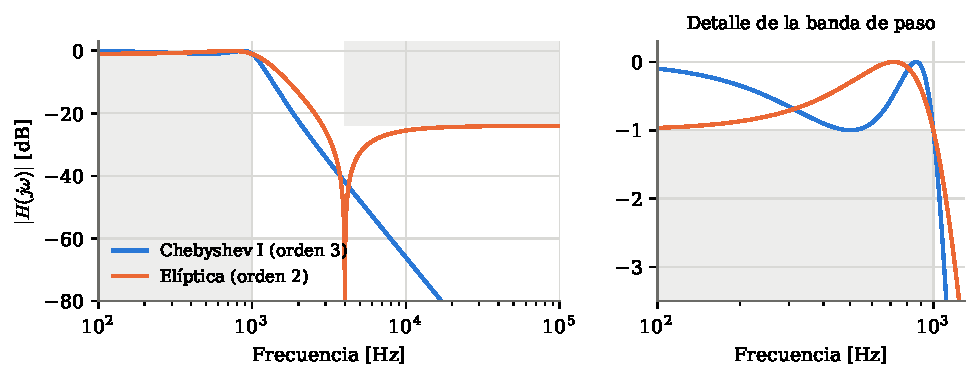
\includegraphics[width=\linewidth]{fig_LP_magnitud}
  \caption{Pasabajos: magnitud de ambas aproximaciones. Las zonas grises son las regiones prohibidas de la plantilla.}
  \label{fig:LP_mag}
\end{figure}

\begin{figure}[H]
  \centering
  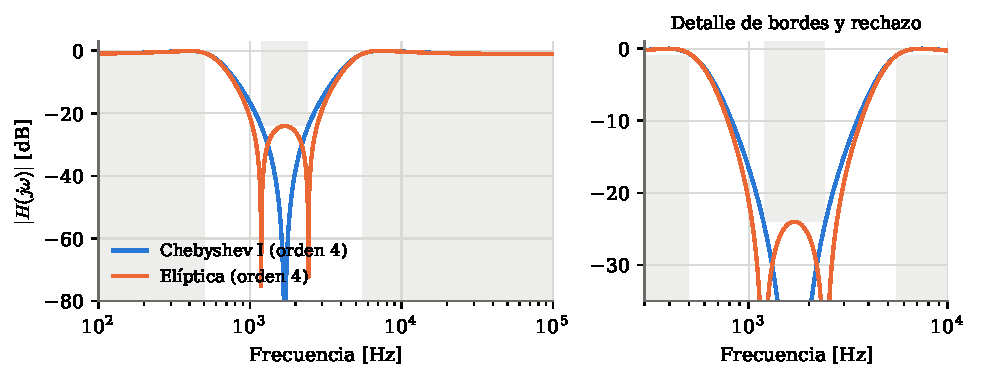
\includegraphics[width=\linewidth]{fig_BS_magnitud}
  \caption{Rechazabanda: magnitud de ambas aproximaciones y detalle de la transición.}
  \label{fig:BS_mag}
\end{figure}

En el LP (\cref{fig:LP_mag}) el elíptico resuelve la plantilla con orden~2 gracias al cero de transmisión en \qty{4005}{\hertz}, pero
su atenuación se estabiliza en \qty{24}{\decibel} por encima de esa frecuencia. El Chebyshev~I, en cambio, cae a
\qty{-60}{\decibel}/década sin límite: a \qty{10}{\kilo\hertz} atenúa \qty{66.1}{\decibel} frente a \qty{25.5}{\decibel} del
elíptico, una diferencia relevante para rechazar ruido y armónicos de alta frecuencia. En el BS (\cref{fig:BS_mag}), con el mismo orden,
el elíptico alcanza \qty{47.2}{\decibel} en los bordes de rechazo y empieza a atenuar \qty{24}{\decibel} desde \qty{1040}{\hertz}, frente a
\qty{1186}{\hertz} del Chebyshev~I, cuyo margen en los bordes es de solo \qty{0.62}{\decibel}.

\subsubsection{Fase y retardo de grupo}
El retardo de grupo se calcula analíticamente a partir de los polos $p_i = \sigma_{p_i}+j\omega_{p_i}$ y de los ceros
$z_j = \sigma_{z_j}+j\omega_{z_j}$ que no están sobre el eje $\jw$:
\begin{equation}
  \tau_g(\omega) = -\frac{d\varphi}{d\omega}
  = \sum_i \frac{-\sigma_{p_i}}{\sigma_{p_i}^2+(\omega-\omega_{p_i})^2}
  - \sum_j \frac{-\sigma_{z_j}}{\sigma_{z_j}^2+(\omega-\omega_{z_j})^2},
  \label{eq:retardo}
\end{equation}
y coincide con la derivada numérica de la fase desenrollada con error relativo menor que \num{4e-6}. Los ceros sobre $\jw$ solo
introducen saltos de fase de $\pm\ang{180}$ en $\omega_z$ (cambio de signo de $H$), visibles en las \cref{fig:fase,fig:fase_bs} para los elípticos.
En el BS Chebyshev~I el cero es doble, el salto es de \ang{360} y el desenrollado lo elimina.

\begin{figure}[H]
  \centering
  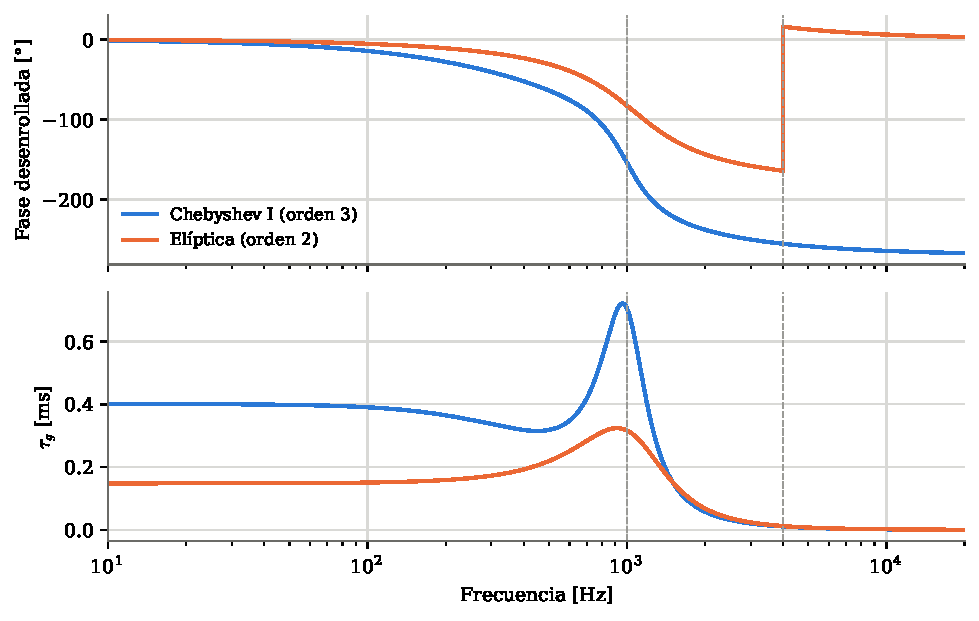
\includegraphics[width=0.92\linewidth]{fig_LP_fase_retardo}
  \caption{Pasabajos: fase desenrollada y retardo de grupo. Las líneas punteadas son los bordes de la plantilla.}
  \label{fig:fase}
\end{figure}

\begin{figure}[H]
  \centering
  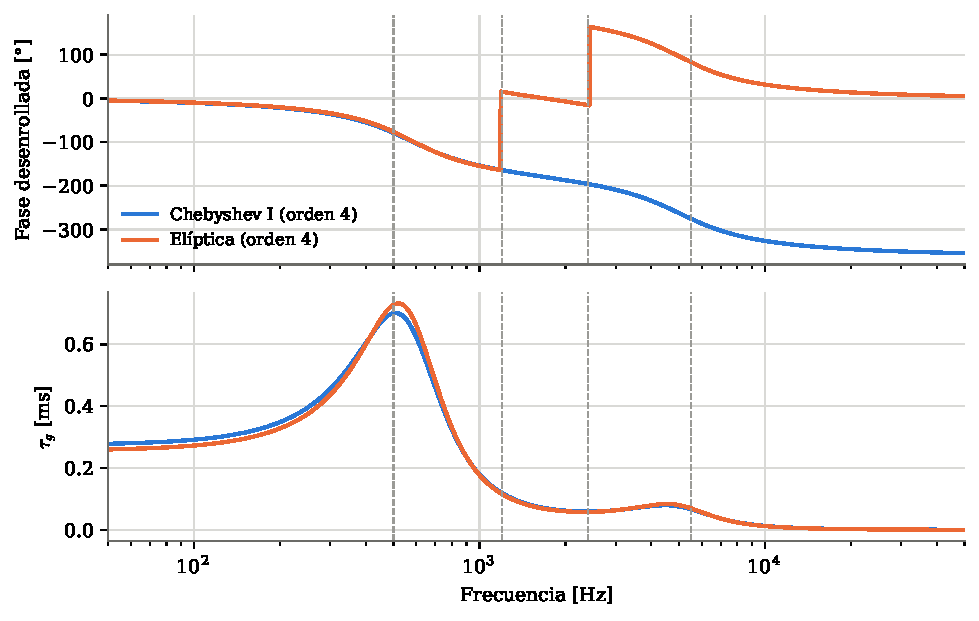
\includegraphics[width=0.92\linewidth]{fig_BS_fase_retardo}
  \caption{Rechazabanda: fase desenrollada y retardo de grupo. Los saltos de la fase del elíptico ocurren en sus ceros de transmisión.}
  \label{fig:fase_bs}
\end{figure}

\subsubsection{Respuesta temporal}

\begin{figure}[H]
  \centering
  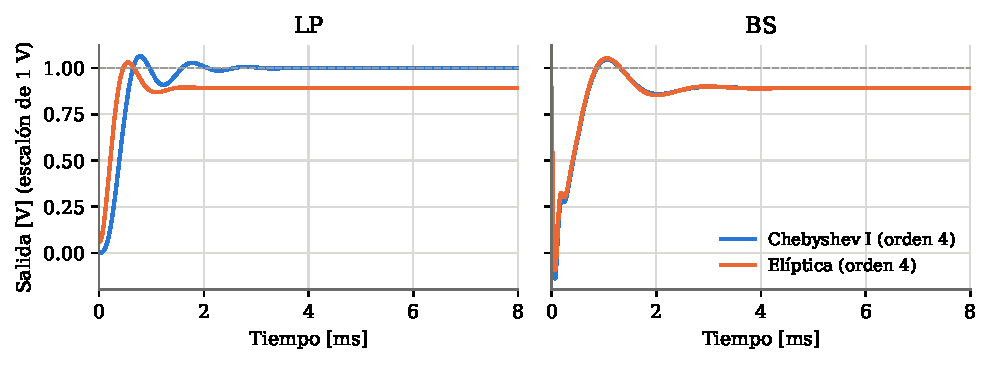
\includegraphics[width=\linewidth]{fig_escalon}
  \caption{Respuesta al escalón unitario.}
  \label{fig:escalon}
\end{figure}

\begin{table}[H]
  \centering\small
  \caption{Comparación de magnitud y de comportamiento temporal. $\Delta\tau_g$: variación del retardo de grupo en la banda de paso.}
  \label{tab:comparativa}
  \tabres{tab_comparativa_magnitud}\\[8pt]
  \tabres{tab_comparativa_tiempo}
\end{table}

La \cref{tab:comparativa} y la \cref{fig:escalon} muestran el compromiso típico entre selectividad y comportamiento temporal. El
Chebyshev~I de orden~3 tiene mayor retardo (\qty{0.40}{\milli\second} en continua) y un pico de \qty{0.72}{\milli\second} cerca del borde
de paso, con una variación de \qty{0.41}{\milli\second} dentro de la banda; su sobrepico es moderado (\qty{6.4}{\percent}) y se establece
al \qty{2}{\percent} en \qty{1.9}{\milli\second}. El elíptico de orden~2 tiene menos retardo pero más sobrepico (\qty{15.5}{\percent}) y,
como el grado de su numerador iguala al del denominador, su salida salta instantáneamente a $H(j\infty) = \num{0.063}$ ante el escalón.
En el BS ambas aproximaciones tienen retardo y respuesta al escalón casi idénticos, porque sus polos son muy parecidos (\cref{tab:secciones}).

\subsection{Elección del filtro y propuesta de implementación}
\label{sec:eleccion}

Se propone implementar el \textbf{pasabajos Chebyshev~I de orden~3} (propuesta de la cátedra, sujeta a aprobación docente). Los motivos
son los siguientes:
\begin{enumerate}
  \item \textbf{Margen de especificación.} Cumple con \qty{17.9}{\decibel} de margen en la banda de rechazo y sigue atenuando a
        \qty{-60}{\decibel}/década, lo que absorbe la dispersión de los componentes (relevante para el análisis de tolerancias del Nivel~II).
        Los elípticos tienen margen nulo por construcción.
  \item \textbf{Función todo polos.} Se realiza con una sección de primer orden y una bicuadrática pasabajos de un solo AO
        (Sallen--Key~\cite{daryanani1976}). Los demás casos requieren bicuadráticas con ceros sobre $\jw$ (secciones notch), con más AO y
        con alta sensibilidad de la frecuencia del cero.
  \item \textbf{Orden impar.} $H(0) = \qty{0}{\decibel}$, sin la pérdida de \qty{1}{\decibel} en continua de los diseños de orden par.
  \item \textbf{$Q$ moderado.} $Q = \num{2.018}$ es realizable con AO de propósito general; la verificación de GBW y slew rate se hace en
        la etapa de selección del AO.
\end{enumerate}
Su contracara es el mayor retardo de grupo y su variación cerca del borde de paso, que es precisamente lo que motiva el ecualizador de
fase del Nivel~III.

\paragraph{Orden de la cascada.} La bicuadrática aislada presenta un pico de $Q/\sqrt{1-1/(4Q^2)} \to \qty{6.37}{\decibel}$ en
\qty{934}{\hertz} (\cref{fig:secciones}). Si se ubicara primero, la señal en el nodo intermedio superaría en \qty{6.4}{\decibel} a la de la
salida y limitaría la amplitud máxima de entrada antes de saturar. Ubicando primero la sección de primer orden, el nodo intermedio nunca
supera la ganancia unitaria, de modo que la salida final es el punto de mayor nivel.

\begin{figure}[H]
  \centering
  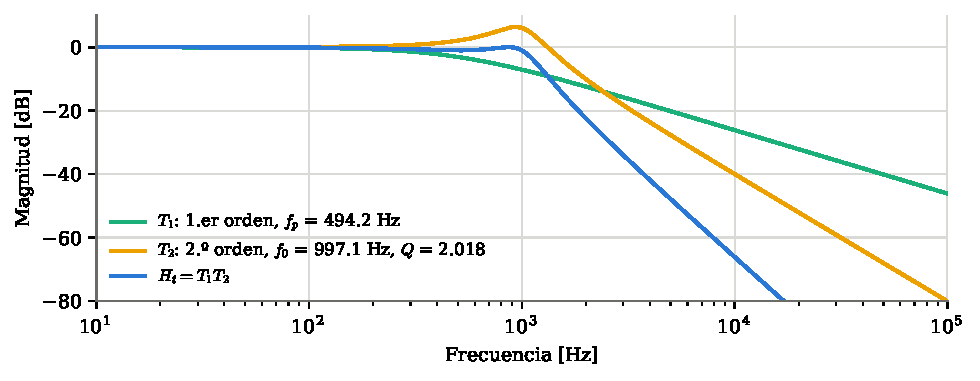
\includegraphics[width=0.85\linewidth]{fig_LP_cheby1_secciones}
  \caption{Descomposición del LP Chebyshev~I en $T_1(s)$ (primer orden) y $T_2(s)$ (bicuadrática). El producto reproduce $H_t(s)$ con
  error menor que \num{1e-15}.}
  \label{fig:secciones}
\end{figure}

\paragraph{Propuesta de implementación.} Etapa~1: polo real con una red RC seguida de un seguidor de tensión, que aísla la red y entrega
a la etapa siguiente la baja impedancia de fuente que exige el Sallen--Key. Etapa~2: Sallen--Key pasabajos para el par complejo. Ambos AO en un
TL072. La síntesis (\cref{sec:sintesis}) incorpora además un \emph{margen de diseño}: como $H_t$ tiene exactamente \qty{1}{\decibel} de rizado,
se sintetiza una función Chebyshev~I de orden~3 algo más exigente, para que las tolerancias de los componentes no lleven el filtro construido fuera
de la plantilla.

% --- Secciones de las semanas 2 a 5 (se habilitan a medida que se completan) ---
\section{Síntesis circuital}
\label{sec:sintesis}

\subsection{Función de diseño con margen}
\label{sec:margen}
La función de la plantilla $H_t(s)$ (\cref{eq:H_LP_cheb}) tiene exactamente $A_p = \qty{1}{\decibel}$ de rizado: el diseño nominal no deja margen
en la banda de paso. El circuito construido no realiza $H_t$, sino una función con $f_r$, $f_0$ y $Q$ desplazados por las tolerancias de los
componentes. Para cuantificarlo se hizo un Monte Carlo analítico sobre el circuito elegido (\cref{sec:topologia}), con distribuciones uniformes e
independientes ($R$: $\pm\qty{1}{\percent}$; $C$: $\pm\qty{5}{\percent}$ o $\pm\qty{10}{\percent}$) y \num{20000} muestras por caso, contando qué
porcentaje de los circuitos cumple la plantilla (\emph{rendimiento}).

Se compararon funciones de diseño Chebyshev~I de orden~3 con rizado $A_{p,d} \le A_p$ y borde $f_{p,d} \ge f_p$. Ambas condiciones son más
exigentes que la plantilla, de modo que el diseño nominal sigue cumpliéndola y la diferencia queda como presupuesto para las tolerancias. El precio es
una menor atenuación a \qty{4}{\kilo\hertz}, donde $H_t$ tiene casi \qty{18}{\decibel} de margen (\cref{tab:margen}).

\begin{table}[H]
  \centering\small
  \caption{Rendimiento estimado según la función de diseño (Chebyshev~I, orden~3). En negrita, la opción adoptada.}
  \label{tab:margen}
  \resizebox{\linewidth}{!}{\tabres{tab_margen}}
\end{table}

Sin margen, solo cumple alrededor del \qty{4}{\percent} de los circuitos. Se adopta la \textbf{función de diseño $H_d$: Chebyshev~I de orden~3 con
$A_{p,d} = \qty{\vApD}{\decibel}$ y $f_{p,d} = \qty{\vFpD}{\hertz}$}. Sigue siendo el filtro aprobado y eleva el rendimiento estimado al
\qty{100}{\percent} con capacitores de $\pm\qty{5}{\percent}$ y a más del \qty{98}{\percent} con $\pm\qty{10}{\percent}$, conservando
\qty{\vAcuatroD}{\decibel} de atenuación nominal a \qty{4}{\kilo\hertz} (\qty{10.7}{\decibel} de margen). Sus parámetros son
$f_r = \qty{\vFrD}{\hertz}$, $f_0 = \qty{\vFoD}{\hertz}$ y $Q = \num{\vQD}$ (\cref{fig:Ht_vs_Hd}). Toda la síntesis que sigue usa $H_d$, pero la
verificación se hace siempre contra la plantilla original.

\begin{figure}[H]
  \centering
  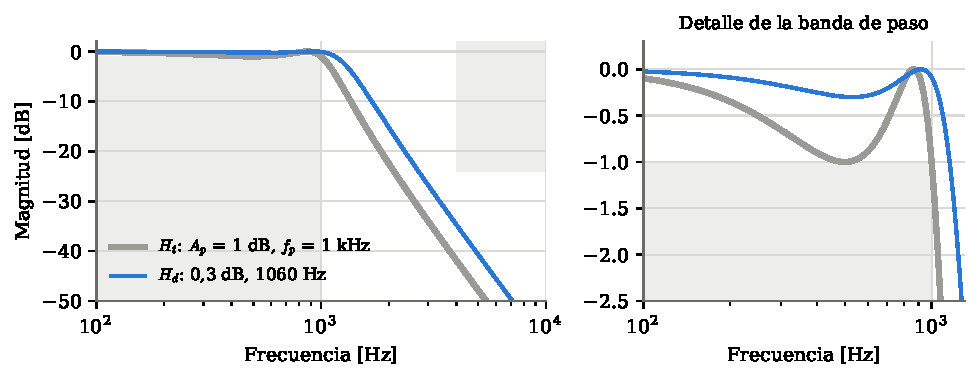
\includegraphics[width=\linewidth]{fig_Ht_vs_Hd}
  \caption{Función de la plantilla $H_t$ y función de diseño con margen $H_d$. La zona gris es la región prohibida de la plantilla.}
  \label{fig:Ht_vs_Hd}
\end{figure}

\subsection{Topología}
\label{sec:topologia}
La función de diseño se realiza en cascada (\cref{fig:esquema}), siguiendo el orden justificado en la \cref{sec:eleccion}:
\begin{itemize}
  \item \textbf{Etapa~1 (polo real):} red $R_0C_0$ seguida de un seguidor de tensión (U1). La resistencia interna del generador $R_s$
        queda en serie con $R_0$ y se incluye en el modelo.
  \item \textbf{Etapa~2 (par complejo):} Sallen--Key pasabajos~\cite[cap.~8]{daryanani1976} de ganancia unitaria ($k = 1$), con U2
        como seguidor.
\end{itemize}
Los nodos se numeran del 0 (masa) al 6 (salida); la misma numeración se usa en el netlist de LTspice.

\begin{figure}[H]
  \centering
  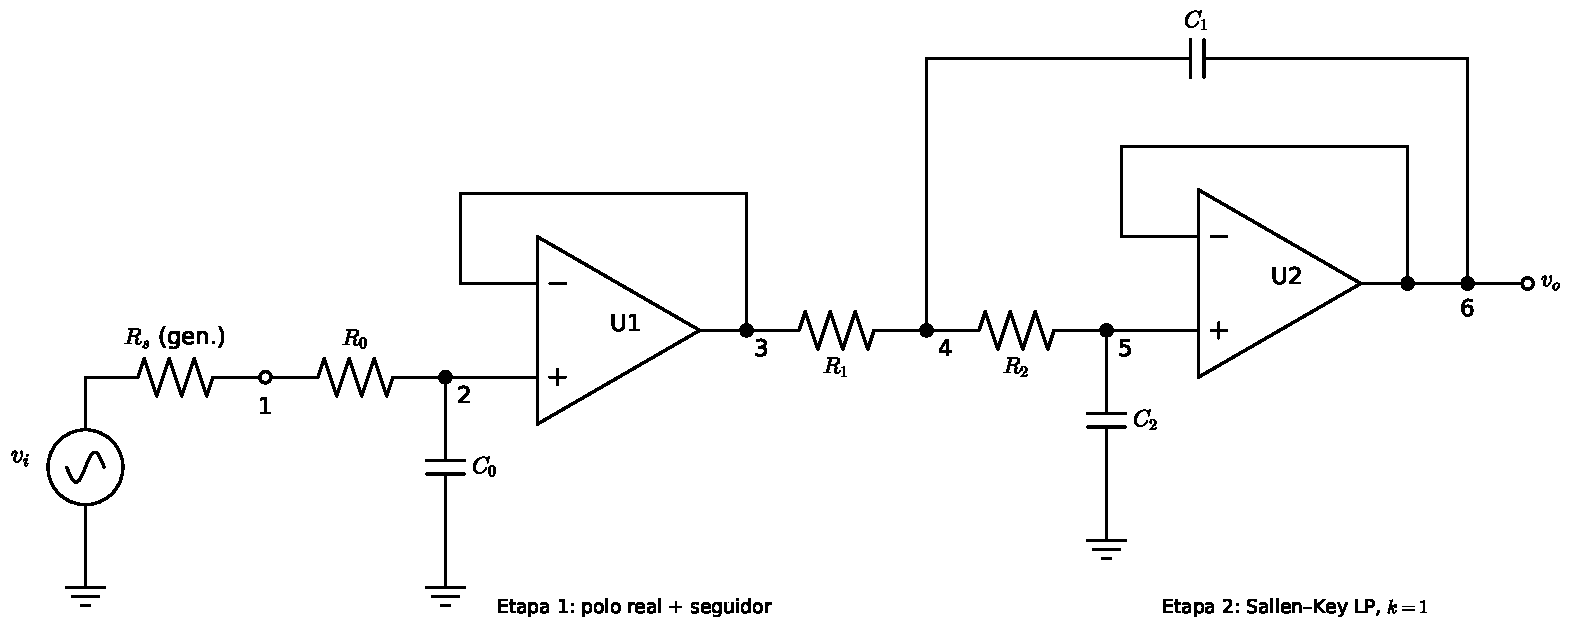
\includegraphics[width=\linewidth]{fig_esquema}
  \caption{Circuito implementado con los nodos numerados. U1 y U2 son las dos mitades de un TL072CP.}
  \label{fig:esquema}
\end{figure}

\subsection{Análisis nodal simbólico}
Con AO ideales (realimentación negativa, $v^+ = v^-$ y corrientes de entrada nulas), las ecuaciones de Kirchhoff en los nodos son
\begin{equation}
\begin{aligned}
  &\text{nodo 1:}\quad \frac{V_i-V_1}{R_s} = \frac{V_1-V_2}{R_0}, &\qquad
  &\text{nodo 2:}\quad \frac{V_1-V_2}{R_0} = sC_0V_2, &\qquad
  &\text{U1:}\quad V_3 = V_2,\\
  &\text{nodo 4:}\quad \frac{V_3-V_4}{R_1} + (V_6-V_4)\,sC_1 + \frac{V_5-V_4}{R_2} = 0, &
  &\text{nodo 5:}\quad \frac{V_4-V_5}{R_2} = sC_2V_5, &
  &\text{U2:}\quad V_6 = V_5.
\end{aligned}
\label{eq:nodales}
\end{equation}
Resolviendo el sistema con SymPy se obtiene
\begin{equation}
  H_c(s) = \frac{V_6}{V_i} =
  \underbrace{\frac{1}{sC_0(R_0+R_s)+1}}_{T_1(s)}\;
  \underbrace{\frac{1}{C_1C_2R_1R_2\,s^2 + C_2(R_1+R_2)\,s + 1}}_{T_2(s)},
  \label{eq:Hc}
\end{equation}
y, por igualación de coeficientes con las formas canónicas,
\begin{equation}
  \omega_r = \frac{1}{C_0(R_0+R_s)},\qquad
  \omega_0 = \frac{1}{\sqrt{R_1R_2C_1C_2}},\qquad
  Q = \sqrt{\frac{C_1}{C_2}}\;\frac{\sqrt{R_1R_2}}{R_1+R_2},\qquad H_c(0) = 1.
  \label{eq:param_circuito}
\end{equation}
Como $\sqrt{R_1R_2} \le (R_1+R_2)/2$, resulta $Q \le \tfrac12\sqrt{C_1/C_2}$: el Sallen--Key de ganancia unitaria exige una relación de
capacitores $n = C_1/C_2 \ge 4Q^2$, que para $H_d$ vale \num{\vCuatroQcuad}. SymPy también confirma que el caso general de ganancia
$k = 1 + r_2/r_1$ reproduce las expresiones (8.6)--(8.8) de Daryanani~\cite{daryanani1976} y que se reduce a la \cref{eq:param_circuito} con
$k = 1$. Con los valores ideales de la síntesis, $\max\lvert H_c - H_d\rvert = \num{\vErrSintesis}$: el circuito reproduce exactamente la función
de diseño.

\subsection{Aislamiento entre etapas}
Si se elimina U1, la red $R_0C_0$ queda cargada por la entrada del Sallen--Key. La diferencia entre los denominadores mónicos de ambos casos es
\begin{equation}
  D_{\text{sin U1}}(s) - D_{\text{con U1}}(s) = \frac{s\,(sC_1R_2+1)}{C_0C_1R_1R_2},
\end{equation}
que solo se anula si $R_1\to\infty$ o $C_0\to\infty$, es decir, si la segunda etapa no carga a la primera. Con los componentes elegidos, omitir el
seguidor produce un error de hasta \qty{\vErrSinBuffer}{\decibel} en la zona de \qty{1}{\kilo\hertz} (la atenuación a \qty{1}{\kilo\hertz} pasa a
ser \qty{\vAmilSinBuffer}{\decibel}, ver \cref{fig:Hc_vs_Ht}), y el filtro deja de cumplir la plantilla. Con U1, el acoplamiento queda acotado por
la impedancia de salida en lazo cerrado del AO, del orden de los miliohms a estas frecuencias, que es despreciable frente a $R_1$.

\subsection{Elección del diseño Sallen--Key}
Antes de imponer igualdades entre componentes se calcularon con SymPy las sensibilidades normalizadas
$S_x^{Q} = \frac{x}{Q}\frac{\partial Q}{\partial x}$ del Sallen--Key general respecto de sus seis elementos, y se evaluaron en los tres diseños de la
cátedra para el $Q$ de $H_d$. La \cref{tab:disenos_sk} incluye además el corrimiento de $Q$ por GBW finito, con $A(s) = \omega_t/s$.

\begin{table}[H]
  \centering
  \caption{Comparación de los diseños Sallen--Key de la cátedra~\cite[tabla~8.1]{daryanani1976} para $Q = \num{\vQD}$.}
  \label{tab:disenos_sk}
  \resizebox{\linewidth}{!}{\tabres{tab_disenos_sk}}
\end{table}

Se adopta el \textbf{diseño~1 (ganancia unitaria) en su forma generalizada}, por estos motivos:
\begin{itemize}
  \item Tiene las menores sensibilidades pasivas. Con $k = 1$ y sin imponer $R_1 = R_2$,
        \begin{equation}
          S^Q_{R_1} = -S^Q_{R_2} = \frac{R_2-R_1}{2(R_1+R_2)},\qquad S^Q_{C_1} = -S^Q_{C_2} = \frac12,\qquad
          S^{\omega_0}_{R_1,R_2,C_1,C_2} = -\frac12 ,
          \label{eq:sens_k1}
        \end{equation}
        de modo que $\lvert S^Q_{R}\rvert < \tfrac12$ para cualquier par de resistencias.
  \item No necesita la red de ganancia $r_1$, $r_2$: tiene menos componentes, $H(0) = 1$ sin ajuste de ganancia y el AO trabaja con máxima
        realimentación.
  \item El GBW finito no decide la elección: el corrimiento de $Q$ es menor que \qty{0.5}{\percent} en los tres diseños, incluso con el LM358.
\end{itemize}
La única desventaja del diseño~1 clásico ($R_1 = R_2$) es que exige $C_1/C_2 = 4Q^2$ exactamente. En la forma generalizada se eligen dos
capacitores disponibles con $n = C_1/C_2 \ge 4Q^2$ y se despejan $R_1$ y $R_2$ de la \cref{eq:param_circuito}. Ambas resistencias son las raíces
de $x^2 - x/(Q\omega_0C_2) + 1/(\omega_0^2C_1C_2) = 0$:
\begin{equation}
  R_{1,2} = \frac{1\pm\sqrt{1-4Q^2/n}}{2\,Q\,\omega_0\,C_2}.
  \label{eq:R12}
\end{equation}

\subsection{Elección de capacitores}
En el laboratorio hay capacitores de \qty{1}{\nano\farad}, \qty{4.7}{\nano\farad}, \qty{10}{\nano\farad}, \qty{47}{\nano\farad},
\qty{100}{\nano\farad} y de \qty{150}{\nano\farad} a \qty{1}{\micro\farad}, además de valores de pF (demasiado chicos para estos niveles de
impedancia) y de \qty{2.2}{\micro\farad} o más (presumiblemente electrolíticos, inadecuados para un filtro). La \cref{tab:capacitores} recorre
todos los pares disponibles con $n \ge 4Q^2$ y resistencias entre \qty{1}{\kilo\ohm} y \qty{200}{\kilo\ohm}.

\begin{table}[H]
  \centering\small
  \caption{Pares de capacitores disponibles para el Sallen--Key, ordenados por sensibilidad de $Q$ a las resistencias. La última columna es el error
  de $f_0$ si cada resistencia se redondea a un único valor E24.}
  \label{tab:capacitores}
  \tabres{tab_capacitores}
\end{table}

Se eligen $C_1 = \qty{47}{\nano\farad}$ y $C_2 = \qty{4.7}{\nano\farad}$ ($n = 10$). Es el par de menor sensibilidad,
$S^Q_{R_1} = \num{\vSQRuno}$: como $n$ queda apenas por encima de $4Q^2$, resulta $R_1 \approx R_2$, cerca del máximo de $Q$ respecto del cociente
$R_1/R_2$. Además da niveles de impedancia de unos \qty{10}{\kilo\ohm}. Para la etapa~1 se toma $C_0 = \qty{10}{\nano\farad}$, de modo que cada
valor de capacitor se usa una sola vez.

\subsection{Diseño normalizado, escaleo y resistencias}
Siguiendo el procedimiento de la cátedra~\cite{apuntes2026}, se diseña primero con $\omega_0 = \qty{1}{\radian\per\second}$ y
$C_2 = \qty{1}{\farad}$. Para $n = 10$, la \cref{eq:R12} da $R = \qty{\vRnMay}{\ohm}$ y $\qty{\vRnMen}{\ohm}$, con $C_1 = \qty{10}{\farad}$. El
escaleo de frecuencia ($k_f = \omega_0 = \qty{\vKf}{\radian\per\second}$) y de impedancia ($k_z = 1/(k_f\cdot\qty{4.7}{\nano\farad}) = \num{\vKz}$)
lleva a $C_2 = \qty{4.7}{\nano\farad}$, $C_1 = \qty{47}{\nano\farad}$, $R_1 = \qty{\vRunoId}{\kilo\ohm}$ y $R_2 = \qty{\vRdosId}{\kilo\ohm}$. El escaleo
no modifica $Q$. Para la etapa~1, $R_0 + R_s = 1/(\omega_r C_0) = \qty{\vRceroMasRs}{\kilo\ohm}$, es decir, $R_0 = \qty{\vRceroId}{\kilo\ohm}$.

Las resistencias son del \qty{1}{\percent} en valores E24. Redondear cada una a un único valor corre $f_0$ casi \qty{2}{\percent}, de modo que cada
resistencia se arma con dos valores E24 en serie (\cref{tab:resistencias}). El error residual queda en el orden de \qty{0.1}{\percent}, diez
veces menor que la tolerancia de cada resistencia.

\begin{table}[H]
  \centering\small
  \caption{Resistencias: valor ideal, redondeo a un único valor E24 y realización adoptada con dos resistencias en serie.}
  \label{tab:resistencias}
  \tabres{tab_resistencias}
\end{table}

Con $k = 1$, ambas permutaciones de $R_1$ y $R_2$ dan la misma $H_c(s)$, porque la \cref{eq:param_circuito} es simétrica, pero no los mismos niveles
internos. Con la resistencia mayor en la entrada ($R_1 = \qty{10.8}{\kilo\ohm}$), el nodo~4 alcanza como máximo $\num{\vNodoCuatroMax}\,V_i$ (frente a
$\num{\vNodoCuatroMaxAlt}\,V_i$ con la permutación) y la salida de U1 ve una impedancia mínima de \qty{\vZminUuno}{\kilo\ohm} (frente a
\qty{\vZminUunoAlt}{\kilo\ohm}).

\subsection{Verificación con valores nominales y rendimiento esperado}

\begin{table}[H]
  \centering\small
  \caption{Parámetros recalculados con los valores adoptados (AO ideal, $R_s = \qty{50}{\ohm}$) y verificación contra la plantilla.}
  \label{tab:recalculo}
  \tabres{tab_recalculo}
\end{table}

\begin{figure}[H]
  \centering
  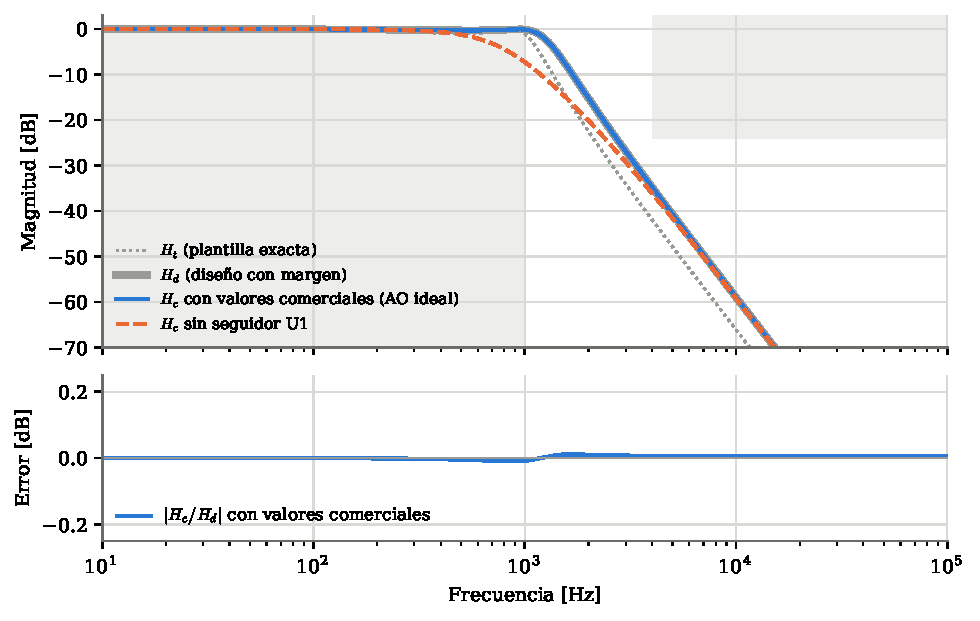
\includegraphics[width=0.92\linewidth]{fig_Hc_vs_Ht}
  \caption{Arriba: $H_t$, $H_d$, $H_c$ con los valores adoptados y $H_c$ sin el seguidor U1. Abajo: error de magnitud de $H_c$ respecto de $H_d$.}
  \label{fig:Hc_vs_Ht}
\end{figure}

Con los valores nominales, el circuito cumple la plantilla con holgura en ambas bandas: $A_{p,\max} = \qty{\vApC}{\decibel}$ frente a
\qty{1}{\decibel}, y $A(\qty{4}{\kilo\hertz}) = \qty{\vAcuatroC}{\decibel}$ frente a \qty{24}{\decibel} (\cref{tab:recalculo,fig:Hc_vs_Ht}).
Repitiendo el Monte Carlo con la realización adoptada, con cada resistencia del par en serie con su propia tolerancia, se obtiene la
\cref{tab:rendimiento} y la \cref{fig:rendimiento}. La tolerancia de los capacitores todavía no está confirmada; si fuera de
$\pm\qty{20}{\percent}$ (cerámicos de uso general), el rendimiento caería a \qty{\vRendVeinte}{\percent}. Por eso se recomiendan capacitores de film
y se verificará su código de tolerancia (J: \qty{5}{\percent}, K: \qty{10}{\percent}, M: \qty{20}{\percent}). El estudio estadístico con LTspice
corresponde al Nivel~II.

\begin{table}[H]
  \centering\small
  \caption{Rendimiento esperado de la realización adoptada ($R$: $\pm\qty{1}{\percent}$, \num{40000} muestras por caso).}
  \label{tab:rendimiento}
  \tabres{tab_rendimiento}
\end{table}

\begin{figure}[H]
  \centering
  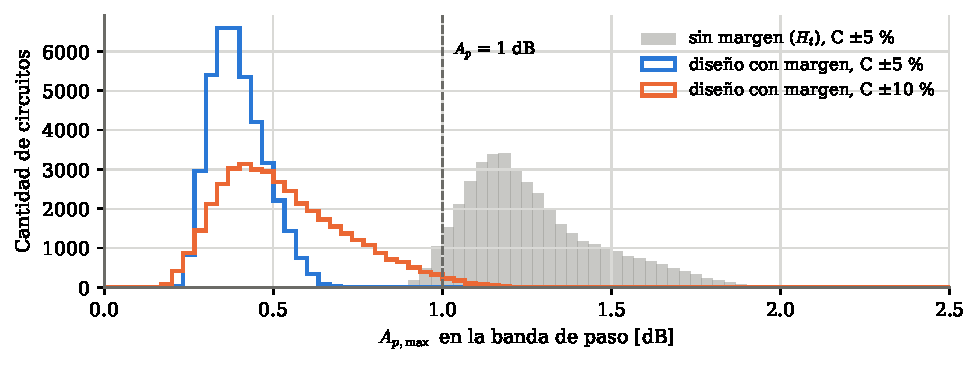
\includegraphics[width=0.9\linewidth]{fig_rendimiento}
  \caption{Distribución de la atenuación máxima en la banda de paso: síntesis sin margen ($H_t$) frente a la realización adoptada ($H_d$).}
  \label{fig:rendimiento}
\end{figure}

\section{Amplificador operacional y lista de materiales}
\label{sec:ao}

\subsection{Datos de hoja técnica}
En el laboratorio hay TL081, TL084, TL071, TL072 y LM358. El TL072 disponible está marcado \textbf{TL072CP}: Texas Instruments, rango comercial
(\qtyrange{0}{70}{\degreeCelsius}) y encapsulado PDIP-8. La \cref{tab:ao} resume los parámetros relevantes según las hojas de datos de
TI~\cite{ti_tl07x,ti_lm358}. La revisión actual de la hoja TL07xx especifica un GBW típico de \qty{5.25}{\mega\hertz} para este encapsulado, mientras
que las revisiones anteriores (y la versión de ST~\cite{st_tl072}) indican entre \qty{3}{\mega\hertz} y \qty{4}{\mega\hertz}. Para no depender de la
revisión del silicio, los cálculos usan \qty{3}{\mega\hertz}.

\begin{table}[H]
  \centering\footnotesize
  \caption{Parámetros de los AO disponibles ($V_{CC} = \qty{\pm 15}{\volt}$, \qty{25}{\degreeCelsius}).}
  \label{tab:ao}
  \tabres{tab_ao}
\end{table}

\subsection{Efecto del GBW finito}
Se repitió el análisis nodal reemplazando ambos AO por $A(s) = \omega_t/s$. La desviación de $\lvert H\rvert$ respecto del caso ideal
(\cref{fig:gbw}) es como máximo de \qty{\vGBWdevTL}{\decibel} hasta \qty{4}{\kilo\hertz} con el TL072CP (con \qty{3}{\mega\hertz}) y de
\qty{\vGBWdevLM}{\decibel} con el LM358. Con $f_0 \approx \qty{1.2}{\kilo\hertz}$ y ganancia unitaria, ambos AO tienen GBW de sobra.

\begin{figure}[H]
  \centering
  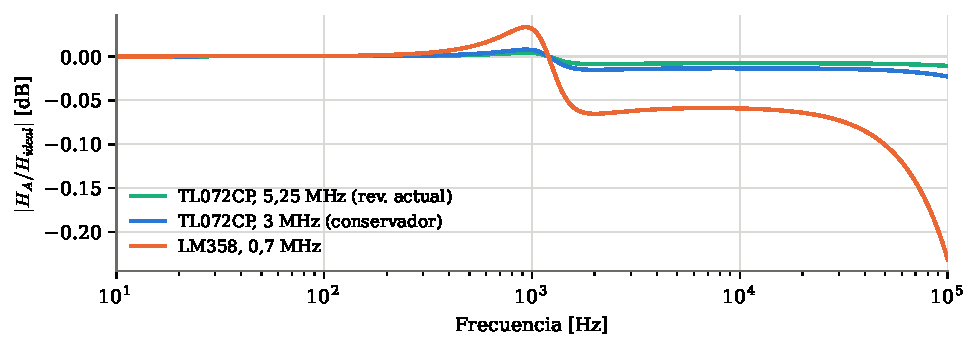
\includegraphics[width=0.85\linewidth]{fig_gbw_finito}
  \caption{Desviación de la respuesta por GBW finito (modelo de un polo), con los valores adoptados.}
  \label{fig:gbw}
\end{figure}

\subsection{Amplitud máxima, slew rate, modo común y carga}
\begin{itemize}
  \item \textbf{Niveles internos.} Con la cascada en el orden elegido, $\max\lvert V_2/V_i\rvert$ y $\max\lvert V_6/V_i\rvert$ valen 1 (en continua) y
        $\max\lvert V_4/V_i\rvert = \num{\vNodoCuatroMax}$ (en \qty{\vNodoCuatroF}{\hertz}). En régimen transitorio, el sobrepico de la respuesta
        al escalón es de \qty{\vSobrepico}{\percent}.
  \item \textbf{Excursión y modo común.} Con alimentación de \qty{\pm 12}{\volt} se adopta un margen de \qty{3}{\volt} a cada riel, que es el mínimo
        de hoja de datos para $R_L = \qty{10}{\kilo\ohm}$. Ese margen cubre también el límite inferior del modo común de la familia TL07x, que no
        llega al riel negativo. Resulta $\lvert v\rvert \le \qty{9}{\volt}$ en todo nodo, y por lo tanto $V_{i,p} \le \qty{\vVinMax}{\volt}$.
  \item \textbf{Slew rate.} Con una entrada senoidal de \qty{\vVinMax}{\volt} de pico en la peor frecuencia, la pendiente máxima es de
        \qty{\vSRUuno}{\volt\per\micro\second} en U1 y de \qty{\vSRUdos}{\volt\per\micro\second} en U2. Ante un escalón de la misma amplitud es de
        \qty{\vSREscalon}{\volt\per\micro\second}. Todos estos valores quedan más de dos órdenes de magnitud por debajo del mínimo garantizado de
        \qty{8}{\volt\per\micro\second}.
  \item \textbf{Carga.} U1 ve como mínimo la impedancia de entrada del Sallen--Key (\qty{\vZminUuno}{\kilo\ohm}); U2, su red de realimentación a
        través de $C_1$ (al menos \qty{\vZminUdos}{\kilo\ohm}) en paralelo con la carga externa del osciloscopio (\qty{1}{\mega\ohm}). Ambas superan
        los \qty{2}{\kilo\ohm} para los que la hoja de datos garantiza la excursión.
\end{itemize}

\subsection{Elección}
Se usa el \textbf{TL072CP} disponible, que aloja U1 y U2 en un solo encapsulado. Tiene entrada JFET con corrientes de polarización de pA
(irrelevantes con resistencias de decenas de k$\Omega$) y bajo ruido. Dos TL081 son un reemplazo directo, uno por etapa. El LM358 cumpliría en GBW y
slew rate para este filtro, pero se descarta por la distorsión de cruce de su etapa de salida, que no tiene polarización clase AB y trabajaría con
señal alterna centrada en \qty{0}{\volt}. También pesan su mayor corriente de polarización y ruido, y que su salida no llega a menos de
\qty{1.5}{\volt} del riel positivo.

Se alimenta con \qty{\pm 12}{\volt} desde la fuente partida del laboratorio, bien por debajo del máximo absoluto de \qty{\pm 18}{\volt}, con un
capacitor cerámico de \qty{100}{\nano\farad} junto a cada pin de alimentación y uno electrolítico de \qty{10}{\micro\farad} por riel. Para las
mediciones se propone una entrada de \qty{1}{\volt} eficaz (aprox. \qty{1.41}{\volt} de pico), con un margen de más de cinco veces respecto de la
saturación. Para medir la banda de rechazo con mejor relación señal/ruido se puede subir hasta unos \qty{5}{\volt} de pico.

\begin{table}[H]
  \centering\footnotesize
  \caption{Lista de materiales. En el filtro se usan capacitores de film (poliéster/MKT) o cerámicos C0G; se evitan los cerámicos de alta constante
  dieléctrica, cuyo valor varía con la tensión y la temperatura. Las resistencias indicadas con «+» se conectan en serie.}
  \label{tab:bom}
  \tabres{tab_bom}
\end{table}

\section{Análisis de sensibilidad}
\label{sec:sensibilidad}

\subsection{Sensibilidades simbólicas}
Se usa la sensibilidad normalizada de un parámetro $P$ respecto de un componente $x$~\cite{daryanani1976,apuntes2026},
\begin{equation}
  S^P_x = \frac{x}{P}\frac{\partial P}{\partial x} = \frac{\partial \ln P}{\partial \ln x}
  \qquad\Longrightarrow\qquad \frac{\Delta P}{P} \approx S^P_x\,\frac{\Delta x}{x}.
  \label{eq:sens_def}
\end{equation}
Se calculó con SymPy sobre las expresiones generales de la \cref{eq:param_circuito}, \emph{antes} de imponer valores o relaciones entre componentes:
\begin{gather}
  S^{\omega_r}_{R_0} = -\frac{R_0}{R_0+R_s},\qquad S^{\omega_r}_{R_s} = -\frac{R_s}{R_0+R_s},\qquad S^{\omega_r}_{C_0} = -1, \label{eq:sens_wr}\\
  S^{\omega_0}_{R_1} = S^{\omega_0}_{R_2} = S^{\omega_0}_{C_1} = S^{\omega_0}_{C_2} = -\frac12, \label{eq:sens_w0}\\
  S^{Q}_{R_1} = -S^{Q}_{R_2} = \frac{R_2-R_1}{2(R_1+R_2)},\qquad S^{Q}_{C_1} = -S^{Q}_{C_2} = \frac12. \label{eq:sens_Q}
\end{gather}
La ganancia en continua es $H(0) = 1$ independientemente de los componentes, de modo que su sensibilidad es nula. No hay resistencias de ganancia del
AO porque ambos trabajan como seguidores. Se verifican además las propiedades de la cátedra: $\sum_R S^{\omega}_R = \sum_C S^{\omega}_C = -1$ para
$\omega_r$ y $\omega_0$ (homogeneidad de grado $-1$ en $R$ y en $C$), y $\sum_R S^Q_R = \sum_C S^Q_C = 0$, porque $Q$ es adimensional y no cambia con un
escaleo de impedancia ni de frecuencia.

La \cref{tab:sensibilidades} evalúa estas expresiones con los componentes adoptados. Para una resistencia formada por dos en serie,
$R = R_a + R_b$, la regla de la cadena da $S^P_{R_a} = S^P_R\,R_a/R$: las resistencias de ajuste (\qty{560}{\ohm}, \qty{3.3}{\kilo\ohm}) aportan
poco, y la tolerancia de \qty{1}{\percent} de cada una se pondera por su fracción del total.

\begin{table}[H]
  \centering\small
  \caption{Sensibilidades normalizadas evaluadas en los componentes adoptados. Abajo, las resistencias individuales de cada par en serie.}
  \label{tab:sensibilidades}
  \tabres{tab_sensibilidades}
\end{table}

Lectura de la tabla:
\begin{itemize}
  \item $\omega_r$ depende prácticamente solo de $R_0$ y $C_0$ ($S \approx -1$). El generador aporta $S^{\omega_r}_{R_s} = \num{-0.0024}$.
  \item $\omega_0$ tiene sensibilidad $-\tfrac12$ respecto de los cuatro elementos del Sallen--Key, cualquiera sea el diseño.
  \item $Q$ depende de los capacitores con $\pm\tfrac12$ y de las resistencias con apenas $\pm\num{0.095}$, gracias a que $R_1 \approx R_2$
        (\cref{sec:sintesis}). \textbf{Los componentes críticos son los capacitores}, que además son los de mayor tolerancia.
\end{itemize}

\subsection{Validación por perturbaciones finitas}
Para validar las expresiones en forma independiente, cada componente se perturbó en $\pm\qty{1}{\percent}$. En cada caso se recalcularon $\omega_r$,
$\omega_0$ y $Q$ a partir de las \emph{raíces del denominador} de $H_c(s)$, evaluado numéricamente, y no de las fórmulas cerradas. Se estimó la
sensibilidad con diferencias unilaterales y con la diferencia central logarítmica
$S \approx [\ln P(x(1+\delta)) - \ln P(x(1-\delta))]/[\ln(1+\delta)-\ln(1-\delta)]$, con $\delta = 0{,}01$ (\cref{tab:validacion_sens}).

\begin{table}[H]
  \centering\small
  \caption{Sensibilidades simbólicas frente a perturbaciones de $\pm\qty{1}{\percent}$ (solo las no nulas).}
  \label{tab:validacion_sens}
  \tabres{tab_validacion_sens}
\end{table}

Las diferencias unilaterales se apartan de la sensibilidad simbólica en el término de segundo orden ($\approx \tfrac12\,\delta\,S(S-1)$ para
$P \propto x^S$, es decir, $\approx \num{0.01}$ para $S = -1$). La diferencia central lo cancela y coincide con la simbólica con un error menor que
\num{\vMaxErrCentral}. Con $\pm\qty{1}{\percent}$ la aproximación lineal es excelente: el cambio porcentual real difiere del predicho en centésimas de
punto porcentual.

\subsection{Efecto del amplificador operacional}
Con $A(s) = \omega_t/s$ en ambos AO y GBW de \qty{3}{\mega\hertz}, el GBW finito desplaza $f_0$ en \qty{\vDfoGBW}{\percent} y $Q$ en
\qty{\vDQGBW}{\percent}, mientras que $\omega_r$ no se modifica. La sensibilidad de $Q$ respecto del GBW es $S^Q_{\mathrm{GBW}} = \num{\vSQGBW}$: una
variación de \qty{50}{\percent} del GBW entre unidades o revisiones del TL072 cambiaría $Q$ en menos de \qty{0.04}{\percent}. El AO no es un
elemento crítico de este diseño.

\subsection{Sensibilidad de la magnitud y dispersión esperada}
La parte real de la sensibilidad de la función, $S^{|H|}_x(\omega) = \mathrm{Re}\{(x/H)\,\partial H/\partial x\}$, indica cuánto cambia la magnitud
en cada frecuencia (\cref{fig:sens_magnitud}). En la banda de paso baja todas son prácticamente nulas, porque $H(0) = 1$ por construcción. Cerca del
borde, en \qty{1}{\kilo\hertz}, dominan $R_0$ y $C_0$ ($\approx \num{-0.62}$) y $C_1$ ($\num{\vSHmilCuno}$). En la banda de rechazo todas tienden a
$-1$, que es la sensibilidad de un pasabajos de orden~3 por encima de sus polos: la atenuación crece \qty{0.087}{\decibel} por cada
\qty{1}{\percent} de aumento de cualquier $R$ o $C$.

\begin{figure}[H]
  \centering
  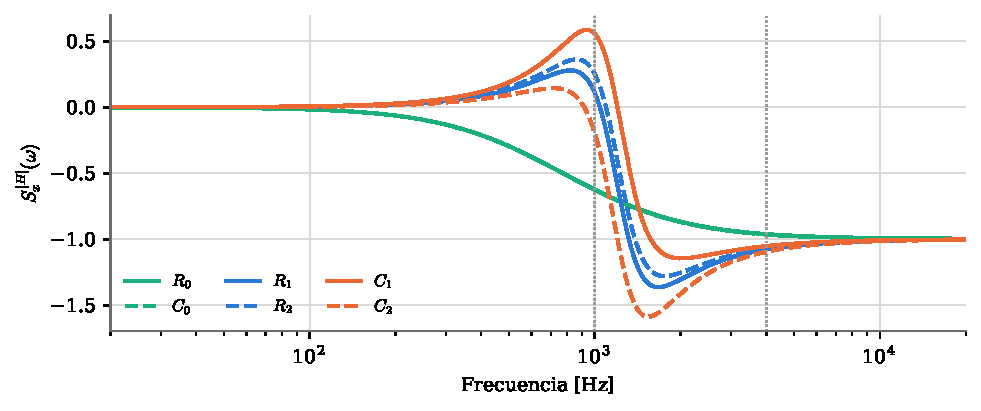
\includegraphics[width=0.9\linewidth]{fig_sens_magnitud}
  \caption{Sensibilidad de la magnitud respecto de cada componente. Las líneas punteadas son los bordes de la plantilla (\qty{1}{\kilo\hertz} y
  \qty{4}{\kilo\hertz}).}
  \label{fig:sens_magnitud}
\end{figure}

Con variaciones independientes y uniformes de semiancho $t_x$ ($\sigma_x/x = t_x/\sqrt3$), la desviación estándar de la magnitud en dB es
\begin{equation}
  \sigma_{|H|,\mathrm{dB}}(\omega) \approx \frac{20}{\ln 10}\sqrt{\sum_x \left(S^{|H|}_x(\omega)\right)^2 \left(\frac{t_x}{\sqrt3}\right)^2}.
\end{equation}
En la banda de paso, el máximo está en el borde de \qty{1}{\kilo\hertz}: \qty{\vSigCincoPaso}{\decibel} con capacitores de
$\pm\qty{5}{\percent}$ y \qty{\vSigDiezPaso}{\decibel} con $\pm\qty{10}{\percent}$ (\cref{fig:banda_dispersion}). Con $\pm 2\sigma$ la banda queda
dentro de la plantilla para capacitores de $\pm\qty{5}{\percent}$ y apenas la toca para $\pm\qty{10}{\percent}$, en coincidencia con el
rendimiento estimado en la \cref{sec:margen}. A \qty{4}{\kilo\hertz}, la dispersión ($\sigma \le \qty{\vSigDiezCuatro}{\decibel}$) es despreciable
frente a los \qty{10.7}{\decibel} de margen.

\begin{figure}[H]
  \centering
  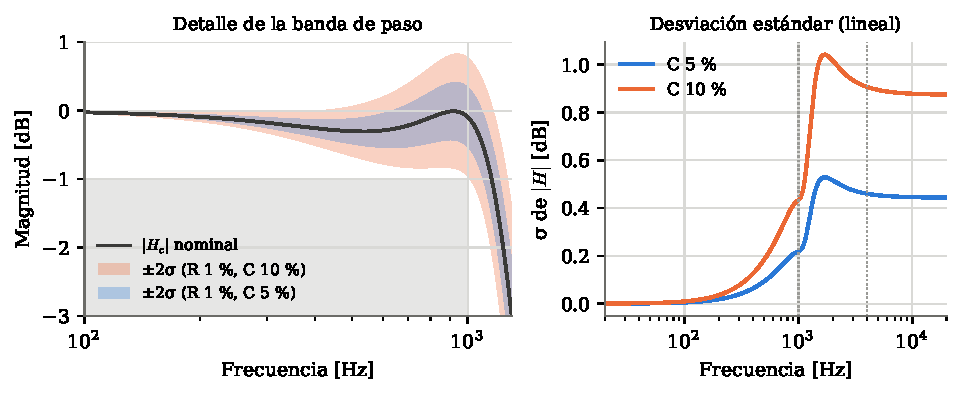
\includegraphics[width=\linewidth]{fig_banda_dispersion}
  \caption{Izquierda: magnitud nominal y banda $\pm 2\sigma$ en la banda de paso (zona gris: región prohibida). Derecha: desviación estándar de
  $|H|$ en función de la frecuencia.}
  \label{fig:banda_dispersion}
\end{figure}

\subsection{Predicción lineal de la dispersión de los parámetros}
La predicción de primer orden para variables independientes, $(\sigma_P/P)^2 \approx \sum_x (S^P_x)^2(\sigma_x/x)^2$, se contrastó con un Monte
Carlo de \num{100000} muestras sobre las expresiones exactas (\cref{tab:dispersion_lineal}). La coincidencia es muy buena: la desviación estándar
lineal difiere de la muestral en menos de \qty{1}{\percent} relativo. El sesgo de la media es pequeño y crece con la tolerancia (es un efecto de
segundo orden: $\omega \propto x^{-1}$ o $x^{-1/2}$ es convexa). El contraste con el Monte Carlo de LTspice forma parte del Nivel~II.

\begin{table}[H]
  \centering\small
  \caption{Dispersión relativa de $\omega_r$, $\omega_0$ y $Q$: predicción lineal frente a Monte Carlo ($R$: $\pm\qty{1}{\percent}$, uniforme).}
  \label{tab:dispersion_lineal}
  \tabres{tab_dispersion_lineal}
\end{table}

\section{Simulación en LTspice}
\label{sec:ltspice}

\subsection{Netlists}
Los netlists se generan desde el notebook~03 a partir de los mismos valores de componentes que usa el resto del informe
(\texttt{resultados/componentes.json}), de modo que no hay transcripción manual. Respetan la numeración de nodos de la \cref{fig:esquema} y modelan
cada resistencia en serie como dos elementos (nodos intermedios 11, 31 y 41). Se compara la cadena completa de modelos:
\begin{enumerate}
  \item \textbf{Respuesta ideal}: función de diseño $H_d(s)$ (SciPy).
  \item \textbf{Respuesta circuital ideal}: $H_c(s)$ con AO ideales (SymPy) y el mismo circuito en LTspice con AO ideal (fuente controlada de
        ganancia $10^6$).
  \item \textbf{AO lineal de un polo} ($A_0 = 2\cdot10^5$, GBW de \qty{3}{\mega\hertz}). Es un \emph{modelo pedagógico}, que solo aísla el efecto
        del GBW y no constituye una validación comercial.
  \item \textbf{Modelo del fabricante}: macromodelo PSpice del TL072 de Texas Instruments (SLOJ067), alimentado con \qty{\pm 12}{\volt}. Incluye
        etapa de entrada JFET, limitación de slew rate, impedancia de salida y saturación.
\end{enumerate}

\begin{table}[H]
  \centering\small
  \caption{Netlists entregados (carpeta \texttt{ltspice/}).}
  \label{tab:netlists}
  \begin{tabular}{@{}lll@{}}
    \toprule
    Archivo & AO & Análisis \\
    \midrule
    \texttt{filtro\_ideal\_ac.cir}       & ideal (VCVS)            & AC, \qty{10}{\hertz}--\qty{100}{\kilo\hertz} \\
    \texttt{filtro\_lineal\_ac.cir}      & lineal de un polo       & AC \\
    \texttt{filtro\_TL072\_ac.cir}       & TL072 (TI)              & AC \\
    \texttt{filtro\_TL072\_tran.cir}     & TL072 (TI)              & senoidal \qty{1}{\volt} eficaz a \qty{200}{\hertz}, \qty{1}{\kilo\hertz} y \qty{4}{\kilo\hertz} \\
    \texttt{filtro\_TL072\_escalon.cir}  & TL072 (TI)              & escalón de \qty{1}{\volt} \\
    \texttt{filtro\_TL072\_gran\_senal.cir} & TL072 (TI)           & senoidal de 4, 8 y \qty{11}{\volt} pico a \qty{936}{\hertz} \\
    \bottomrule
  \end{tabular}
\end{table}

Cada netlist incluye mediciones automáticas (\texttt{.meas}). En el análisis AC se miden la ganancia máxima y mínima en la banda de paso, $|H|$ en
\qty{1}{\kilo\hertz} y en \qty{4}{\kilo\hertz}, la frecuencia de \qty{-3}{\decibel} y el nivel máximo del nodo~4. En los transitorios se miden la
amplitud pico a pico de entrada y de salida, la ganancia, las tensiones máximas en las salidas de los AO y el sobrepico ante el escalón. El ensayo de
gran señal se hace a \qty{936}{\hertz}, la frecuencia de mayor nivel interno, con \qty{4}{\volt} y \qty{8}{\volt} de pico (dentro del límite de
\qty{\vVinMax}{\volt} calculado en la \cref{sec:ao}) y con \qty{11}{\volt} de pico, para observar el recorte. El listado siguiente corresponde al
análisis AC con el modelo del fabricante:

\VerbatimInput[fontsize=\footnotesize,frame=single,framesep=2mm]{\ltsdir/filtro_TL072_ac.cir}

\subsection{Verificación de los netlists}
Antes de usar LTspice, los netlists se verificaron con un solver de análisis nodal modificado (MNA) escrito en NumPy. El solver lee el netlist
(resistencias, capacitores, fuentes de tensión, fuentes controladas y \texttt{.param}), resuelve el análisis AC y compara el resultado con la
$H_c(s)$ de SymPy. Para el netlist con AO ideal, el error relativo máximo entre \qty{10}{\hertz} y \qty{100}{\kilo\hertz} es de
\num{\vErrMNA}, que es del orden de $1/A$ para una ganancia de lazo abierto de $10^6$. Esto confirma que la topología, la numeración de nodos y los
valores del netlist coinciden con el circuito analizado.

\subsection{Resultados}
Las simulaciones se corrieron con LTspice 24.1.10 para Windows. Con el macromodelo de TI, la búsqueda del punto de operación no converge por
iteración directa ni por \emph{Gmin stepping}, y LTspice la resuelve por \emph{source stepping}, lo que es habitual con estos macromodelos y no
afecta el resultado. El macromodelo (TI, 1989) tiene un GBW de $g_A/(2\pi C_2) = \qty{282.8}{\micro\siemens}/(2\pi\cdot\qty{15}{\pico\farad})
\approx \qty{3}{\mega\hertz}$, el mismo valor adoptado en los cálculos.

\subsubsection{Respuesta en frecuencia}
La \cref{tab:ltspice_ac} compara las mediciones automáticas de LTspice con el cálculo en Python y la \cref{fig:ltspice_ac} superpone las curvas.
Con AO ideal, LTspice reproduce $H_c(s)$ con una diferencia menor que \qty{1e-4}{\decibel} en magnitud y \ang{2e-4} en fase, lo que confirma el
circuito, el netlist y la derivación simbólica. Con el modelo del TL072, la diferencia respecto de $H_c$ es de \qty{\vTLdevCuatrok}{\decibel} y
\ang{\vTLfaseCuatrok} como máximo hasta \qty{4}{\kilo\hertz}, prácticamente igual a la del AO lineal de un polo con el mismo GBW: en la banda de
interés, el único efecto apreciable del AO real es su GBW finito, en coincidencia con la \cref{sec:ao}. El filtro simulado con el modelo de
fabricante cumple la plantilla con el mismo margen que el nominal.

\begin{table}[H]
  \centering\small
  \caption{Mediciones \texttt{.meas} de LTspice frente al cálculo en Python con los mismos componentes.}
  \label{tab:ltspice_ac}
  \resizebox{\linewidth}{!}{\tabres{tab_ltspice_ac}}
\end{table}

\begin{figure}[H]
  \centering
  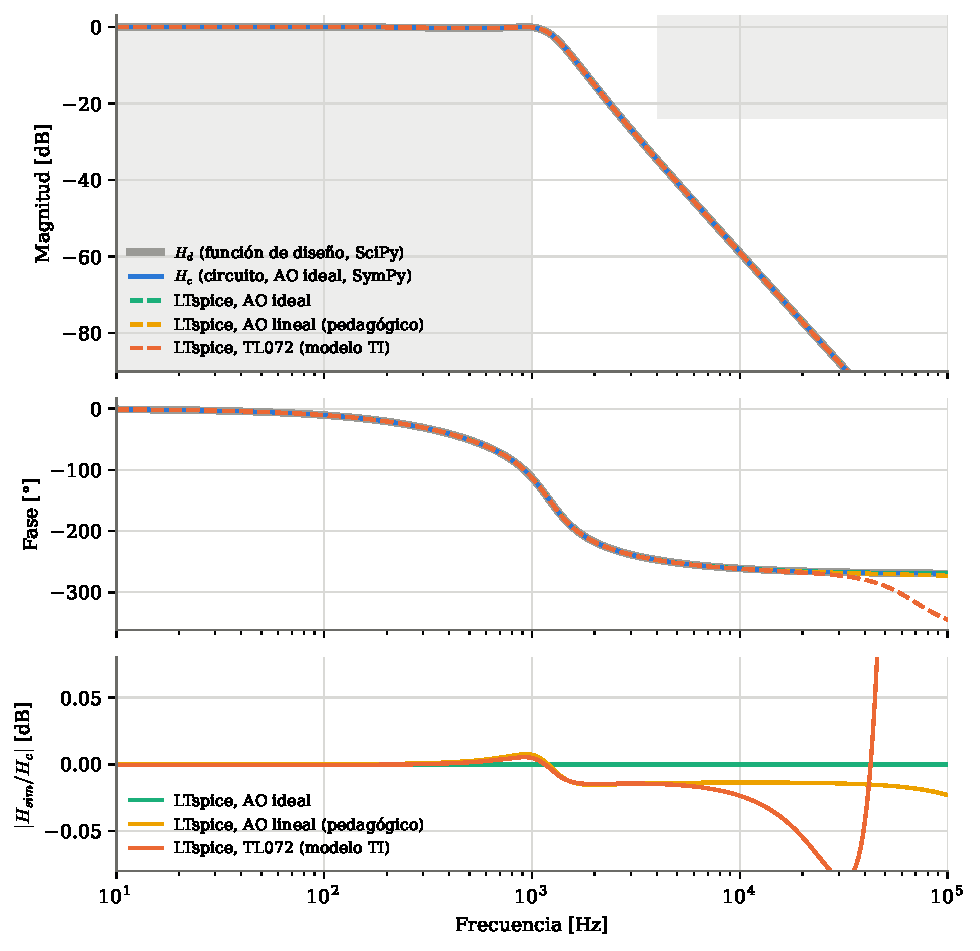
\includegraphics[width=0.92\linewidth]{fig_ltspice_ac}
  \caption{Respuesta en frecuencia: función de diseño, circuito ideal (SymPy) y simulaciones de LTspice. Abajo, diferencia de magnitud respecto de
  $H_c$ (la desviación del TL072 por encima de \qty{20}{\kilo\hertz} se analiza en la \cref{fig:ltspice_altafrec}).}
  \label{fig:ltspice_ac}
\end{figure}

\paragraph{Fuga en alta frecuencia.} Por encima de unos \qty{40}{\kilo\hertz}, el modelo del TL072 se aparta del circuito ideal
(\cref{fig:ltspice_altafrec}). A \qty{100}{\kilo\hertz} atenúa \qty{\vTLAcienk}{\decibel} en lugar de \qty{\vIdAcienk}{\decibel}, es decir,
\qty{\vTLdevCienk}{\decibel} menos. Es la limitación conocida del Sallen--Key de ganancia unitaria. A esas frecuencias $C_1$ y $C_2$ son casi
cortocircuitos, el nodo~4 queda unido a la salida y la corriente que entra por $R_1$ desde U1 se inyecta en la salida de U2. Con un AO real, la
impedancia de salida en lazo cerrado $Z_o \approx r_o/(1+A(j\omega))$ crece con la frecuencia y aparece un camino directo
$V_o \approx V_3\,Z_o/R_1$. Con $r_o \approx \qty{300}{\ohm}$ (macromodelo) y un GBW de \qty{3}{\mega\hertz}, esta estimación da
\qty{\vEstAcienk}{\decibel} a \qty{100}{\kilo\hertz}, del mismo orden que la simulación. El modelo lineal sin impedancia de salida no reproduce el
efecto. No compromete la plantilla, que exige \qty{24}{\decibel}, pero limita la atenuación última del filtro y debe tenerse en cuenta al medir la
banda de rechazo lejana.

\begin{figure}[H]
  \centering
  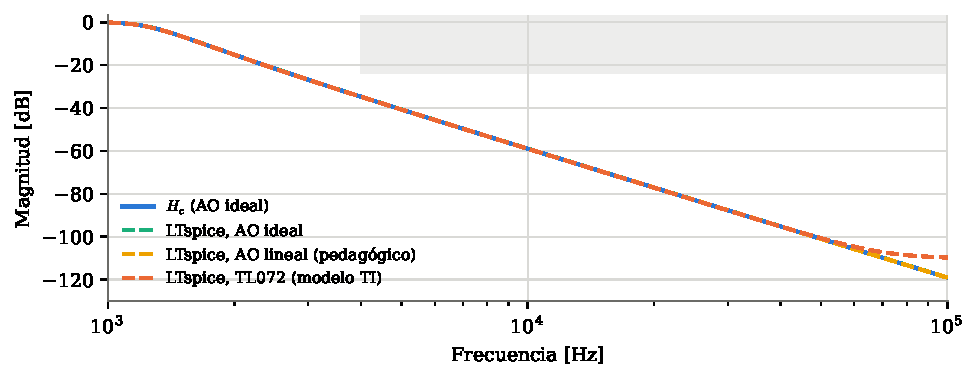
\includegraphics[width=0.85\linewidth]{fig_ltspice_altafrec}
  \caption{Banda de rechazo hasta \qty{100}{\kilo\hertz}: fuga del Sallen--Key de ganancia unitaria con el modelo del TL072.}
  \label{fig:ltspice_altafrec}
\end{figure}

\subsubsection{Transitorio senoidal}
Con una entrada senoidal de \qty{1}{\volt} eficaz a \qty{200}{\hertz}, \qty{1}{\kilo\hertz} y \qty{4}{\kilo\hertz} (\cref{fig:ltspice_tran}),
la ganancia y el desfase en régimen permanente se obtuvieron ajustando por mínimos cuadrados un seno de frecuencia conocida a la entrada y a la salida
entre \qty{20}{\milli\second} y \qty{30}{\milli\second}. Coinciden con $H_c(j\omega)$ dentro de \qty{0.02}{\decibel} y \ang{0.2}
(\cref{tab:ltspice_tran}). Las salidas de los AO no se acercan a la saturación.

\begin{figure}[H]
  \centering
  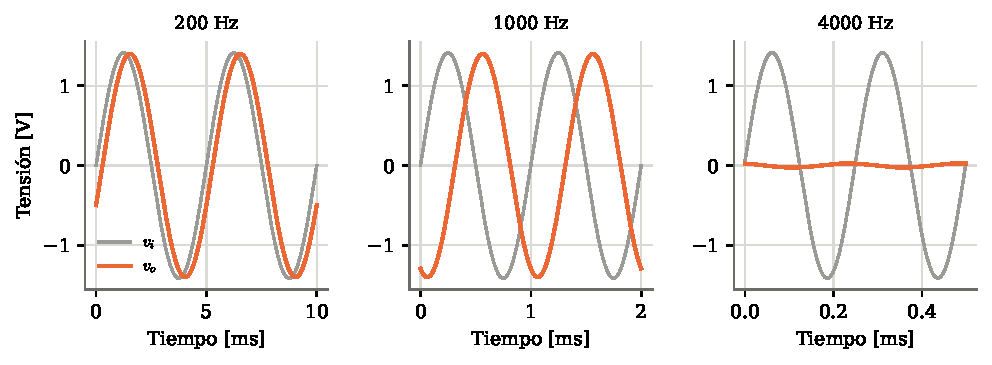
\includegraphics[width=\linewidth]{fig_ltspice_tran}
  \caption{Transitorio con el modelo del TL072: entrada y salida en régimen permanente (dos períodos).}
  \label{fig:ltspice_tran}
\end{figure}

\begin{table}[H]
  \centering\small
  \caption{Ganancia y fase obtenidas del transitorio de LTspice (TL072) frente a $H_c(j\omega)$.}
  \label{tab:ltspice_tran}
  \resizebox{\linewidth}{!}{\tabres{tab_ltspice_tran}}
\end{table}

\subsubsection{Respuesta al escalón}
Ante un escalón de \qty{1}{\volt}, la salida simulada con el TL072 sigue a la respuesta calculada de $H_c$ (\cref{fig:ltspice_escalon}). LTspice mide
un sobrepico de \qty{\vSobrepicoLT}{\percent}, frente a \qty{\vSobrepicoPy}{\percent} de $H_c$, con valor final \qty{1.000}{\volt}. En una primera
corrida se había obtenido \qty{9.99}{\percent}: LTspice comprime por defecto las formas de onda (\texttt{plotwinsize}) y había guardado solo 43
puntos, y las mediciones \texttt{.meas} se evalúan sobre esos datos comprimidos. Con \texttt{.options plotwinsize=0} se guardan los
\num{\vPuntosEscalon}~puntos calculados y la diferencia con el cálculo se reduce a centésimas de punto porcentual. Por eso todos los netlists de
transitorio incluyen esa opción.

\begin{figure}[H]
  \centering
  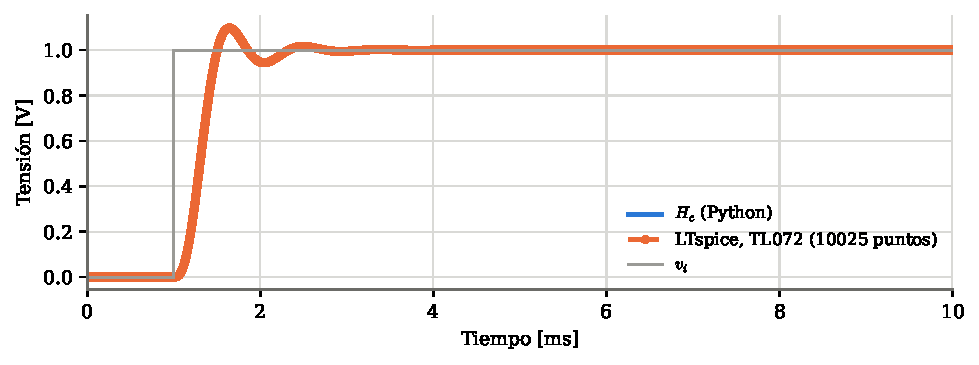
\includegraphics[width=0.9\linewidth]{fig_ltspice_escalon}
  \caption{Respuesta al escalón de \qty{1}{\volt}: $H_c$ (Python) y LTspice con el modelo del TL072.}
  \label{fig:ltspice_escalon}
\end{figure}

\subsubsection{Gran señal}
A \qty{936}{\hertz}, la frecuencia de mayor nivel interno, la salida alcanza \qty{\vGSmaxCuatro}{\volt} y \qty{\vGSmaxOcho}{\volt} de pico con
entradas de \qty{4}{\volt} y \qty{8}{\volt}, sin distorsión visible. Con \qty{11}{\volt} de pico recorta en \qty{\vGSmaxOnce}{\volt} y
\qty{\vGSminOnce}{\volt} (\cref{fig:ltspice_gran_senal}), mientras U1 llega solo a \qty{\vGSUunoOnce}{\volt} porque la etapa~1 ya atenúa a esa
frecuencia: la etapa que satura es U2. La excursión del modelo con \qty{\pm 12}{\volt} es de unos \qty{1.5}{\volt} por debajo de cada riel, de modo que
el límite de \qty{\pm 9}{\volt} adoptado en la \cref{sec:ao} es conservador y la amplitud propuesta para las mediciones (\qty{1}{\volt} eficaz)
tiene un margen de más de siete veces.

\begin{figure}[H]
  \centering
  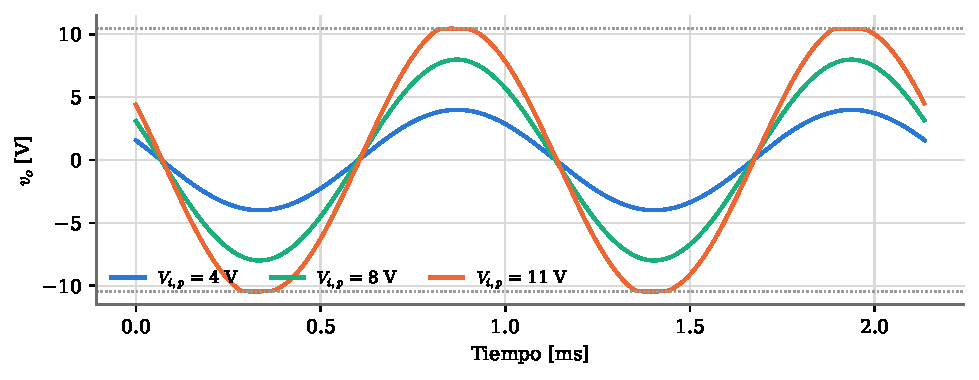
\includegraphics[width=0.9\linewidth]{fig_ltspice_gran_senal}
  \caption{Ensayo de gran señal a \qty{936}{\hertz} con el modelo del TL072 y alimentación de \qty{\pm 12}{\volt}.}
  \label{fig:ltspice_gran_senal}
\end{figure}

\section{Implementación y mediciones}
\label{sec:mediciones}

\subsection{Implementación}
El filtro se monta en una placa de circuito impreso diseñada en EasyEDA. La asignación de pines del TL072CP (DIP-8) es la siguiente:
\begin{itemize}
  \item \textbf{U1 (mitad A):} pin~3 ($+$) al nodo~2; pines~1 (salida) y~2 ($-$) unidos, nodo~3.
  \item \textbf{U2 (mitad B):} pin~5 ($+$) al nodo~5; pines~7 (salida) y~6 ($-$) unidos, nodo~6.
  \item \textbf{Alimentación:} pin~8 a $+\qty{12}{\volt}$ y pin~4 a $-\qty{12}{\volt}$.
\end{itemize}
Criterios de diseño de la placa:
\begin{itemize}
  \item \textbf{Desacople:} un capacitor cerámico de \qty{100}{\nano\farad} lo más cerca posible de los pines~8 y~4, a masa, y uno electrolítico de
        \qty{10}{\micro\farad} por riel junto al conector de alimentación.
  \item \textbf{Masa:} plano de masa en la cara inferior. Las corrientes de alimentación y de desacople no deben circular por el tramo de masa de la
        entrada ni por el de la salida.
  \item \textbf{Nodos de alta impedancia} (2, 4 y 5): pistas cortas. $C_1$, $C_2$ y $R_2$ quedan junto a U2. La pista de salida no corre paralela a la
        de entrada, para no agregar un acople capacitivo que degrade la banda de rechazo, ya limitada en alta frecuencia por la fuga del Sallen--Key
        (\cref{sec:ltspice}).
  \item \textbf{Resistencias en serie:} huellas para dos resistencias por posición ($R_0$, $R_1$, $R_2$).
  \item \textbf{Conexiones y puntos de prueba:} entrada y salida en extremos opuestos de la placa (BNC o borneras con masa propia), puntos de prueba en
        los nodos 1, 3, 4 y 6, y lazos de masa para las puntas del osciloscopio.
  \item \textbf{Alimentación:} bornera de tres terminales ($+12$, GND, $-12$) con serigrafía clara. Opcionalmente, diodos en serie por riel como
        protección contra inversión de polaridad: la caída de unos \qty{0.7}{\volt} es admisible por el margen de excursión
        (\cref{sec:ao}).
  \item \textbf{Zócalo} para el TL072, de modo de poder reemplazarlo por dos TL081 o repetir mediciones con otra unidad.
\end{itemize}

\subsection{Procedimiento de medición}
\paragraph{Antes de energizar.} Se verifica la placa contra el esquema (orientación del integrado, alimentación y desacople) y la ausencia de
cortocircuitos entre rieles y masa. Se miden con multímetro las resistencias (cada par en serie como un total) y se registra el código de tolerancia de cada capacitor. La fuente
partida se ajusta a $\pm\qty{12}{\volt}$ con límite de corriente de \qty{50}{\milli\ampere} antes de conectarla; el consumo esperado es de unos
\qty{3}{\milli\ampere} por riel. Con la entrada a masa se mide la tensión continua de salida (offset).

\paragraph{Conexión.} El canal~1 del osciloscopio se conecta al borne de entrada del filtro (nodo~1) y el canal~2 a la salida (nodo~6), con puntas
$\times10$ ($\qty{10}{\mega\ohm}\parallel\approx\qty{15}{\pico\farad}$), acoplamiento DC, límite de ancho de banda de \qty{20}{\mega\hertz} y
promediado. Al tomar la referencia en el nodo~1, la magnitud medida es $V_6/V_1$: la resistencia interna del generador no interviene y el modelo de
comparación es $H_c$ con $R_s = 0$.

\paragraph{Barrido.} La medición se hizo finalmente con el modo \emph{Bode} del osciloscopio, que automatiza el barrido
(ver resultados). El plan manual, que queda como respaldo y para repetir puntos aislados, mide 34 frecuencias entre \qty{20}{\hertz} y \qty{20}{\kilo\hertz}, más densas entre \qty{700}{\hertz} y
\qty{1.5}{\kilo\hertz} (rizado, borde de paso y transición). La amplitud de entrada es de \qty{1}{\volt} eficaz hasta \qty{2}{\kilo\hertz} y de
\qty{3}{\volt} eficaces desde \qty{2.5}{\kilo\hertz}, para mejorar la relación señal/ruido donde la salida es pequeña: a esas frecuencias la
etapa~1 ya atenúa y ningún nodo se acerca a la saturación. En cada punto se miden $V_{1,\mathrm{rms}}$, $V_{6,\mathrm{rms}}$ y el retardo $\Delta t$
entre cruces por cero ascendentes. La fase es $\varphi = -360^\circ f\,\Delta t$, con $\Delta t > 0$ si la salida atrasa. Como el osciloscopio
entrega $\varphi$ módulo \ang{360} y la fase real llega a \ang{-265}, el giro se resuelve con la fase esperada; esto solo elige el número entero de
vueltas, no ajusta el dato. La planilla del repositorio incluye, para cada frecuencia, la ganancia, la salida, la fase y el $\Delta t$ esperados,
que sirven para elegir escalas y detectar errores durante la medición.

\paragraph{Ensayos adicionales.} Respuesta a una onda cuadrada de \qty{50}{\hertz} (sobrepico esperado de \qty{\vSobrepicoPy}{\percent}) y, si el
generador lo permite, ensayo de gran señal a \qty{936}{\hertz} hasta observar el recorte (esperado: $\pm\qty{10.4}{\volt}$ con $\pm\qty{12}{\volt}$,
\cref{sec:ltspice}).

\subsection{Procesamiento e incertidumbre}
Las mediciones se procesan con el notebook~04:
\begin{itemize}
  \item \textbf{Ganancia:} $G = 20\log_{10}(V_6/V_1)$. Con una precisión vertical relativa $a$ por canal (distribución rectangular),
        $u(G) \approx \frac{20}{\ln 10}\sqrt2\,a/\sqrt3$. Con $a = \qty{3}{\percent}$ resulta \qty{0.21}{\decibel}; es una cota conservadora, porque
        parte del error es común a ambos canales y se cancela en el cociente.
  \item \textbf{Fase:} $u(\varphi) = \ang{1}$. Antes de medir se corre un Bode con los dos canales en el mismo punto; lo que el instrumento mide ahí
        es su propio error entre canales, y se descuenta de todas las mediciones de la sesión.
  \item \textbf{Parámetros característicos:} se obtienen $A_{p,\max}$, $|H(\qty{1}{\kilo\hertz})|$, $|H(\qty{4}{\kilo\hertz})|$ y la frecuencia de
        \qty{-3}{\decibel} interpolando la medición. Además se ajustan $f_r$, $f_0$, $Q$ y una ganancia $K$ por mínimos cuadrados no lineales sobre
        la ganancia y la fase de los puntos con la salida a no más de \qty{30}{\decibel} por debajo de la de continua; la incertidumbre de los
        parámetros combina la covarianza del ajuste, $(J^TJ)^{-1}$ escalada por el $\chi^2$ reducido, con la variación por la elección de esa
        banda.
  \item \textbf{Capacitores:} como no se dispone de un medidor LCR, sus valores reales se estiman en forma indirecta invirtiendo la
        \cref{eq:param_circuito} con los parámetros ajustados y las resistencias medidas: $C_0 = 1/(\omega_rR_0)$,
        $C_1/C_2 = Q^2(R_1+R_2)^2/(R_1R_2)$ y $C_1C_2 = 1/(\omega_0^2R_1R_2)$. El procedimiento se validó con datos sintéticos, con desvíos
        impuestos de $+4$, $-3$ y $+\qty{6}{\percent}$ y ruido de medición realista, que se recuperaron con un error menor que
        \num{0.15} puntos porcentuales. Esos datos sintéticos no forman parte del repositorio ni de los resultados.
  \item \textbf{Retardo de grupo:} se estima de la fase medida como $-\Delta\varphi/\Delta\omega$ entre frecuencias separadas unas 0,1~década y se
        compara con el del modelo nominal y el del modelo ajustado.
\end{itemize}

\subsection{Resultados}
\IfFileExists{\resdir/valores_nb04.tex}{%
\paragraph{Condiciones.} Instrumental: osciloscopio Rigol MSO5074, generador de funciones Rigol DG1022, multímetro UNI-T UT61D+ y fuente
OWON ODP3063 (alimentación medida: $\pm\qty{\mVcc}{\volt}$). La respuesta en frecuencia se midió con el modo \emph{Bode} del osciloscopio,
con barrido logarítmico de \qty{10}{\hertz} a \qty{100}{\kilo\hertz} (\mNfrec{} frecuencias, 50 por década) y \qty{5}{\volt} pico a pico, con puntas
$\times10$ y en la misma sesión que el Nivel~III (\cref{sec:nivel3}). La calibración de canales descrita arriba mostró errores entre canales de a lo
sumo \qty{0.02}{\decibel} y \ang{0.4} hasta \qty{20}{\kilo\hertz}, que se descuentan. La respuesta al escalón se midió con una onda cuadrada de
\qty{2}{\volt} pico a pico y \qty{50}{\hertz}. Los archivos exportados por el instrumento se guardan sin modificar en
\texttt{mediciones/nivel3/}, junto con las capturas de pantalla. Las resistencias
medidas (cada par en serie como un total) son $R_0 = \qty{\mRceroMed}{\kilo\ohm}$, $R_1 = \qty{\mRunoMed}{\kilo\ohm}$ y
$R_2 = \qty{\mRdosMed}{\kilo\ohm}$, con desvíos de \qr{1}{\mDRcero}{\percent}, \qr{1}{\mDRuno}{\percent} y \qr{1}{\mDRdos}{\percent} respecto de los
valores nominales, compatibles con la tolerancia de \qty{1}{\percent} de cada resistencia más la precisión del multímetro. Con la entrada a masa,
la tensión continua de salida es de \qty{\mOffset}{\milli\volt}: la suma de las tensiones de offset de los dos seguidores, dentro de lo esperable para
el TL072 (\qty{3}{\milli\volt} típicos y \qty{10}{\milli\volt} máximos por AO).

\paragraph{Cumplimiento de la plantilla.} El filtro construido cumple la plantilla (\cref{tab:parametros_medicion,fig:mediciones_bode}). La
atenuación máxima en la banda de paso es de \qr{2}{\mApMaxMed}{\decibel}, por debajo de \qty{1}{\decibel}, y se da en el borde de \qty{1}{\kilo\hertz}.
A \qty{4}{\kilo\hertz} la atenuación es de \qr{1}{\mAcuatrokMed}{\decibel}, con más de \qty{11}{\decibel} de margen sobre los \qty{24}{\decibel}
exigidos. La frecuencia de \qty{-3}{\decibel} es de \qr{0}{\mFtresdBMed}{\hertz}, frente a \qr{0}{\mFtresdBNom}{\hertz} del diseño nominal.

\begin{table}[H]
  \centering\small
  \caption{Parámetros característicos medidos frente a la plantilla y al diseño nominal ($H_c$ con $R_s = 0$, porque se mide $V_6/V_1$).}
  \label{tab:parametros_medicion}
  \tabres{tab_parametros_medicion}
\end{table}

\begin{figure}[H]
  \centering
  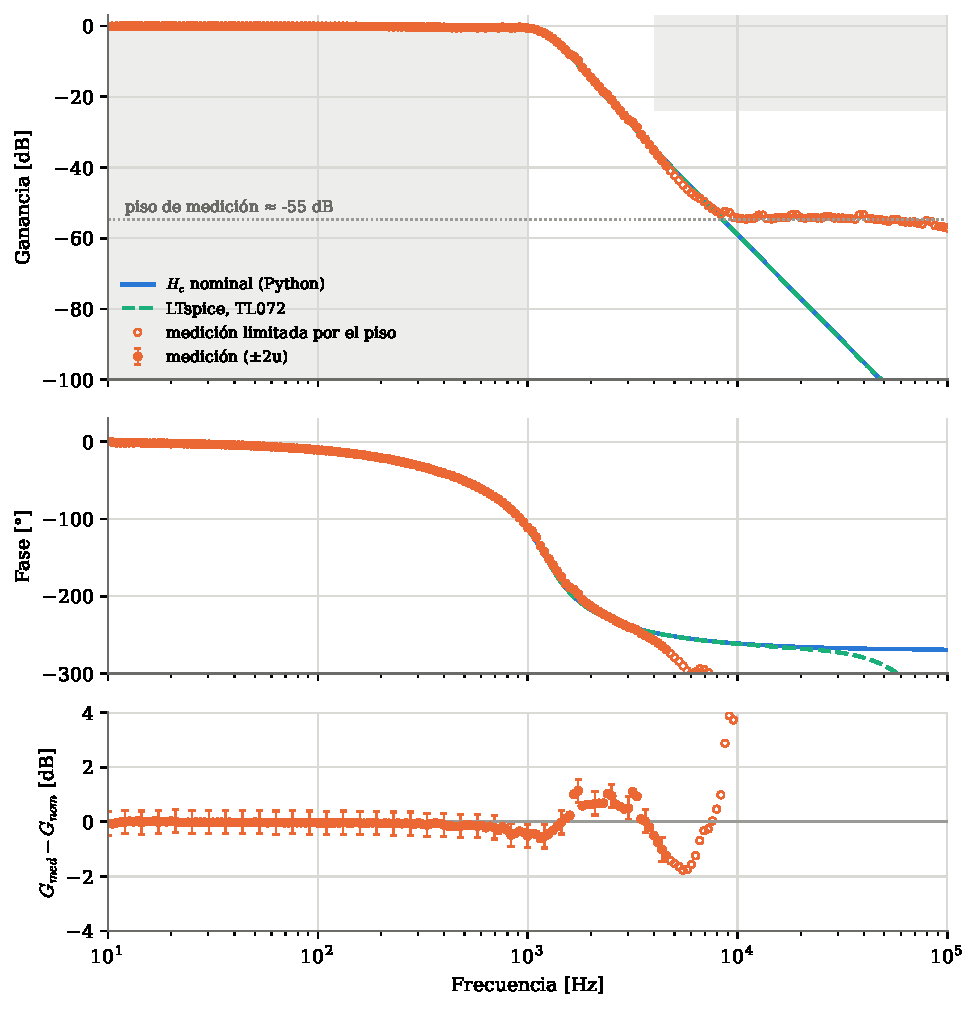
\includegraphics[width=0.95\linewidth]{fig_mediciones_bode}
  \caption{Respuesta medida (modo Bode, Rigol MSO5074) frente al modelo nominal y a LTspice con el TL072. Los puntos huecos están limitados por el
  piso de medición y no se usan en el análisis. Abajo: diferencia entre la ganancia medida y la nominal.}
  \label{fig:mediciones_bode}
\end{figure}

\paragraph{Piso de medición.} Por encima de unos \qty{9}{\kilo\hertz}, la ganancia medida se estabiliza en \qr{0}{\mPiso}{\decibel}, mientras que
el filtro debería seguir cayendo (\qty{-59}{\decibel} a \qty{10}{\kilo\hertz} y \qty{-77}{\decibel} a \qty{20}{\kilo\hertz}). Es el límite del
sistema de medición, no del filtro: con \qty{5}{\volt} pico a pico de entrada, \qty{-54}{\decibel} equivale a unos \qty{2}{\milli\volt} pico a pico,
del orden del ruido del canal visible en la captura (\qty{10}{\milli\volt\per div}). Entre \qty{4.5}{\kilo\hertz} y \qty{9}{\kilo\hertz} la
medición ya está perturbada por la suma de ese piso con la señal. Por eso solo se consideran válidos los puntos que quedan al menos
\qty{15}{\decibel} por encima del piso: \mNValidos{} puntos, hasta \qr{0}{\mFMaxValido}{\hertz}. Medir más allá requiere más amplitud de entrada,
promediado o un instrumento con más rango dinámico, y aun así la atenuación última queda limitada por la fuga del Sallen--Key (\cref{sec:ltspice}).

\paragraph{Ajuste del modelo.} Ajustando $f_r$, $f_0$, $Q$ y $K$ a la ganancia y la fase de los puntos con la salida a no más de
\qty{30}{\decibel} por debajo de la de continua (hasta \qr{0}{\mFMaxAjuste}{\hertz}) se obtiene la \cref{tab:ajuste_medicion}, con $\chi^2$ reducido
de \nr{2}{\mChiCuadRed}: el modelo describe la medición dentro de la incertidumbre supuesta, que es conservadora (\cref{fig:mediciones_paso}). La
fase es la que fija $f_r$; con la ganancia sola, $f_r$ y $Q$ están fuertemente correlacionados. La banda del ajuste agrega una incertidumbre
sistemática: cortando a \qty{-20}{\decibel} los parámetros cambian en lo que indica la \cref{tab:ajuste_medicion}, y cortando a \qty{-40}{\decibel}
entran puntos con la salida cerca del piso, cuya fase ruidosa sesga el ajuste ($f_r = \qr{0}{\mFrCorteCuarenta}{\hertz}$), por lo que no se usan.
Respecto del nominal, $f_r$ queda dentro de su incertidumbre, $f_0$ sube un \qr{1}{3.33}{\percent} y $Q$ baja un \qr{1}{7.61}{\percent}.

\begin{table}[H]
  \centering\small
  \caption{Parámetros ajustados a la ganancia y la fase medidas. La incertidumbre incluye la sistemática por la elección de la banda
  del ajuste.}
  \label{tab:ajuste_medicion}
  \tabres{tab_ajuste_medicion}
\end{table}

\begin{figure}[H]
  \centering
  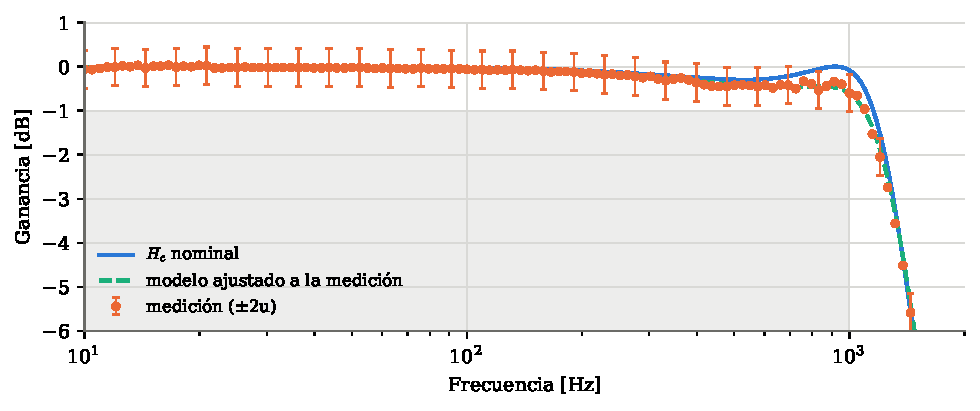
\includegraphics[width=0.92\linewidth]{fig_mediciones_paso}
  \caption{Detalle de la banda de paso: medición, modelo nominal y modelo ajustado. La zona gris es la región prohibida de la plantilla.}
  \label{fig:mediciones_paso}
\end{figure}

\paragraph{Fase.} Hasta \qty{1}{\kilo\hertz}, la fase medida difiere del modelo ajustado en \qr{2}{\mRmsResFPaso}{\degree} rms
(\cref{fig:mediciones_fase_residuo}). Por encima, con la salida cada vez más chica, el residuo crece: es de unos pocos grados hasta el límite
del ajuste (\qr{0}{\mFMaxAjuste}{\hertz}) y llega a unos \ang{20} cerca de \qty{4.5}{\kilo\hertz}, donde la salida se acerca al piso de
medición. Es el motivo por el que el ajuste se limita a la banda de \qty{-30}{\decibel}.

\begin{figure}[H]
  \centering
  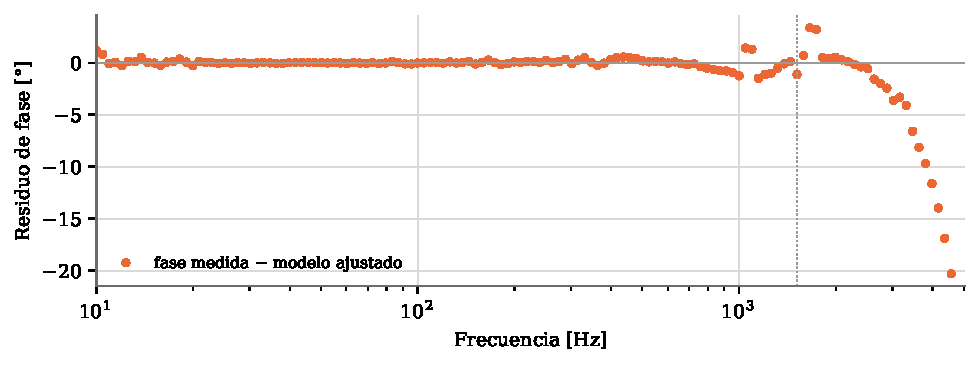
\includegraphics[width=0.9\linewidth]{fig_mediciones_fase_residuo}
  \caption{Residuo de la fase medida respecto del modelo ajustado. La línea punteada marca el paso por \ang{-180}.}
  \label{fig:mediciones_fase_residuo}
\end{figure}

\paragraph{Capacitores reales.} Invirtiendo la \cref{eq:param_circuito} con los parámetros ajustados y las resistencias medidas se estiman los
capacitores de la \cref{tab:capacitores_estimados}. Los tres capacitores llevan el código K ($\pm\qty{10}{\percent}$). $C_0$ queda prácticamente en
su valor nominal y $C_2$ \qr{1}{\mDCdos}{\percent} por encima, mientras que $C_1$ resulta \qr{1}{\mDCuno}{\percent} respecto del nominal: en el límite
de su tolerancia, con una incertidumbre de la estimación de unos \qr{0}{\mUCuno}{\percent}. Es el desvío de $C_1$ y $C_2$ en sentidos opuestos lo
que baja $Q$. Estos desvíos, junto con los de las resistencias medidas, son consistentes con el análisis de
sensibilidad: con las sensibilidades de la magnitud de la \cref{sec:sensibilidad}, predicen una variación de \qr{2}{\mDGunokPred}{\decibel} en la
ganancia a \qty{1}{\kilo\hertz}, y la medida es de \qr{2}{\mDGunokMed}{\decibel}. Como anticipaba la \cref{sec:sensibilidad}, los componentes
críticos fueron los capacitores, en este caso $C_1$ y $C_2$. Son estimaciones indirectas: heredan la incertidumbre de los parámetros ajustados,
en particular la de $f_r$, que se traslada entera a $C_0$.

\begin{table}[H]
  \centering\small
  \caption{Capacitores estimados a partir del ajuste y de las resistencias medidas. La incertidumbre combina la del ajuste y la de la medición de las
  resistencias ($\pm\qty{\mTolRMed}{\percent}$, supuesta).}
  \label{tab:capacitores_estimados}
  \tabres{tab_capacitores_estimados}
\end{table}

\paragraph{Valor del margen de diseño.} Si se aplican los mismos desvíos relativos de los componentes (capacitores estimados y resistencias medidas) a una síntesis de $H_t$ sin margen (rizado de
\qty{1}{\decibel} exacto), la atenuación máxima en la banda de paso sería de \qr{2}{\mApSinMargen}{\decibel} y el filtro \emph{no} cumpliría la
plantilla. El filtro construido, sintetizado con margen, tiene \qr{2}{\mApMaxMed}{\decibel}. La decisión de la \cref{sec:margen} se valida así con un
caso real, coherente con el Monte Carlo de esa sección: con capacitores de $\pm\qty{10}{\percent}$, como los usados (código K), el rendimiento
esperado con margen era del \qty{\vRendDiez}{\percent}, mientras que sin margen no superaba el \qty{\vRendSinMargen}{\percent} aun con capacitores de
$\pm\qty{5}{\percent}$.

\paragraph{Retardo de grupo.} Estimado a partir de la fase medida con diferencias tomadas cada 0,1~década (\cref{fig:mediciones_retardo}), el
retardo en baja frecuencia es de \qr{3}{\mTauBajaMed}{\milli\second} (nominal: \qr{3}{\mTauBajaNom}{\milli\second}) y su máximo, cerca del
borde de paso, de unos \qr{2}{\mTauMaxMed}{\milli\second} (nominal: \qr{2}{\mTauMaxNom}{\milli\second}). Por encima de
\qty{1.2}{\kilo\hertz} la estimación hereda los errores de fase del instrumento. La dispersión de los puntos en baja frecuencia es mucho menor que la
que indican las barras ($u(\varphi) = \ang{1}$ supuesta), es decir, la repetibilidad de fase del instrumento en esa zona es mejor que ese valor
conservador.

\begin{figure}[H]
  \centering
  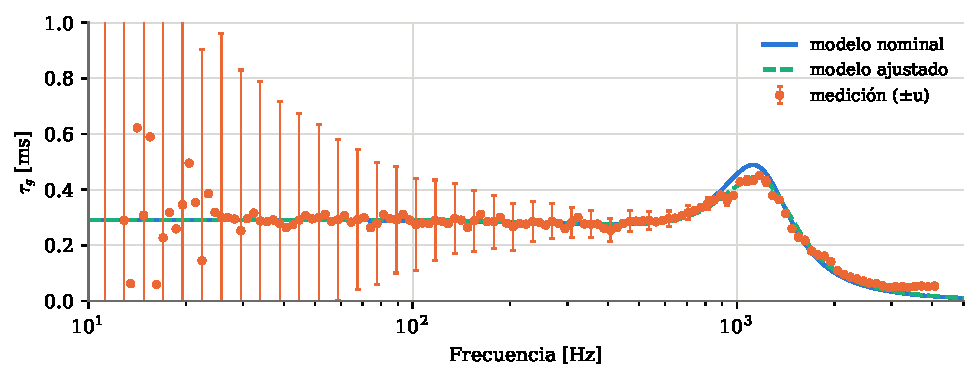
\includegraphics[width=0.9\linewidth]{fig_mediciones_retardo}
  \caption{Retardo de grupo estimado a partir de la fase medida, frente a los modelos nominal y ajustado.}
  \label{fig:mediciones_retardo}
\end{figure}

\paragraph{Respuesta al escalón.} El tiempo de subida medido, \qr{0}{\mTrMed}{\micro\second}, coincide con el del modelo ajustado con el Bode
(\qr{0}{\mTrAj}{\micro\second}) y con el nominal (\qr{0}{\mTrNom}{\micro\second}). El sobrepico medido es de
$(\nr{1}{\mSobrepicoMed} \pm \nr{1}{\mUSobrepico})\,\%$: queda entre el del modelo ajustado (\qr{1}{\mSobrepicoAj}{\percent}) y el nominal
(\qr{1}{\mSobrepicoNom}{\percent}): coincide con el primero y se aparta del segundo en menos de dos veces su incertidumbre
(\cref{fig:mediciones_escalon}). Esa incertidumbre está
dominada por la resolución vertical de la captura: \qr{1}{\mLsbmV}{\milli\volt} por nivel, el \qr{1}{2.18}{\percent} del escalón. La misma
captura incluye la salida del ecualizador del Nivel~III (\cref{sec:ec_medicion}).

\begin{figure}[H]
  \centering
  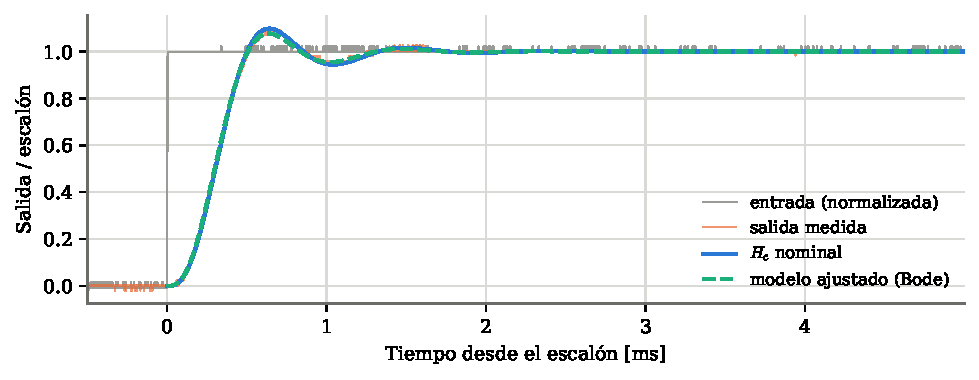
\includegraphics[width=0.9\linewidth]{fig_mediciones_escalon}
  \caption{Respuesta al escalón de \qty{2}{\volt} medida, frente a los modelos nominal y ajustado.}
  \label{fig:mediciones_escalon}
\end{figure}

\paragraph{Gran señal.} El ensayo de recorte no pudo realizarse. A \qty{936}{\hertz} la ganancia es prácticamente unitaria y, según la simulación,
la salida recorta en $\pm\qty{\vGSmaxOnce}{\volt}$; hace falta entonces una entrada de más de unos \qty{10.5}{\volt} de pico, y el generador entrega
como máximo \qty{20}{\volt} pico a pico (\qty{10}{\volt} de pico). Con esa amplitud la salida esperada es de unos \qty{10}{\volt} de pico, apenas por
debajo del recorte: el filtro no satura con ninguna señal que el generador pueda entregar, aunque el margen es chico (con $\pm\qty{\mVcc}{\volt}$ el
límite real puede quedar unas décimas de volt por debajo del simulado). El ensayo podría completarse con un amplificador previo o bajando la
alimentación, por ejemplo a $\pm\qty{9}{\volt}$, donde el recorte se espera cerca de $\pm\qty{7.5}{\volt}$.

}{%
\pendiente{cargar las mediciones en \texttt{mediciones/} y ejecutar el notebook~04.}
}

\section{Nivel II: análisis estadístico de tolerancias}
\label{sec:nivel2}

Este nivel optativo estudia cómo se dispersa la respuesta del filtro \emph{construido} (componentes de la \cref{tab:bom}, TL072) cuando los
componentes varían dentro de su tolerancia. Siguiendo la guía, se definen las distribuciones (a), se ejecutan en LTspice \nNRun{} corridas distintas por
escenario, documentando cómo se generan las muestras (b), se obtienen las distribuciones de los parámetros y el porcentaje de cumplimiento (c), se
comparan con la predicción por sensibilidad lineal de la \cref{sec:sensibilidad} (d) y se repite el análisis con tolerancias menores (e). Todo el
procesamiento está en el notebook~05.

\subsection{Distribuciones y escenarios}
Cada componente se modela como una variable aleatoria \textbf{uniforme e independiente} en $[x_0(1-t),\,x_0(1+t)]$, con $x_0$ el valor nominal y $t$
la tolerancia. Como solo se conoce el intervalo que garantiza el fabricante, es la hipótesis más conservadora. Las resistencias armadas con dos
en serie se sortean \emph{por separado}, como ocurre en el circuito real, de modo que varían nueve elementos por corrida; la resistencia del generador
($R_s = \qty{50}{\ohm}$) se mantiene fija. La \cref{tab:mc_escenarios} resume los cuatro escenarios: E1 es el ejemplo de la guía, E2 corresponde a los
componentes del prototipo (resistencias de \qty{1}{\percent} y capacitores código~K) y E3--E4 repiten el análisis con capacitores más precisos.

\begin{table}[H]
  \centering\small
  \caption{Escenarios del análisis de tolerancias.}
  \label{tab:mc_escenarios}
  \tabres{tab_mc_escenarios}
\end{table}

Un filtro \emph{cumple} si satisface la plantilla original (no la función de diseño): atenuación máxima en la banda de paso
$A_{p,\max} = \max_{f \le f_p} G - \min_{f \le f_p} G \le \qty{1}{\decibel}$ y atenuación en el borde de rechazo
$A(f_s) = \max_{f \le f_p} G - G(f_s) \ge \qty{24}{\decibel}$, con $G = 20\log_{10}|V_6/V_{in}|$. Además de estas dos magnitudes se registran la
atenuación en \qty{1}{\kilo\hertz}, la frecuencia de \qty{-3}{\decibel} y los parámetros del circuito $f_r$, $f_0$ y $Q$.

\subsection{Generación de las muestras en LTspice}
La función \texttt{mc(x,t)} de LTspice devuelve un número con distribución uniforme entre $x(1-t)$ y $x(1+t)$. Se escribe directamente en el valor
de cada elemento, por ejemplo \texttt{C1 4 6 \{mc(47n,tolC)\}}, de modo que cada elemento recibe su propio sorteo, y la directiva
\texttt{.step param run 1 500 1} repite el análisis AC \nNRun{} veces, volviendo a sortear todos los valores en cada paso. El parámetro
\texttt{run} solo numera las corridas. Las tolerancias se fijan con \texttt{.param tolR=... tolC=...}, y un netlist por escenario
(\texttt{ltspice/filtro\_TL072\_mc\_E1.cir} a \texttt{\_E4.cir}) usa el modelo de TI del TL072 con $\pm\qty{12}{\volt}$ y un barrido de
\qty{10}{\hertz} a \qty{100}{\kilo\hertz} con 50 puntos por década. El listado del escenario E2 es:

\VerbatimInput[fontsize=\footnotesize,frame=single,framesep=2mm]{\ltsdir/filtro_TL072_mc_E2.cir}

Para que el muestreo sea verificable, el netlist incluye dos \emph{sondas} desacopladas del filtro: resistencias de valor \texttt{\{mc(1,tolR)\}} y
\texttt{\{mc(1,tolC)\}} alimentadas con \qty{1}{\ampere}, cuya tensión es numéricamente el número sorteado en cada corrida y queda registrada en el
\texttt{.log}. Como en la \cref{sec:ltspice}, antes de correr LTspice el netlist se resolvió con el solver nodal propio, con cada \texttt{mc()}
reemplazado por su valor central y AO ideales: coincide con la transferencia del circuito con un error relativo máximo de \num{\nErrNet}.

\subsubsection{Verificación del muestreo}
Las cuatro corridas de LTspice (versión 24.1.10) completaron los \nNRun{} pasos de cada escenario y \num{\nVerifDistintasMin} de cada \num{\nNRun}
resultados de $A(\qty{1}{\kilo\hertz})$ son distintos entre sí: \textbf{las corridas son efectivamente distintas}. Los números sorteados por las sondas
cubren el intervalo declarado y su distribución es compatible con la uniforme (prueba de Kolmogorov--Smirnov, $p \ge \num{\nKSsondaMin}$;
\cref{fig:mc_muestreo}).

\begin{figure}[H]
  \centering
  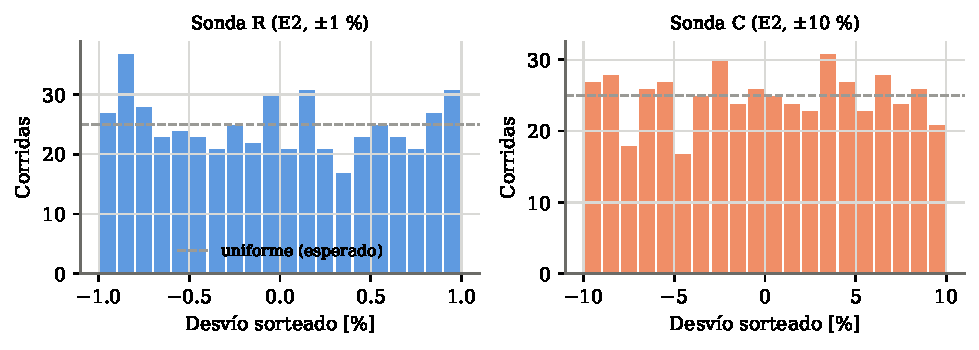
\includegraphics[width=0.85\textwidth]{fig_mc_muestreo}
  \caption{Números sorteados por las sondas en las \nNRun{} corridas del escenario E2, expresados como desvío respecto del nominal. La línea
  punteada es la altura esperada para una distribución uniforme.}
  \label{fig:mc_muestreo}
\end{figure}

Las sondas mostraron además que \textbf{LTspice usa siempre la misma secuencia de números aleatorios}: en los cuatro escenarios, y en ejecuciones
distintas, los desvíos normalizados $u = (x/x_0 - 1)/t$ son idénticos. Cada escenario es una muestra válida, pero los cuatro comparten los mismos
sorteos, escalados por su tolerancia; en estadística esto se conoce como \emph{números aleatorios comunes} y tiene una ventaja: las diferencias entre
escenarios se deben solo a las tolerancias y no al azar del muestreo. La contrapartida es que cualquier particularidad de la muestra aparece en los
cuatro escenarios a la vez.

Para examinar el generador se armó el netlist \texttt{filtro\_mc\_sondas.cir}: los mismos nueve elementos, con los mismos nombres y en el mismo orden
que el del escenario E2, pero aislados del filtro y excitados de modo que su valor quede registrado (las resistencias con \qty{1}{\ampere}, los
capacitores con \qty{1}{\volt} a \qty{1}{\kilo\hertz}). Sus sondas coinciden exactamente con las del Monte Carlo E2, de modo que este netlist
\textbf{recupera el valor de los nueve componentes en cada una de las \nNRun{} corridas}. Con esos valores se verificó lo siguiente.
\begin{itemize}
  \item \textbf{Contraste corrida por corrida} (\cref{fig:mc_por_corrida}): con los mismos componentes, la transferencia exacta con AO ideales y
        LTspice con el TL072 difieren como máximo en \qty{\nPcMaxAp}{\decibel} en $A_{p,\max}$ y \qty{\nPcMaxGunok}{\decibel} en
        $A(\qty{1}{\kilo\hertz})$. En $f_0$ y $Q$ las diferencias son prácticamente constantes, de \qty{\nPcMedFo}{\percent} y
        \qty{\nPcMedQ}{\percent}: es el efecto del GBW finito del TL072 previsto en la \cref{sec:sensibilidad}. En $f_{-3\,\text{dB}}$ la diferencia
        media es de \qty{\nPcMedFtres}{\percent}, a la que también contribuye la interpolación de \texttt{.meas} sobre la grilla de 50 puntos por
        década. Solo \nPcVeredictos{} de los \num{2000} circuitos simulados recibe un veredicto de cumplimiento distinto, un caso de E1 que está
        justo en el límite de \qty{1}{\decibel}.
  \item \textbf{Distribución y correlaciones de los sorteos}: los once sorteos de cada corrida son compatibles con la distribución uniforme. Entre los
        55 pares posibles, \nParesFuera{} superan el límite del \qty{95}{\percent} para variables independientes ($|r| < \num{\nRLimite}$), lo
        esperable por azar (unos 3). Pero el par $C_1$--$C_2$ tiene una correlación muestral de $r = \num{\nRCunoCdos}$, poco probable por azar.
        Como $\ln f_0 \propto -(\ln C_1 + \ln C_2)/2$ y $\ln Q \propto (\ln C_1 - \ln C_2)/2$, esa correlación agranda la dispersión de $f_0$ y
        achica la de $Q$, y explica por qué en esta muestra $\sigma(f_0)$ resulta un \qty{10}{\percent} mayor y $\sigma(Q)$ un \qty{7}{\percent}
        menor que lo esperado (\cref{tab:mc_dispersion}).
  \item \textbf{Secuencia larga}: para decidir si esa correlación es un defecto del generador o una particularidad de la muestra se corrió el mismo
        netlist con \num{5000} pasos (\texttt{filtro\_mc\_sondas\_5000.cir}). Sus primeras 500 corridas son idénticas a las anteriores. En las
        \num{5000}, la correlación $C_1$--$C_2$ es $r = \num{\nRCunoCdosLargo}$, dentro del límite de $\pm\num{\nRLimiteLargo}$, y solo
        \nParesFueraLargo{} de los 55 pares lo superan. En los nueve bloques de 500 corridas que siguen al primero, $r(C_1, C_2)$ varía entre
        \num{\nRBloqMin} y \num{\nRBloqMax}. La correlación de \num{\nRBloqUno} es entonces una \textbf{particularidad de las primeras 500 corridas
        de la secuencia fija de LTspice}, no un defecto del generador.
\end{itemize}
En consecuencia, las 500 corridas de LTspice son una muestra legítima pero particular. Para estimar la población se usa la referencia de Python
con \num{\nMPy} muestras, y la comparación con LTspice se hace teniendo en cuenta su error muestral.

\begin{figure}[H]
  \centering
  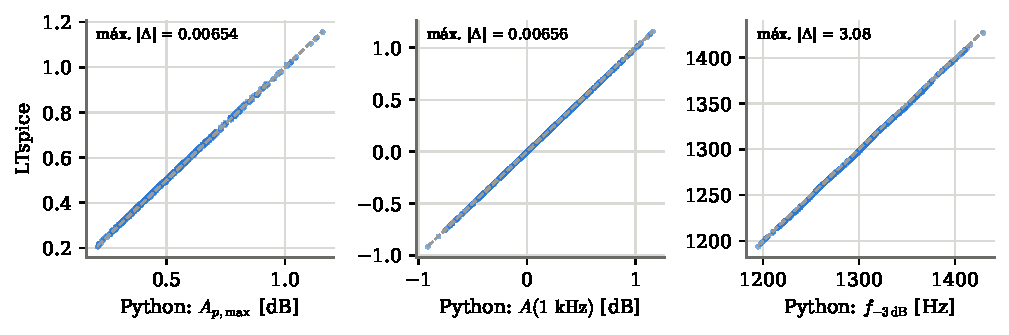
\includegraphics[width=\textwidth]{fig_mc_por_corrida}
  \caption{Contraste corrida por corrida del escenario E2: cada punto es un circuito del Monte Carlo, evaluado en LTspice (TL072) y en Python
  (transferencia exacta, AO ideales) con los mismos valores de componentes, recuperados con \texttt{filtro\_mc\_sondas.cir}.}
  \label{fig:mc_por_corrida}
\end{figure}

\subsection{Referencia en Python y predicción lineal}
Como referencia independiente de LTspice, el mismo experimento se repite en Python con \num{\nMPy} muestras por escenario, sobre la transferencia
exacta del circuito con AO ideales, en la misma grilla de frecuencias que LTspice y con las mismas definiciones de $A_{p,\max}$ y $A(f_s)$.

La predicción lineal usa las sensibilidades de la \cref{sec:sensibilidad}, ahora respecto de los nueve elementos. Una variación relativa
$\delta_x$ de cada elemento produce $\Delta P \approx \sum_x S^P_x\,\delta_x$ y, para variables uniformes independientes
($\sigma_{\delta_x} = t_x/\sqrt{3}$),
\begin{equation}
  \sigma_P \approx \sqrt{\sum_x \left(S^P_x\right)^2 \frac{t_x^2}{3}} .
  \label{eq:sigma_lineal}
\end{equation}
$A_{p,\max}$ es el máximo de la atenuación sobre la banda de paso y no es una función lineal de los componentes. En el filtro nominal ese máximo está
en el valle interior del rizado, cerca de \qty{530}{\hertz}, pero cuando $f_0$ o $f_r$ bajan pasa al borde de \qty{1}{\kilo\hertz}. Por eso, para
predecir su distribución se usa un \emph{Monte Carlo linealizado}: con las mismas muestras, la ganancia en cada frecuencia de la grilla se aproxima por
$G_0(f) + \sum_x S^{G}_x(f)\,\delta_x$ y luego se aplican las mismas definiciones. Así la no linealidad del máximo se conserva, pero cada ganancia se
evalúa con la aproximación de primer orden.

\subsection{Resultados}
La \cref{fig:mc_curvas} muestra las \nNRun{} respuestas del escenario E2, junto con la nominal y el prototipo medido; la
\cref{fig:mc_histogramas} muestra las distribuciones de los parámetros y la \cref{fig:mc_rendimiento} y la \cref{tab:mc_rendimiento} resumen el
porcentaje de cumplimiento.

\begin{figure}[H]
  \centering
  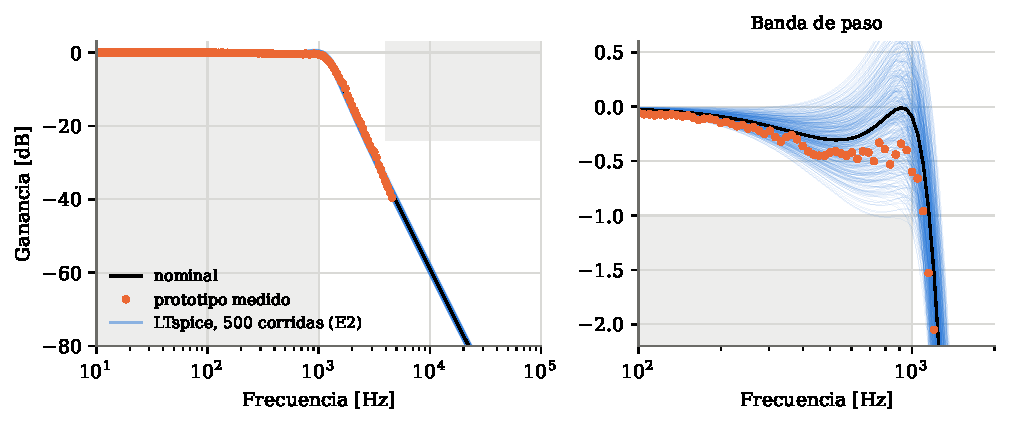
\includegraphics[width=\textwidth]{fig_mc_curvas}
  \caption{Las \nNRun{} respuestas del escenario E2 (LTspice, TL072), la respuesta nominal y el prototipo medido (\cref{sec:mediciones}). Las
  zonas grises son las regiones prohibidas por la plantilla. A la derecha, detalle de la banda de paso.}
  \label{fig:mc_curvas}
\end{figure}

\begin{figure}[H]
  \centering
  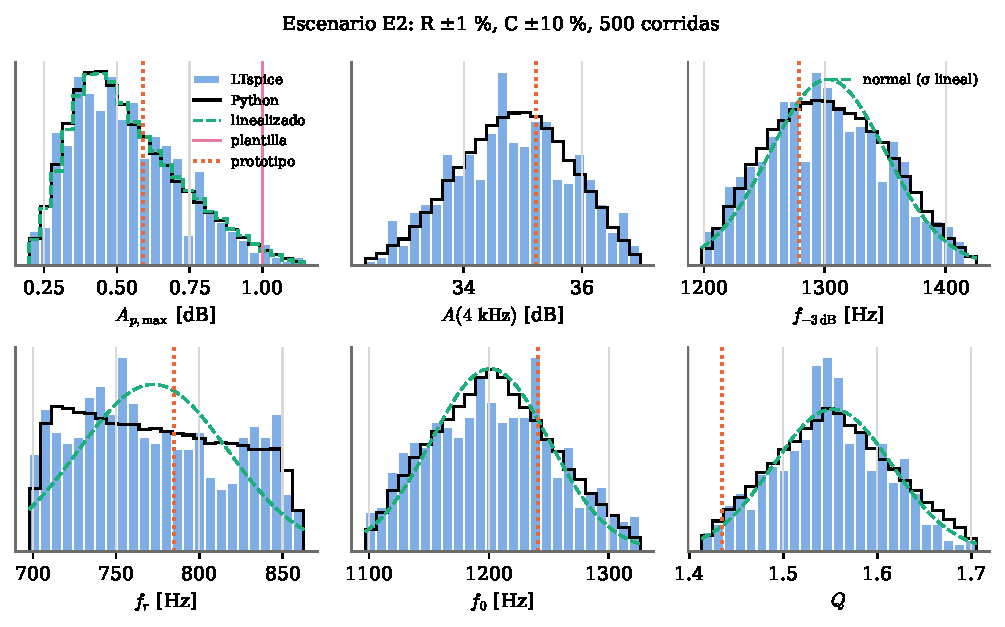
\includegraphics[width=\textwidth]{fig_mc_histogramas}
  \caption{Distribuciones del escenario E2: LTspice (\nNRun{} corridas, barras), Python (\num{\nMPy} muestras, escalones) y predicción lineal (para
  $A_{p,\max}$, el Monte Carlo linealizado; para $f_{-3\,\text{dB}}$, $f_r$, $f_0$ y $Q$, una normal con la $\sigma$ de la
  \cref{eq:sigma_lineal}). La línea vertical continua es el límite de la plantilla y la punteada, el prototipo medido.}
  \label{fig:mc_histogramas}
\end{figure}

\begin{figure}[H]
  \centering
  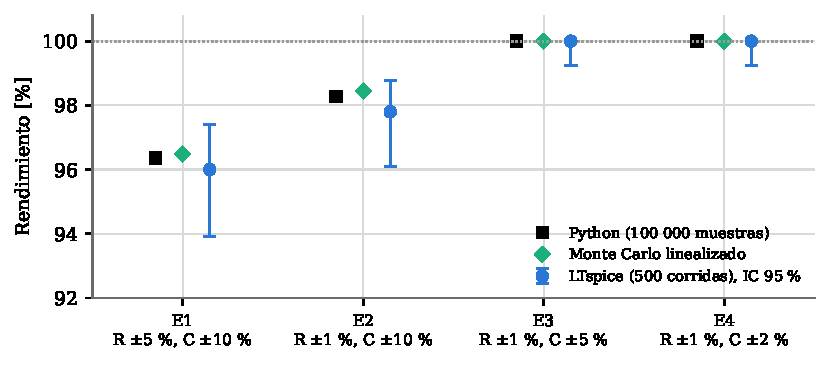
\includegraphics[width=0.85\textwidth]{fig_mc_rendimiento}
  \caption{Porcentaje de filtros que cumplen la plantilla en cada escenario. Las barras de LTspice son el intervalo de confianza del
  \qty{95}{\percent} (Wilson) para \nNRun{} corridas.}
  \label{fig:mc_rendimiento}
\end{figure}

\begin{table}[H]
  \centering\small
  \caption{Rendimiento (porcentaje de filtros que cumplen la plantilla) y percentil 95 de $A_{p,\max}$.}
  \label{tab:mc_rendimiento}
  \tabres{tab_mc_rendimiento}
\end{table}

\paragraph{Cumplimiento.} Con los componentes del prototipo (E2), LTspice da un rendimiento del \qty{\nRendLtDos}{\percent} (intervalo del
\qty{95}{\percent}: \numrange{\nRendLtInfDos}{\nRendLtSupDos}), compatible con el \qty{\nRendPyDos}{\percent} de Python y con el
\qty{\vRendDiez}{\percent} estimado en la etapa de diseño (\cref{sec:margen}). En E1 (resistencias de \qty{5}{\percent}) baja al \qty{\nRendLtUno}{\percent}.
En todos los casos la condición que falla es la del rizado: la atenuación a \qty{4}{\kilo\hertz} nunca baja de \qty{\nAcuatroMinLtUno}{\decibel},
contra \qty{24}{\decibel} exigidos, y la atenuación mínima entre \qty{4}{\kilo\hertz} y \qty{100}{\kilo\hertz} coincide en cada corrida con la de
\qty{4}{\kilo\hertz}: el TL072 no deja pasar señal en alta frecuencia en ninguna corrida. Sin el margen de diseño de la \cref{sec:margen}, el
rendimiento sería de apenas un \qty{\vRendSinMargen}{\percent}, aun con capacitores de \qty{\pm 5}{\percent}.

\paragraph{Distribuciones.} $A_{p,\max}$ tiene una distribución asimétrica, con cola hacia valores altos: es el máximo de la atenuación sobre la
banda de paso y, cuando $f_0$ o $f_r$ bajan, el máximo salta del valle interior del rizado al borde de \qty{1}{\kilo\hertz}. $f_r$ depende casi solo
de $C_0$ (\qty{\pm 10}{\percent}) y de $R_0$ (\qty{\pm 1}{\percent}), por lo que su distribución es prácticamente uniforme. $f_0$ y $Q$ combinan
dos capacitores y tienen una forma triangular; $A(\qty{4}{\kilo\hertz})$ y $f_{-3\,\text{dB}}$ combinan más elementos y se acercan a una normal.
En los cuatro escenarios, la prueba de Kolmogorov--Smirnov entre LTspice y Python no rechaza la igualdad de distribuciones para $A_{p,\max}$ ni para
$A(\qty{1}{\kilo\hertz})$ ($p \ge \num{0.4}$). Solo en E4, donde la dispersión es más chica, rechaza para $f_{-3\,\text{dB}}$ ($p = \num{0.001}$) y, en el límite, para $Q$
($p = \num{0.04}$): los corrimientos sistemáticos del modelo con TL072 medidos en el contraste corrida por corrida
(\qty{\nPcMedFtres}{\percent} y \qty{\nPcMedQ}{\percent}) ya no son despreciables frente a una dispersión de menos del \qty{1}{\percent}.

\paragraph{Comparación con la sensibilidad lineal (d).} La \cref{tab:mc_dispersion} compara las desviaciones estándar del escenario E2. La predicción
lineal coincide con el Monte Carlo de Python dentro del \qty{1}{\percent} en todos los parámetros: con tolerancias de hasta \qty{10}{\percent}, el
filtro se comporta de forma prácticamente lineal y la \cref{eq:sigma_lineal} basta para estimar la dispersión. El Monte Carlo linealizado reproduce
también el rendimiento (\qty{\nRendLinDos}{\percent} frente a \qty{\nRendPyDos}{\percent}) y el percentil 95 de $A_{p,\max}$
(\cref{tab:mc_rendimiento}). Las diferencias entre la columna de Python con \num{\nMPy} muestras y LTspice se deben a la muestra particular
analizada en la subsección anterior: evaluada en Python con los mismos 500 juegos de componentes, la dispersión coincide con la de LTspice. La
forma de la distribución, en cambio, no siempre es normal (\cref{fig:mc_histogramas}): para $f_r$, la $\sigma$ lineal es correcta, pero la
distribución es uniforme y sus colas son más cortas que las de una normal.

\begin{table}[H]
  \centering\small
  \caption{Desviación estándar de los parámetros en el escenario E2 (R $\pm\qty{1}{\percent}$, C $\pm\qty{10}{\percent}$): predicción lineal
  (\cref{eq:sigma_lineal}), Monte Carlo de Python con \num{\nMPy} muestras y con los mismos 500 juegos de componentes de LTspice, y LTspice.
  Frecuencias y $Q$ en porcentaje del valor nominal.}
  \label{tab:mc_dispersion}
  \tabres{tab_mc_dispersion_E2}
\end{table}

\paragraph{Tolerancias menores (e).} Con capacitores de \qty{\pm 5}{\percent} (E3) o \qty{\pm 2}{\percent} (E4), los 500 circuitos de LTspice y los
\num{\nMPy} de Python cumplen la plantilla. El percentil 95 de $A_{p,\max}$ baja a \qty{\nApNoventaLtTres}{\decibel} y
\qty{\nApNoventaLtCuatro}{\decibel}, respectivamente, y la dispersión de cada parámetro escala casi proporcionalmente a la tolerancia de los
capacitores, que dominan el error (la de $A(\qty{1}{\kilo\hertz})$ pasa de \qty{\nSigAunokLtDos}{\decibel} en E2 a \qty{\nSigAunokLtTres}{\decibel}
en E3 y \qty{\nSigAunokLtCuatro}{\decibel} en E4). Para un diseño de producción, pasar a capacitores código~J eliminaría prácticamente las fallas
sin cambiar la topología. Bajar la tolerancia de las resistencias, en cambio, aporta poco: de E1 a E2, con los mismos capacitores, el rendimiento
mejora apenas dos puntos.

\paragraph{El prototipo dentro de la distribución.} Con los parámetros medidos (\cref{sec:mediciones}), el prototipo es un caso
típico del escenario E2 en casi todo: un \qty{\nUbicAp}{\percent} de los circuitos simulados tiene un $A_{p,\max}$ mayor que el medido, un
\qty{\nUbicFr}{\percent} se aparta más que él en $f_r$ y un \qty{\nUbicFo}{\percent} tiene una $f_0$ más alta. El parámetro menos típico es $Q$,
\qty{7.6}{\percent} por debajo del nominal: solo un \qty{\nUbicQ}{\percent} de los circuitos simulados tiene un $Q$ más bajo. Es coherente con la
estimación de los capacitores, con $C_1$ en el límite inferior de su tolerancia y $C_2$ por encima del nominal. Aun así, el prototipo cumple la
plantilla con margen, que es justamente lo que el margen de diseño buscaba asegurar.

\paragraph{Conclusión del Nivel II.} El análisis estadístico confirma el diseño: con los componentes disponibles, cerca del \qty{98}{\percent} de los
filtros construidos cumpliría la plantilla, y la causa de las fallas restantes (el rizado, por el desvío de los capacitores) está identificada. Las
tres vías de cálculo independientes coinciden dentro del error estadístico: LTspice con el modelo del fabricante, la transferencia exacta en Python y
la predicción lineal por sensibilidades. El procedimiento quedó documentado de forma verificable: corridas distintas, distribución de los sorteos
comprobada y valores de cada corrida recuperados y contrastados uno a uno.

\section{Nivel III: ecualizador de fase pasatodo}
\label{sec:nivel3}

Un filtro Chebyshev transmite la banda de paso con poca variación de amplitud, pero no con retardo constante. Su retardo de grupo crece hacia el
borde de la banda (\cref{sec:mediciones}), de modo que las componentes de una señal cercanas a \qty{1}{\kilo\hertz} llegan más tarde que las de baja
frecuencia y la forma de onda se deforma (sobrepico y oscilación en la respuesta al escalón). Este nivel optativo diseña, simula, construye y mide un
ecualizador pasatodo que compensa esa variación \emph{en el prototipo construido}. El procesamiento está en el notebook~06.

\subsection{Banda útil y función objetivo}
\paragraph{Filtro a ecualizar.} El ecualizador se diseña para el prototipo, no para el filtro nominal, con el modelo ajustado a la medición del
filtro (\cref{sec:mediciones}: $f_r = \qr{1}{\eProtoFr}{\hertz}$, $f_0 = \qr{1}{\eProtoFo}{\hertz}$, $Q = \nr{3}{\eProtoQ}$). Su retardo de grupo, calculado
polo a polo, vale \qty{\eTauCeroF}{\milli\second} en baja frecuencia y \qty{\eTauUnokF}{\milli\second} en \qty{1}{\kilo\hertz}, con un máximo cerca
de \qty{1.15}{\kilo\hertz} (\cref{fig:ec_objetivo}). La distinción importa: el ecualizador óptimo para el prototipo, aplicado al filtro nominal, solo
reduce la variación de \qty{\eJNomSinEc}{\milli\second} a \qty{\eJNomConEcProto}{\milli\second}, porque los dos filtros difieren en unos pocos por
ciento en $f_r$ y $f_0$.

\paragraph{Banda útil.} Es la banda de paso de la plantilla, $0 < f \le f_p = \qty{1}{\kilo\hertz}$: la que el filtro transmite y en la que importa
la forma de onda. Por encima de $f_p$ la señal está atenuada y su retardo no tiene consecuencias.

\paragraph{Función objetivo.} Un retardo constante solo desplaza la señal en el tiempo; lo que la deforma es la \emph{variación} del retardo. Se
minimiza entonces la variación pico a pico del retardo total en la banda útil (criterio \emph{minimax}),
\begin{equation}
  J = \max_{0 < f \le f_p} \tau_\text{tot}(f) - \min_{0 < f \le f_p} \tau_\text{tot}(f), \qquad \tau_\text{tot} = \tau_\text{filtro} + \tau_\text{ec},
  \label{eq:J_ecualizador}
\end{equation}
y como medida complementaria se informa el valor eficaz de la desviación respecto de la media, $J_\text{rms}$. Sin ecualizar,
$J = \qr{3}{\eJsinEc}{\milli\second}$ (\qty{50}{\percent} del retardo en continua). El precio de ecualizar es un retardo total mayor, que para la mayoría
de las aplicaciones (audio, instrumentación) no tiene consecuencias.

\begin{figure}[H]
  \centering
  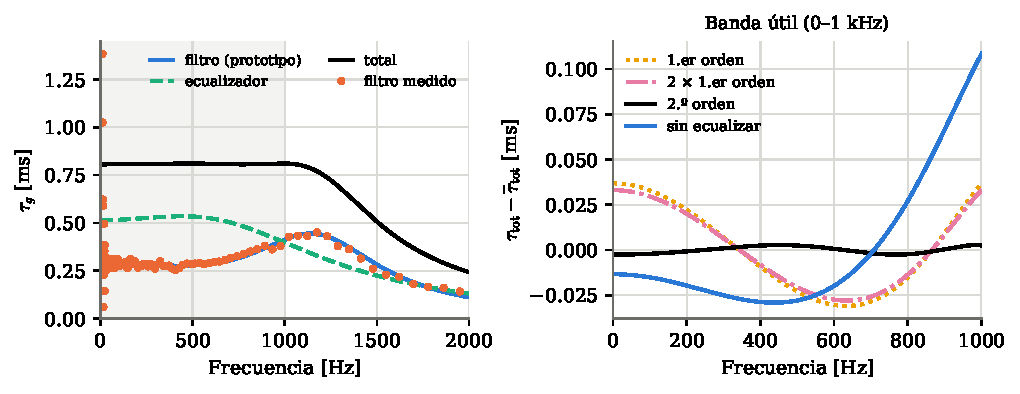
\includegraphics[width=\textwidth]{fig_ec_objetivo}
  \caption{Izquierda: retardo de grupo del prototipo (modelo ajustado y medición), del ecualizador de 2.º orden óptimo y de la cascada. Derecha:
  desviación del retardo total respecto de su media en la banda útil, para las alternativas de la \cref{tab:ec_orden}.}
  \label{fig:ec_objetivo}
\end{figure}

\subsection{Orden del ecualizador}
Para aplanar $\tau_\text{tot}$, el ecualizador debe aportar mucho retardo en baja frecuencia y poco cerca de $f_p$. Se compararon cuatro
alternativas, optimizando $J$ en cada caso (\cref{tab:ec_orden}). Los pasatodos de 1.er orden, cuyo retardo $2\omega_a/(\omega_a^2+\omega^2)$
decrece demasiado despacio, apenas reducen $J$ a la mitad, incluso con dos secciones. El pasatodo de 2.º orden
\begin{equation}
  H_\text{ec}(s) = k\,\frac{s^2 - (\omega_0/Q)\,s + \omega_0^2}{s^2 + (\omega_0/Q)\,s + \omega_0^2}
\end{equation}
tiene un retardo casi plano hasta unos \qty{600}{\hertz} que cae justo donde sube el del filtro: con $f_0 = \qty{\eFoAP}{\hertz}$ y
$Q = \num{\eQAP}$ reduce $J$ a \qty{\eJOpt}{\milli\second}, \num{\eMejoraOpt} veces menos, con un solo AO. Agregarle una sección de 1.er orden
mejora el óptimo teórico (\qty{\eJDosMasUno}{\milli\second}), pero esa mejora no es alcanzable: como se muestra más adelante, con componentes reales
$J$ queda limitado por la dispersión de $f_0$ y $Q$ del ecualizador mucho antes de llegar al óptimo de un solo AO. Se elige entonces el pasatodo
de 2.º orden con un AO.

\begin{table}[H]
  \centering\small
  \caption{Alternativas de ecualizador para el prototipo, con sus parámetros óptimos. La mejora es el cociente entre $J$ sin ecualizar y $J$ con el
  ecualizador; $\tau_\text{tot}(0)$ es el retardo total en continua.}
  \label{tab:ec_orden}
  \tabres{tab_ec_orden}
\end{table}

\subsection{Topología y derivación}
Se usa una celda de un solo AO (\cref{fig:ec_esquema}): un pasabanda de realimentación múltiple (Delyiannis--Friend) que recibe la entrada a través
de $R_1$ y una fracción $k = R_b/(R_a+R_b)$ de la misma entrada en la entrada no inversora. El análisis nodal con AO ideal ($V_- = V_+ = kV_e$),
hecho con SymPy antes de imponer valores, da
\begin{equation}
  H_\text{ec}(s) = \frac{k\left[s^2 + b_1 s + \omega_0^2\right]}{s^2 + \dfrac{C_1+C_2}{R_2C_1C_2}\,s + \dfrac{1}{R_1R_2C_1C_2}}, \qquad
  b_1 = \frac{k(C_1R_1 + C_1R_2 + C_2R_1) - C_1R_2}{k\,C_1C_2R_1R_2},
\end{equation}
con $\omega_0 = 1/\sqrt{R_1R_2C_1C_2}$ y $Q = \sqrt{R_2/R_1}\,\sqrt{C_1C_2}/(C_1+C_2)$.

\begin{figure}[H]
  \centering
  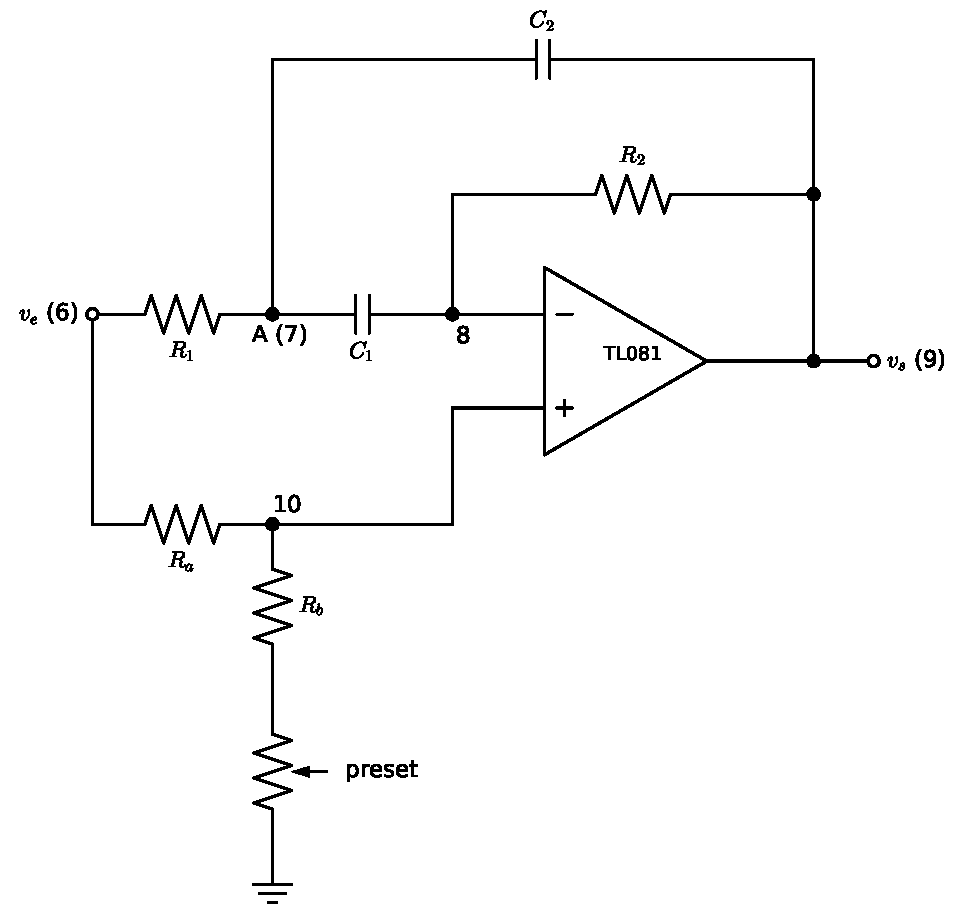
\includegraphics[width=0.62\textwidth]{fig_ec_esquema}
  \caption{Ecualizador pasatodo de 2.º orden con un AO (TL081). El preset multivuelta, conectado como resistencia variable, ajusta $k$.}
  \label{fig:ec_esquema}
\end{figure}

El término independiente del numerador coincide \emph{siempre} con el del denominador: ceros y polos tienen el mismo módulo para cualquier valor de los
componentes. La condición de pasatodo se reduce entonces a una sola ecuación, $b_1 = -\omega_0/Q$, que fija
\begin{equation}
  \frac{1}{k} - 1 = \frac{2R_1(C_1+C_2)}{R_2C_1} \;\overset{C_1 = nC_2}{=}\; \frac{2}{Q^2(1+n)} .
  \label{eq:k_pasatodo}
\end{equation}
La ganancia del ecualizador es $k < 1$ en todas las frecuencias. Conviene $n$ grande para que $k$ se acerque a~1: con $n = 1$ sería
$k = Q^2/(1+Q^2) \approx 0{,}29$. Las sensibilidades son las del pasabanda de realimentación múltiple, $S^{\omega_0}_x = -1/2$ para los cuatro
elementos, $S^{Q}_{R_1} = -S^{Q}_{R_2} = -1/2$ y $S^Q_{C_1} = -S^Q_{C_2} = (C_2 - C_1)/[2(C_1+C_2)] = -\num{\eSQC}$ para $n \approx 10$.

\paragraph{Error de magnitud y ajuste.} Si la condición se cumple solo aproximadamente, $b_1 = -(1-\varepsilon)\,\omega_0/Q$, la magnitud vale $k$ en
continua y en alta frecuencia y $k(1-\varepsilon)$ en $f_0$: aparece una campana centrada en $f_0$. La cancelación es muy sensible:
$\partial\varepsilon/\partial(\ln k) = C_1R_2/[R_1k(C_1+C_2)] = \num{\eSEpsK}$, de modo que un error de \qty{1}{\percent} en $k$ produce
\qty{\eDbPorPctK}{\decibel} de error de magnitud en $f_0$, y con resistencias fijas de \qty{1}{\percent} la magnitud no quedaría plana. Pero $k$ no
aparece en el denominador: ajustar $k$ con un preset \textbf{corrige el error de magnitud sin mover $f_0$ ni $Q$}, por lo que el circuito tiene un
ajuste natural e independiente.

\subsection{Componentes}
Todas las combinaciones de capacitores disponibles con $n \ge 1$ tienen la misma robustez en $J$, porque la limita la tolerancia de los
capacitores, que mueve $f_0$. Se eligió $C_1 = \qty{47}{\nano\farad}$ y $C_2 = \qty{4.7}{\nano\farad}$ ($n = 10$), que dan $k = \num{\eKAP}$
(\qty{\eKAPdB}{\decibel}) y resistencias de algunos kilohms a decenas de kilohms, y son los mismos valores que ya usa el filtro. Antes de calcular
las resistencias se midieron los dos capacitores con el UT61D+ (exactitud de ±(3\,\% + 5 dígitos), unos ±\qty{\eTolCmed}{\percent}), y $R_1$ y $R_2$
se calcularon con esos valores (\cref{tab:ec_componentes}, columna ``Cálculo''). El divisor de $k$ usa $R_a = \qty{10}{\kilo\ohm}$ y $R_b$
formada por una resistencia fija más un preset multivuelta de \qty{10}{\kilo\ohm}, conectado como resistencia variable.

El montaje inicial se armó antes de la medición definitiva del filtro, con resistencias calculadas a partir de una estimación preliminar de sus
parámetros: $R_1 = \qty{\eRunoI}{\kilo\ohm}$ y $R_2 = \qty{\eRdosI}{\kilo\ohm}$ (medidas), frente a \qty{\eRunoE}{\kilo\ohm} y \qty{\eRdosE}{\kilo\ohm}
de valores comerciales que corresponden al cálculo final. Cada resistencia se armó con dos en serie, de modo de poder sintonizar el ecualizador
cambiando solo la menor de cada par; las correcciones se describen en la \cref{sec:ec_medicion}. Con $R_b = \qty{19.92}{\kilo\ohm}$ fija más el preset,
$k$ se ajusta entre \num{\eKMinM} y \num{\eKMaxM}; con el montaje final, la magnitud plana ($k = \num{\eKM}$) se obtiene con el preset en unos
\qty{\eRPresetM}{\kilo\ohm}.

\begin{table}[H]
  \centering\small
  \caption{Componentes del ecualizador: valores de cálculo (con los capacitores medidos), montaje inicial y montaje final tras la
  sintonía (\cref{sec:ec_medicion}). Las resistencias del montaje son valores medidos con el UT61D+.}
  \label{tab:ec_componentes}
  \tabres{tab_ec_componentes}
\end{table}

\subsection{Robustez}
La \cref{fig:ec_robustez} muestra la distribución de $J$ obtenida por Monte Carlo (\num{4000} muestras, resistencias de \qty{\pm 1}{\percent},
incertidumbre del ajuste del prototipo incluida) para cuatro estrategias de montaje. Con capacitores nominales de \qty{\pm 10}{\percent} la mejora
mediana sería de apenas \num{\eMejoraCincuentaNom} veces (\num{\eMejoraNoventaNom} en el \qty{90}{\percent} de los casos). Medir los
capacitores la lleva a \num{\eMejoraCincuentaMed}, y ajustar además $k$ con el preset a \num{\eMejoraCincuentaAj}
(\num{\eMejoraNoventaAj} en el \qty{90}{\percent} de los casos). Si después de medir el ecualizador armado se corrigieran $R_1$ y $R_2$ con los
valores de $f_0$ y $Q$ ajustados a su fase, la mejora mediana llegaría a \num{\eMejoraCincuentaCorr}. El montaje usó la tercera estrategia y, después de medir, también la
cuarta (\cref{sec:ec_medicion}).

\begin{figure}[H]
  \centering
  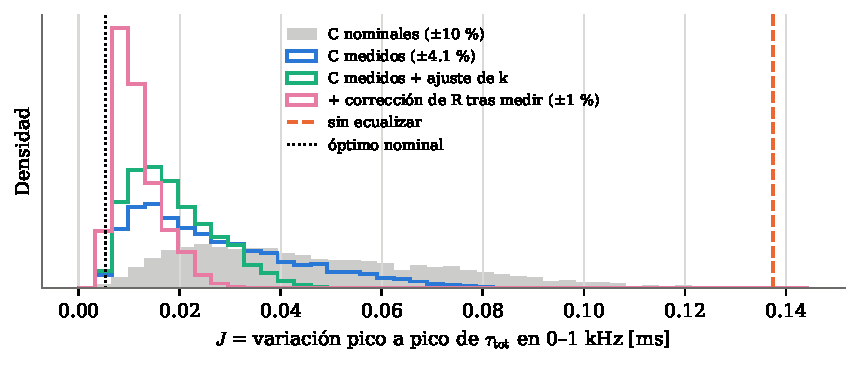
\includegraphics[width=0.8\textwidth]{fig_ec_robustez}
  \caption{Distribución de $J$ para el ecualizador montado sobre el prototipo, según cómo se elijan y ajusten los componentes.}
  \label{fig:ec_robustez}
\end{figure}

\subsection{Simulación}
La \cref{fig:ec_respuesta} muestra la respuesta calculada con los valores de cálculo de la \cref{tab:ec_componentes}. El retardo total queda en unos \qty{0.83}{\milli\second}
y prácticamente constante hasta \qty{1}{\kilo\hertz}; la magnitud del ecualizador es plana, de modo que la de la cascada es la del filtro
desplazada \qty{\eKAPdB}{\decibel}.

\begin{figure}[H]
  \centering
  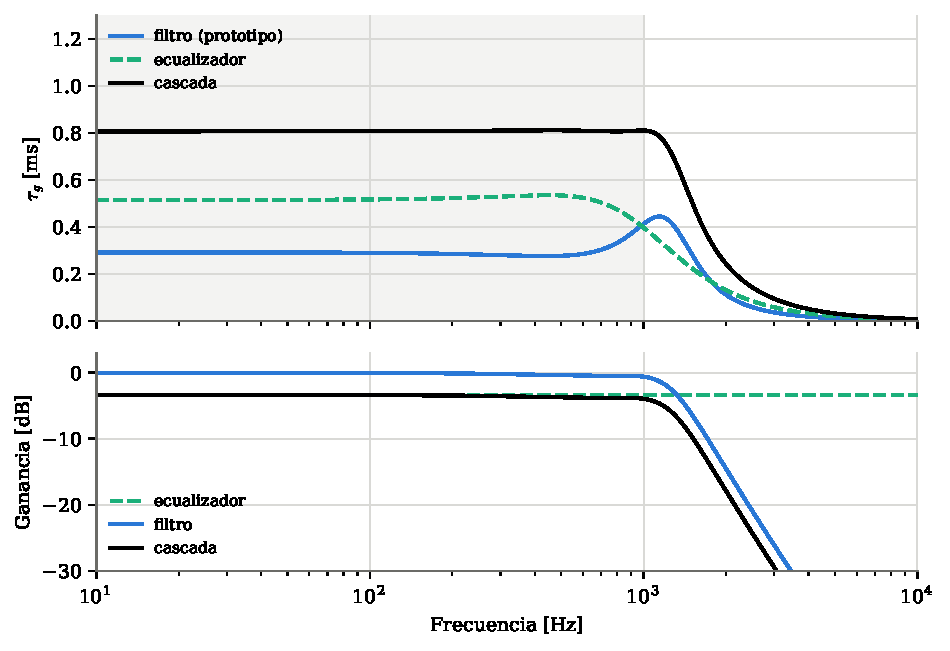
\includegraphics[width=0.85\textwidth]{fig_ec_respuesta}
  \caption{Retardo de grupo y ganancia del filtro (prototipo), del ecualizador y de la cascada, con los valores de cálculo.}
  \label{fig:ec_respuesta}
\end{figure}

Con el modelo, la respuesta al escalón cambia de forma (\cref{fig:ec_escalon_modelo}): el sobrepico baja del \qr{1}{\eSobF}{\percent} al
\qr{1}{\eSobC}{\percent} y aparece una pre-oscilación, del \qr{1}{\ePreC}{\percent}, antes de la subida. La respuesta se vuelve casi simétrica
respecto de su punto medio, que es lo característico de un sistema de fase lineal: la deformación ya no se concentra después del flanco.

\begin{figure}[H]
  \centering
  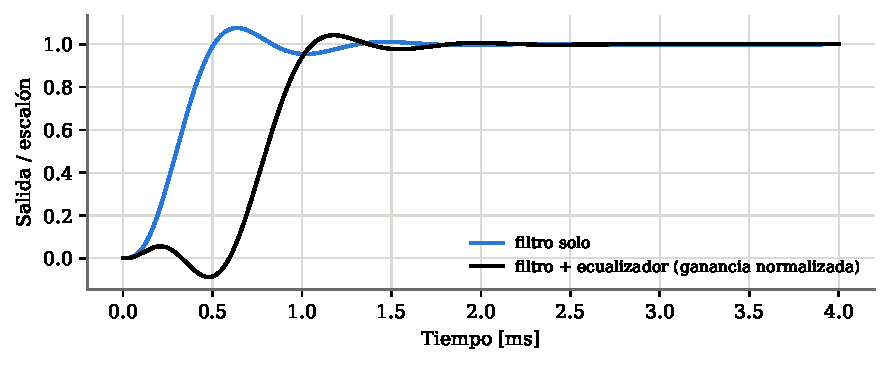
\includegraphics[width=0.8\textwidth]{fig_ec_escalon_modelo}
  \caption{Respuesta al escalón calculada del filtro (prototipo) y de la cascada, normalizada a ganancia unitaria.}
  \label{fig:ec_escalon_modelo}
\end{figure}

En LTspice se simularon el ecualizador solo y la cascada con el ecualizador tal como quedó montado tras la sintonía (resistencias y capacitores
medidos, preset en la posición de magnitud plana), con el macromodelo del TL072 de TI, que comparte etapa de entrada, GBW y slew rate con el TL081
del montaje. La cascada usa el filtro del prototipo reconstruido: resistencias medidas y capacitores estimados en la \cref{sec:mediciones}. Antes, el
netlist del ecualizador se verificó con el solver nodal propio, con un error relativo máximo de \num{\eErrNet} respecto de la transferencia simbólica.
\ifdefined\eLTJCascadaMs
Resultados:
\begin{itemize}
  \item la ganancia del ecualizador es de \qr{2}{\eLTEcGananciaDb}{\decibel} ($20\log k$ con $k = \num{\eKM}$) y varía menos de
        \qr{2}{\eLTEcRizadoDb}{\decibel} entre \qty{10}{\hertz} y \qty{10}{\kilo\hertz}; su retardo difiere del calculado con la transferencia ideal
        en menos de \qr{1}{\eLTEcTauErrMaxUs}{\micro\second} en la banda útil, es decir, el TL081 no introduce error apreciable a estas frecuencias;
  \item la variación del retardo en la banda útil baja de \qr{3}{\eLTJFiltroMs}{\milli\second} (filtro solo) a \qr{4}{\eLTJCascadaMs}{\milli\second}
        (cascada) (\cref{fig:ec_ltspice}). Es una mejora menor que la medida (\cref{sec:ec_medicion}), y la diferencia tiene una causa
        identificable: la simulación usa los capacitores \emph{leídos con el multímetro}, con los que el montaje final da $f_0 = \qr{1}{\eFoM}{\hertz}$
        y $Q = \nr{3}{\eQM}$, un \qty{3.4}{\percent} por encima del objetivo en $Q$. La sintonía, en cambio, se hizo sobre la respuesta medida, es
        decir, sobre los capacitores reales. Los capacitores que explican el $f_0$ y el $Q$ medidos con las resistencias montadas son
        \qty{49.5}{\nano\farad} y \qty{4.63}{\nano\farad}, a $+\qty{4.5}{\percent}$ y $-\qty{3.2}{\percent}$ de las lecturas, del orden de la
        exactitud del UT61D+. La simulación confirma así lo que mostró el análisis de robustez: con capacitores conocidos al
        \qty{4}{\percent}, el ecualizador solo alcanza el óptimo si se sintoniza midiendo;
  \item la respuesta al escalón (\cref{fig:ec_ltspice_escalon}) tiene la forma del modelo: el sobrepico baja del \qr{1}{\eLTEscSobFPct}{\percent} al
        \qr{1}{\eLTEscSobEPct}{\percent} y aparece una pre-oscilación del \qr{1}{\eLTEscPreEPct}{\percent} antes de la subida.
\end{itemize}

\begin{figure}[H]
  \centering
  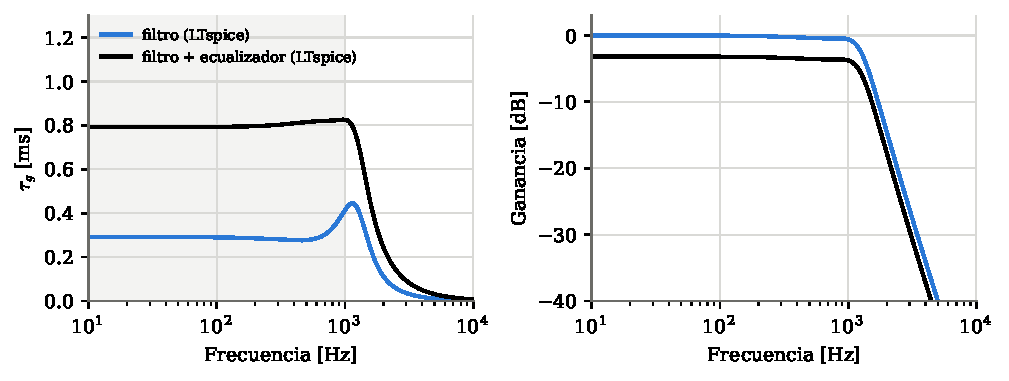
\includegraphics[width=\textwidth]{fig_ec_ltspice}
  \caption{LTspice: retardo de grupo y ganancia del filtro del prototipo solo y con el ecualizador.}
  \label{fig:ec_ltspice}
\end{figure}

\begin{figure}[H]
  \centering
  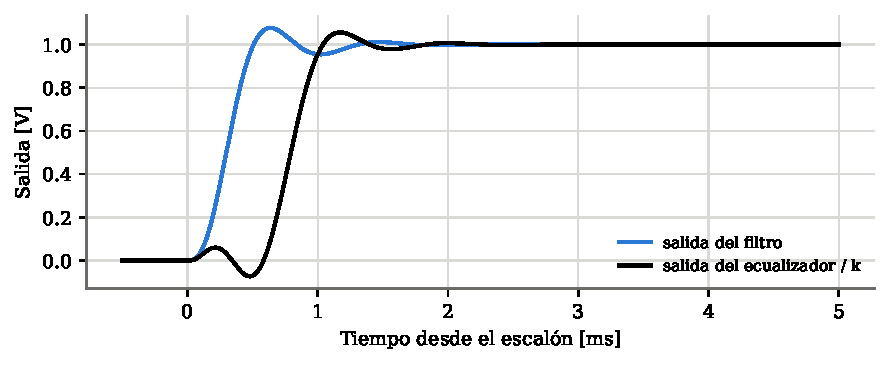
\includegraphics[width=0.8\textwidth]{fig_ec_ltspice_escalon}
  \caption{LTspice: respuesta al escalón de \qty{1}{\volt} a la salida del filtro y a la salida del ecualizador (dividida por $k$).}
  \label{fig:ec_ltspice_escalon}
\end{figure}
\else
\pendiente{correr en LTspice los tres netlists del ecualizador (montaje final) y volver a ejecutar el notebook~06.}
\fi

\subsection{Implementación y medición}
\label{sec:ec_medicion}
El ecualizador se arma con un TL081 a la salida del filtro, con \qty{\pm 12}{\volt} y desacople de \qty{100}{\nano\farad}. El procedimiento
(\texttt{mediciones/nivel3/README.md}) tiene cinco pasos:
\begin{enumerate}
  \item medir los capacitores y las resistencias;
  \item ajustar el preset con el ecualizador solo, hasta que la amplitud de salida a \qty{940}{\hertz} iguale la de \qty{20}{\hertz} (si a
        \qty{940}{\hertz} es menor, $k$ es demasiado grande);
  \item medir con el modo Bode el ecualizador solo y ajustar su modelo ($f_0$, $Q$, $k$, $\varepsilon$) a la ganancia y la fase medidas;
  \item opcionalmente, corregir $R_1$ y $R_2$ si $f_0$ o $Q$ se apartan más de \qty{2}{\percent};
  \item medir la cascada con el modo Bode, con los mismos ajustes que la medición del filtro solo.
\end{enumerate}

Con el Bode del Rigol, el retardo obtenido por diferencias de fase entre puntos vecinos es demasiado ruidoso para resolver variaciones de
\qty{0.01}{\milli\second}. Por eso la mejora se cuantifica de dos maneras independientes: (i) $J$ calculado con el modelo de la cascada ajustado a su
Bode, con su incertidumbre propagada, y (ii) una métrica sin modelo, el desvío de la fase medida respecto de la recta que mejor la aproxima entre
\qty{20}{\hertz} y \qty{1}{\kilo\hertz}. Una fase lineal equivale a un retardo constante, de modo que ese desvío mide directamente la distorsión de
fase. Según el modelo, el desvío máximo pasa de unos \ang{5.6} en el filtro solo a \ang{0.1} con el ecualizador óptimo.

\paragraph{Sintonía.} El ecualizador solo se midió tres veces; entre una medición y la siguiente se cambió la resistencia menor de cada par
(\cref{tab:ec_sintonia}). En cada medición se ajustaron $f_0$, $Q$, $k$ y $\varepsilon$ a la ganancia y la fase, y se calculó el $J$ que daría
el ecualizador sobre el filtro medido.
\begin{itemize}
  \item \textbf{Montaje inicial.} $f_0$ quedó un \qty{4.5}{\percent} por debajo del objetivo. La calibración de canales descartó que el error fuera
        del instrumento. A partir de $f_0$ y $Q$ medidos y de las resistencias montadas se calcularon los capacitores ``efectivos''
        (\qty{48.9}{\nano\farad} y \qty{4.57}{\nano\farad}, a $+\qty{3.3}{\percent}$ y $-\qty{4.4}{\percent}$ de las lecturas, del orden de la
        exactitud del UT61D+) y, con ellos, las resistencias que llevan el
        ecualizador al objetivo.
  \item \textbf{Primera corrección.} Se calculó para el objetivo que daba la estimación preliminar del filtro; por eso, respecto del objetivo final,
        no mejora $f_0$.
  \item \textbf{Segunda corrección (final).} Recalculada con la medición del filtro, deja $f_0$ a un \qty{1}{\percent} del objetivo y $Q$ a menos
        del \qty{0.5}{\percent}. La corrección se eligió con un ajuste preliminar de esa medición (\qty{982}{\hertz} y \num{0.625}); el criterio
        definitivo del notebook~04 da el objetivo de la tabla. Con aquel objetivo, un pasatodo ideal daría $J = \qty{0.0079}{\milli\second}$ en lugar
        de \qr{4}{\eJOpt}{\milli\second}: la diferencia es del orden de la incertidumbre con que se determina $J$ en la cascada
        (\qr{4}{\eMUJCas}{\milli\second}), por lo que no se hizo una tercera corrección.
\end{itemize}
El cambio de resistencias es la forma de sintonizar un circuito cuyos capacitores solo se conocen con la exactitud del multímetro. El preset, en
cambio, solo ajusta la magnitud.

\begin{table}[H]
  \centering\small
  \caption{Sintonía del ecualizador solo: resistencias medidas, $f_0$ y $Q$ ajustados a cada medición, y $J$ previsto sobre el filtro medido. La
  mejora es el cociente entre $J$ del filtro solo (\qr{4}{\eMJFil}{\milli\second}) y $J$ con el ecualizador.}
  \label{tab:ec_sintonia}
  \tabres{tab_ec_sintonia}
\end{table}

\begin{figure}[H]
  \centering
  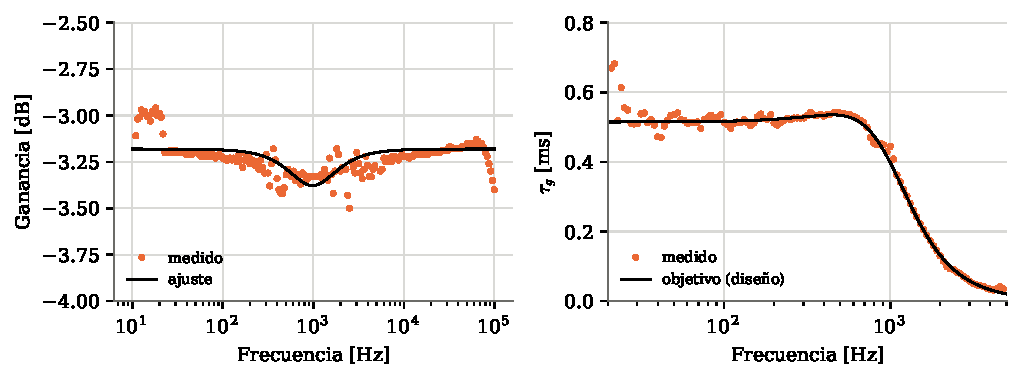
\includegraphics[width=\textwidth]{fig_ec_medicion_ap}
  \caption{Ecualizador solo, montaje final: ganancia y retardo de grupo medidos, con el modelo ajustado y el retardo del ecualizador objetivo.}
  \label{fig:ec_medicion_ap}
\end{figure}

\paragraph{Ecualizador final.} La ganancia es $k = \nr{3}{\eMApK}$ y el error de pasatodo es $\varepsilon = \nr{3}{\eMApEps} \pm \nr{3}{\eMApUEps}$,
es decir, un valle de \qr{2}{\eMApValle}{\decibel} en $f_0$. Su efecto sobre el retardo total está dentro de la incertidumbre: según qué ajuste
se use, el del ecualizador solo o el de la cascada, anularlo con el preset bajaría $J$ o lo dejaría prácticamente igual. Por eso no se retocó el
ajuste. Con ese valle, la atenuación de la cascada en \qty{1}{\kilo\hertz}, referida a su ganancia de continua, sigue por debajo de
\qty{1}{\decibel}.

\paragraph{Cascada.} La \cref{fig:ec_medicion} muestra el retardo de grupo del filtro solo y de la cascada, medidos en la misma sesión. El
retardo del filtro varía entre unos \qty{0.28}{\milli\second} y \qty{0.41}{\milli\second} en la banda de paso; el de la cascada es prácticamente
constante, de unos \qty{0.81}{\milli\second}, hasta \qty{1}{\kilo\hertz}. La consistencia de las mediciones se verificó punto a punto: la fase de la
cascada coincide con la suma de las fases del filtro y del ecualizador medidos por separado, con una diferencia mediana de
\qr{2}{\eMIncMediana}{\degree}. Solo \eMNArtef{} puntos se apartan más de \ang{2}; son errores del instrumento cerca del paso por \ang{-180} y se
excluyen de la métrica sin modelo.

\begin{figure}[H]
  \centering
  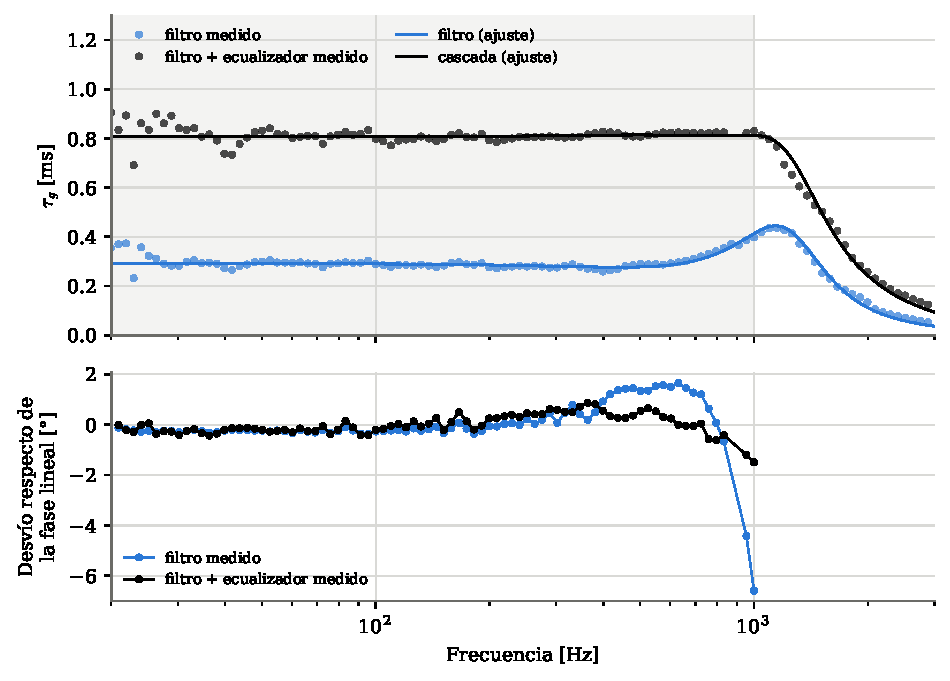
\includegraphics[width=0.95\textwidth]{fig_ec_medicion}
  \caption{Arriba: retardo de grupo medido (regresión local de la fase) del filtro solo y de la cascada, con los modelos ajustados. Abajo: desvío
  de la fase medida respecto de la recta que mejor la aproxima entre \qty{20}{\hertz} y \qty{1}{\kilo\hertz}.}
  \label{fig:ec_medicion}
\end{figure}

\paragraph{Mejora cuantitativa.} Con los dos criterios anunciados:
\begin{itemize}
  \item \textbf{$J$ con el modelo ajustado.} El filtro se ajusta con la medición del filtro solo y, con ese filtro fijo, el ecualizador se ajusta a la
        medición de la cascada. Resulta $J = \qr{4}{\eMJFil}{\milli\second}$ para el filtro solo y $J = \qr{4}{\eMJCas}{\milli\second}$ para la cascada:
        una mejora de \num{\eMMejora} veces, con un intervalo del \qty{90}{\percent} de \numrange{\eMMejoraInf}{\eMMejoraSup} al propagar la incertidumbre
        de ambos ajustes. Calculada con el ecualizador medido por separado, $J$ es de \qr{4}{\eMJPred}{\milli\second} (mejora de \num{10.8}),
        dentro de ese intervalo: $J$ es muy sensible a diferencias de décimas de por ciento en $f_0$, y las dos mediciones las tienen.
  \item \textbf{Sin modelo.} El desvío de la fase respecto de la fase lineal entre \qty{20}{\hertz} y \qty{1}{\kilo\hertz} baja de
        \qr{1}{\eMFilDevMax}{\degree} a \qr{1}{\eMCasDevMax}{\degree} como máximo, y de \qr{2}{\eMFilDevRms}{\degree} a \qr{2}{\eMCasDevRms}{\degree} rms.
        La mejora rms (\num{\eMMejoraFase} veces) es menor que la de $J$ porque el valor de la cascada ya está en el nivel de ruido de fase del
        instrumento, unas décimas de grado.
\end{itemize}
El retardo de la recta pasa de \qr{3}{\eMFilTauLin}{\milli\second} a \qr{3}{\eMCasTauLin}{\milli\second}: es el precio de la ecualización, un
retardo constante adicional de medio milisegundo.

\ifdefined\eEscESobre
\paragraph{Respuesta a la onda cuadrada.} Con una onda cuadrada de \qty{2}{\volt} pico a pico y \qty{50}{\hertz} se registraron a la vez la entrada,
la salida del filtro y la salida del ecualizador (\cref{fig:ec_medicion_escalon}); cada salida se normaliza por su propio escalón. La salida del
filtro tiene un sobrepico de $(\nr{1}{\eEscFSobre} \pm \nr{1}{\eEscFU})\,\%$ y ninguna excursión antes de la subida. A la salida del ecualizador
el sobrepico baja a $(\nr{1}{\eEscESobre} \pm \nr{1}{\eEscEU})\,\%$ y aparece una pre-oscilación de $(\nr{1}{\eEscEPre} \pm \nr{1}{\eEscEU})\,\%$:
el mismo cambio de forma que predice el modelo (\cref{fig:ec_escalon_modelo}), con la deformación repartida a ambos lados del flanco. El cruce
por el \qty{50}{\percent} se demora de \qr{0}{\eEscFTcincuenta}{\micro\second} a \qr{0}{\eEscETcincuenta}{\micro\second}, en acuerdo con el aumento del retardo
de la recta de fase, de \qr{3}{\eMFilTauLin}{\milli\second} a \qr{3}{\eMCasTauLin}{\milli\second}. Las incertidumbres están dominadas por la resolución vertical de la captura, que es
más gruesa a la salida del ecualizador porque su escalón es $k$ veces menor con la misma escala; una captura en modo de alta resolución las
reduciría.

\begin{figure}[H]
  \centering
  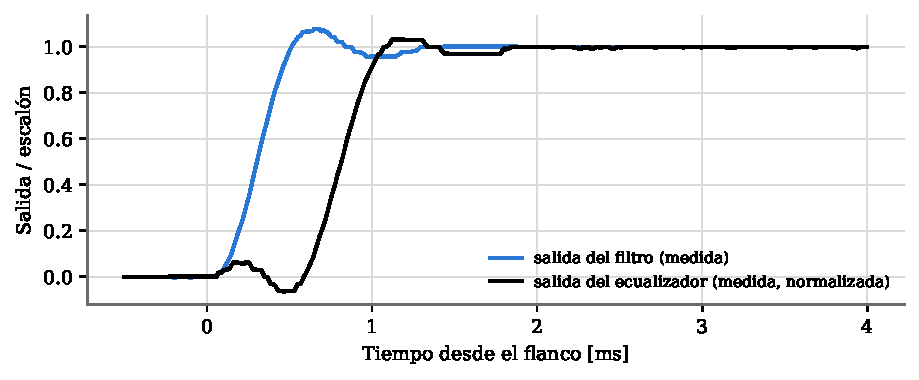
\includegraphics[width=0.9\textwidth]{fig_ec_medicion_escalon}
  \caption{Respuesta medida a una onda cuadrada de \qty{2}{\volt} pico a pico: salida del filtro y salida del ecualizador, cada una normalizada
  por su escalón.}
  \label{fig:ec_medicion_escalon}
\end{figure}
\else
\pendiente{respuesta a la onda cuadrada con el ecualizador final (\texttt{escalon\_cascada.csv}).}
\fi

\section{Conclusiones}
\label{sec:conclusiones}

\paragraph{Elección del filtro.} De los cuatro diseños que cumplen la plantilla, se implementó el pasabajos Chebyshev~I de orden~3. Es una función
todo polos, de orden impar y $Q$ moderado, que se realiza con una red RC con seguidor y un Sallen--Key de ganancia unitaria en un solo TL072, y tiene
casi \qty{18}{\decibel} de margen a \qty{4}{\kilo\hertz}. Su desventaja, el retardo de grupo variable cerca del borde de paso, se trató en el
Nivel~III.

\paragraph{El margen de diseño fue la decisión clave.} La función de la plantilla tiene exactamente \qty{1}{\decibel} de rizado, y con componentes
reales solo cumpliría alrededor del \qty{\vRendSinMargen}{\percent} de los filtros construidos. Sintetizar en cambio una función con
\qty{\vApD}{\decibel} de rizado y borde en \qty{\vFpD}{\hertz} cambia la atenuación a \qty{4}{\kilo\hertz}, que sobraba, por tolerancia en la banda
de paso, que faltaba. El prototipo lo confirma: sus capacitores se apartan hasta un \qty{10}{\percent} del nominal y aun así su atenuación máxima en
la banda de paso es de \qr{2}{\mApMaxMed}{\decibel}. Con los mismos desvíos, el filtro sin margen tendría \qr{2}{\mApSinMargen}{\decibel} y no
cumpliría la plantilla.

\paragraph{El prototipo cumple la plantilla y el modelo lo explica.} La atenuación a \qty{4}{\kilo\hertz} es de \qr{1}{\mAcuatrokMed}{\decibel},
con \qty{11}{\decibel} de margen sobre los \qty{24}{\decibel} exigidos. El modelo ajustado a la ganancia y la fase medidas describe la medición
dentro de la incertidumbre ($\chi^2_\nu = \nr{2}{\mChiCuadRed}$). Los capacitores estimados a partir de ese ajuste, junto con las resistencias
medidas y las sensibilidades de la \cref{sec:sensibilidad}, predicen una variación de la ganancia a \qty{1}{\kilo\hertz} de
\qr{2}{\mDGunokPred}{\decibel}; la medida es de \qr{2}{\mDGunokMed}{\decibel}. Como anticipaba el análisis de sensibilidad, los capacitores, y no
las resistencias ni el AO, determinan cuánto se aparta el filtro real del nominal.

\paragraph{Cadena de validación.} Cada etapa se contrastó con la anterior y todas coincidieron dentro de su incertidumbre: la derivación simbólica
con SymPy, el circuito ideal en LTspice (diferencia menor que \qty{1e-4}{\decibel}), el modelo del TL072 (cuyo único efecto apreciable en la
banda de interés es el GBW finito) y la medición. Las discrepancias que aparecieron tuvieron causas identificables y documentadas: la compresión de
formas de onda de LTspice en la respuesta al escalón, la fuga del Sallen--Key de ganancia unitaria por encima de \qty{40}{\kilo\hertz} y el piso
de medición del osciloscopio en la banda de rechazo lejana.

\paragraph{Nivel~II.} El Monte Carlo de \nNRun{} corridas distintas por escenario en LTspice estima un rendimiento del \qty{\nRendLtDos}{\percent}
con los componentes usados, en acuerdo con Python (\qty{\nRendPyDos}{\percent}) y con la predicción por sensibilidades
(\qty{\nRendLinDos}{\percent}). Con tolerancias de hasta \qty{10}{\percent}, el filtro se comporta de forma prácticamente lineal y la fórmula de
propagación de sensibilidades basta para estimar la dispersión, aunque no la forma de la distribución. Todas las fallas se deben al rizado, por
el desvío de los capacitores: con capacitores de \qty{\pm 5}{\percent} cumple el \qty{100}{\percent} de los circuitos, mientras que mejorar las
resistencias aporta poco.

\paragraph{Nivel~III.} Un pasatodo de 2.º orden con un solo AO, diseñado para el prototipo y no para el filtro nominal, redujo la variación del
retardo de grupo en la banda de paso de \qr{4}{\eMJFil}{\milli\second} a \qr{4}{\eMJCas}{\milli\second}: una mejora de \num{\eMMejora} veces,
con un intervalo del \qty{90}{\percent} de \numrange{\eMMejoraInf}{\eMMejoraSup}. La métrica sin modelo lo confirma: el desvío máximo de la fase
respecto de la fase lineal bajó de \qr{1}{\eMFilDevMax}{\degree} a \qr{1}{\eMCasDevMax}{\degree}. En la respuesta a la onda cuadrada, la
deformación pasa de concentrarse después del flanco a repartirse a ambos lados, como corresponde a un sistema de fase casi lineal. El precio es un
retardo constante adicional de medio milisegundo y una ganancia $k = \num{\eMApK}$; el error de pasatodo remanente es un valle de
\qr{1}{\eMApValle}{\decibel} en $f_0$, con el que la cascada sigue dentro de la plantilla en la banda de paso. La lección principal del nivel es práctica: el óptimo exige $f_0$ y $Q$ con errores de décimas de por ciento, y los
capacitores solo se conocían al \qty{4}{\percent}. El ecualizador alcanzó la mejora porque se sintonizó midiendo: el preset fija la magnitud sin
mover $f_0$ ni $Q$, y la resistencia menor de cada par corrige $f_0$ y $Q$ a partir de los capacitores efectivos deducidos de la medición. La
simulación con los capacitores leídos con el multímetro da una mejora mucho menor, lo que muestra que esa sintonía no se puede reemplazar con
cálculo.

\paragraph{Limitaciones y trabajo futuro.}
\begin{itemize}
  \item \textbf{Capacitores.} Sin medidor LCR, sus valores reales se estimaron en forma indirecta. Un medidor LCR permitiría verificar esas
        estimaciones y calcular el ecualizador sin iteraciones. Para una producción, capacitores de \qty{\pm 5}{\percent} eliminarían prácticamente las
        fallas sin cambiar la topología.
  \item \textbf{Banda de rechazo lejana.} Por encima de unos \qty{4.5}{\kilo\hertz} la medición queda limitada por el piso del instrumento. Medirla
        requiere más amplitud de entrada, promediado o un analizador con más rango dinámico.
  \item \textbf{Gran señal.} El ensayo de recorte no pudo hacerse con la amplitud máxima del generador; puede completarse bajando la alimentación.
  \item \textbf{Ganancia del ecualizador.} La cascada tiene \qr{1}{\eLTEcGananciaDb}{\decibel} de ganancia. Si hiciera falta ganancia unitaria, se
        puede agregar una etapa no inversora o redistribuir la ganancia en el filtro.
  \item \textbf{Respuesta a la onda cuadrada.} La captura final no se tomó en modo de alta resolución, lo que limita la incertidumbre del
        sobrepico a uno o dos puntos porcentuales.
\end{itemize}

En síntesis, el filtro construido cumple la plantilla con margen, y cada resultado medido se explica con el diseño, la sensibilidad y la
simulación. Los dos niveles optativos agregan la cuantificación estadística del rendimiento y una mejora medida de más de diez veces en la
linealidad de fase. Todo el trabajo es reproducible desde los notebooks, los netlists y los datos del repositorio.


\clearpage
\bibliographystyle{babunsrt}
\bibliography{referencias}

\end{document}
